% !TeX program = lualatex
% UCF ETD accessible PDF setup.
% This file must be loaded before \documentclass.
% Students should not need to edit this file.
\ifx\directlua\undefined
\DocumentMetadata{
  lang=en-US,
  pdfstandard=ua-2,
  pdfstandard=a-4f,
  tagging=on
}
\else
\DocumentMetadata{
  lang=en-US,
  pdfstandard=ua-2,
  tagging=on,
  tagging-setup={
    math/setup=mathml-SE
  }
}
\fi
\documentclass{UCF_ETD}
\usepackage{amsmath,booktabs,array,longtable,tabularx,xurl,enumitem}
\setlist{itemsep=3pt,topsep=5pt}
% Preserve the UCF chapter appearance while exposing its custom headings to
% the same tagged section hierarchy used by ordinary LaTeX section commands.
\makeatletter
% luatex.def adds a second /Group dictionary to imported Cairo PDFs, which
% already carry their own transparency group. Preserve the source group.
\ifdefined\directlua
  \def\Gread@pdf#1{%
    \let\Gin@decode\@empty
    \Gin@interpolatefalse
    \Gread@transgroupfalse
    \Gread@pdftex{#1}%
  }
\fi
\newcommand{\thesis@chaptertagbegin}[1]{%
  \par
  \UseTaggingSocket{sec/end}{0}%
  \UseTaggingSocket{sec/begin}{{0}{}}%
  \begingroup
  \UseTaggingSocket{sec/title/begin}{{0}{#1}}%
}
\newcommand{\thesis@chaptertagend}{%
  \par\UseTaggingSocket{sec/title/end}\endgroup
}
\let\thesis@makechapterhead\@makechapterhead
\renewcommand{\@makechapterhead}[1]{%
  \thesis@chaptertagbegin{#1}%
  \thesis@makechapterhead{#1}%
  \thesis@chaptertagend
}
\let\thesis@makeschapterhead\@makeschapterhead
\renewcommand{\@makeschapterhead}[1]{%
  \thesis@chaptertagbegin{#1}%
  \thesis@makeschapterhead{#1}%
  \thesis@chaptertagend
}
% Keep longtable captions outside the grid so they are Caption structures,
% not merged TH cells. The surrounding group limits these settings to one table.
\newcommand{\thesislongtablecaption}[2][]{%
  \par
  \def\@captype{table}%
  \if\relax\detokenize{#1}\relax
    \caption{#2}%
  \else
    \caption[#1]{#2}%
  \fi
  \stepcounter{LT@tables}% Unique destination for the unnumbered longtable grid.
  \renewcommand{\LTcaptype}{}% Caption already advanced the table counter.
  \setlength{\LTpre}{0pt}% Caption supplies the preceding spacing.
  \nopagebreak
}
\makeatother
\graphicspath{{figures/}}
\emergencystretch=2em
\setcounter{tocdepth}{2}
\clubpenalty=10000
\widowpenalty=10000
\displaywidowpenalty=10000
\raggedbottom
\newcommand{\qid}[1]{\par\smallskip\textbf{\texttt{#1}}\par}
\newcommand{\draftnote}[1]{\par\noindent\textbf{Draft status.} #1\par}
\title{FOLLOW MY VOICE: SELF-SIMILAR AND NEUTRAL VOICES FOR GAZE-CONTINGENT OBJECT SEARCH IN MIXED REALITY}
\author{PEDRO POVEDA QUEVEDO}
% Previous degree and major professor omitted pending author confirmation.
\thesisname{thesis}
\degreename{Master of Science}
\departmentsname{Computer Science}
\collegename{Engineering and Computer Science}
\termname{Fall}
\termyear{2026}
\begin{document}
\frontmatter
\maketitle
\copyrightpage{~Pedro Poveda Quevedo}
\begin{aidisclosure}
This first-pass manuscript was prepared with assistance from OpenAI Codex for source organization, drafting, implementation-to-protocol reconciliation, and LaTeX production. Claude performed separate language and methods reviews; their findings and the changes made in response are recorded with the source project. The author must review the manuscript, verify its citations and claims, and approve the final disclosure before submission. This working disclosure does not assert that author validation or committee approval has already occurred.
\end{aidisclosure}
\begin{abstract}
Directing users' attention to objects of interest has long been a concern in virtual reality, particularly when relevant objects lie outside the user's current field of view~\cite{grogorick2017subtle,lange2020hivefive}. Research in augmented reality has shown that auditory guidance, including verbal hints, can support object search~\cite{zhang2023seehear}. Spoken assistance can connect spatial instructions with objects in the surrounding environment, guiding users toward a region and then the intended object. Beyond the content of spoken instructions, voice identity may influence the experience of receiving assistance. Research on virtual collaboration has found that self-similar voices can increase likability and believability while also eliciting greater eeriness~\cite{guo2024doppelganger}. These findings motivate examining how self-similarity affects users when the voice serves as a spatial guide. This thesis compares gaze-contingent guidance spoken in a synthetic voice resembling the participant's own with guidance spoken in a neutral voice selected by the participant from a supplied catalog.

Follow My Voice will investigate this comparison in a within-participant mixed-reality user study. Participants will complete one practice trial in their first assigned voice and two counterbalanced blocks of 40 measured trials. Seated participants will search colored geometric objects on eight surrounding vertical planes, including locations initially outside their field of view. The participant will not be told the target's identity; instead, gaze-contingent spoken directions will guide orientation toward its region and progressively refine the search. Participants will select the inferred target using the right-controller ray and trigger. Both conditions will use the same guidance policy and phrase library to focus the comparison on voice.

The study will compare active search-completion time, perceived workload, motivation, and agent experience. Voice-similarity ratings and debriefing will examine whether participants recognize the resemblance and how they perceive receiving guidance in their own synthetic voice. Condition-specific questionnaires will be administered after both blocks. This thesis presents the apparatus and study plan; participant results are not yet available.
\end{abstract}
\chapter*{PREFACE}
This is an advisor-review draft revised October 23, 2026. It expands the project's current Overleaf manuscript and bibliography into a thesis using the supplied UCF ETD LuaLaTeX template. It is not a completed empirical report. Present-tense system descriptions refer to the documented implementation snapshot; future-tense methods describe the proposed study. Engineering checks, planned measurements, and participant outcomes are kept separate.

The source snapshot is Overleaf revision \texttt{f9f49e4}. The runtime alignment audit dated October 20 is the accompanying implementation record. Appendix~\ref{app:decision-contract} separately documents an October 23 inspection of three working implementation files, with their hashes and uncommitted status retained. That inspection does not update the deployment claims of the October 20 audit. Later software changes require a new reconciliation before submission. Exact pre-cue geometry, balanced vertical allocation, final sample size, and pilot acceptance rules remain explicit readiness requirements. Qualtrics synchronization remains on hold. The author name, degree details, graduation term, previous degree, advisor, acknowledgments, and final AI disclosure require author confirmation; unverified prior degrees and advisor names have not been inserted.

The structural reference is Hoang Bao Truong's 2026 UCF thesis, \emph{Using Inferences from Natural Language Narratives to Improve Video Question Answering}. Its chapter hierarchy, front matter, detailed methods, diagnostic discussion, and appendices inform presentation only. Its prose, experiments, and findings are not evidence for this study.
\tableofcontents
\listoffigures
\listoftables
\mainmatter
\chapter{INTRODUCTION}
\label{ch:introduction}
\section{Motivation and Background}
\subsection{Why Object Search Matters in AR and VR}
Finding the relevant object is often a prerequisite for doing something useful with an augmented or virtual environment. Before following an instruction, inspecting a component, or interacting with task content, a user must connect the system's intended referent with something they can see. Binetti et al. motivate AR visual-search assistance through maintenance, repair, instruction, and training, where a person must locate a real or virtual target in the surrounding scene~\cite{binetti2021outofview}. These application examples explain why search is worth supporting: assistance can help bridge the gap between knowing which item a task concerns and locating that item among competing objects.

Object search also provides a concrete task through which assistance can be studied. Zhang et al. operationalize it as finding a specified book among other books using a head-mounted AR interface~\cite{zhang2023seehear}. Their task brings together an intended target, distractors, and a search environment without requiring an entire industrial workflow. This makes it a useful precedent for investigating guidance, although finding a book is not evidence that the same interface will improve maintenance or training. The practical motivation and the scope of the evaluation must remain distinct.

In VR, the corresponding challenge is often directing attention without taking away the user's freedom to explore. HiveFive motivates guidance through the possibility of missing relevant content while looking elsewhere, including in cinematic VR, games, and collaboration~\cite{lange2020hivefive}. This is broader than object retrieval, but it shares the problem of bringing a system-relevant location into the user's attention. Kwok et al. similarly motivate gaze guidance through large search spaces and the example of locating an object described by an audio guide~\cite{kwok2022twostep}. These works justify studying the connection between a cue and its intended referent, rather than assuming that presenting information guarantees that the user will find it.

AR and VR therefore offer related but different reasons to study guided search. AR can connect instructions to the surrounding physical workspace; VR can distribute relevant content throughout a simulated environment. In either case, a cue must help the user orient and identify what matters. The present project uses passthrough mixed reality with surrounding virtual objects as a controlled setting for this interaction. Its intended contribution concerns how people receive assistance, with potential relevance to these wider applications rather than a claim of demonstrated transfer to them.

\subsection{Why the Guiding Voice Matters}
Once assistance is spoken, its usefulness depends on more than the direction encoded in the words. ``Look to your right'' describes an action, but it is also delivered by a voice the listener may welcome, recognize, or find uncomfortable. Research on gaze-contingent auditory feedback and staged guidance establishes precedents for adapting assistance to the search process~\cite{losing2014guiding,kwok2022twostep}. The question pursued here concerns the voice carrying that assistance: would directions feel or function differently if they sounded like the person receiving them?

Self-similar voice is a specific form of personalization. It uses recorded speech to synthesize a voice resembling the participant, whereas catalog personalization lets that participant choose an existing voice. Prior studies connect voice self-similarity with selected engagement and identification outcomes in a game, and with both favorable impressions and eeriness in virtual collaboration~\cite{kao2021selfsimilar,guo2024doppelganger}. These findings make self-similar assistance worth investigating without implying that it is necessarily preferable. A familiar-sounding voice could be welcome in one role and distracting in another; this study asks about the role of a spatial guide.

For designers, the useful question is consequently whether self-similar synthesis offers value beyond a voice the user already likes. Follow My Voice compares a self-similar synthetic voice with a participant-preferred catalog voice, not an intentionally poor or impersonal baseline. If participants find their clone more useful or comfortable, that would support considering resemblance as a design option in this task. If the preferred voice is easier to follow, or if resemblance introduces discomfort, that would be equally relevant to voice selection. No such outcome is assumed in advance.

Usefulness will be evaluated through both behavior and experience. Recognizing the clone is a manipulation check, not a performance benefit; liking it without searching faster is still an experience result. Likewise, completing efficiently while finding the voice eerie would distinguish task effectiveness from acceptability. The thesis therefore examines completion time, workload, motivation, and agent experience separately, rather than treating a faster or more familiar voice as universally better.

\subsection{A Controlled Setting for Self-Similar Assistance}
Follow My Voice studies this comparison in a surrounding object-search task. A seated participant wears a mixed-reality headset and views colored geometric objects distributed across eight vertical planes. The application knows which object is the target, while the participant is not given its color or shape at the start. Spoken directions first guide orientation toward the relevant wall and then refine the search within it. The participant aims a right-controller ray and presses the trigger to select the inferred target; gaze itself does not select an object.

This initially unnamed target gives the voice an ongoing instructional role. Instead of supplementing a target description that the participant can follow independently, the guidance progressively establishes which object is intended. The controlled shapes and surrounding layout make starting geometry and trial events easier to specify across the two voice conditions. They also limit the claim: this is an experiment about receiving personalized spatial assistance, not a simulation of every demand in a repair, training, or everyday retrieval task.

The central comparison holds the assistance mechanism shared while changing the assigned voice. Gaze contingency and constrained agent decisions provide the means for delivering relevant instructions; they are not additional participant treatments. This organization lets the thesis ask whether hearing guidance in one's own synthetic voice changes the efficiency or experience of being guided, while retaining the practical object-search problem that makes those instructions consequential.

\section{Problem Statement}
The central research problem is whether a self-similar synthetic voice changes task performance or the experience of assistance relative to a participant-preferred catalog voice. Answering it requires a comparison in which guidance policy, target-selection mechanics, and intended difficulty distribution remain shared. Reliable adaptive speech is therefore an experimental requirement: its directions must remain appropriate while the participant's gaze and controller move. A direction that was correct when requested can become obsolete before playback. A controller may already point at the target while an older downward correction is still waiting to speak. These failures can influence both search time and perceived responsiveness, thereby contaminating a voice comparison.

Gaze measurements also require careful interpretation. A ray intersecting an object is an observation made by the interaction system; it does not establish that the participant fixated, recognized, or understood the object. Likewise, a nearby-gaze region is a deliberate interface tolerance that may improve usability but cannot substitute for measuring spatial accuracy. Nor does a headset's nominal output rate demonstrate that the application receives distinct gaze observations at that rate~\cite{dunn2024reporting,niehorster2026dataquality}.

The thesis addresses these problems by separating observed evidence, guidance state, model decisions, and delivered speech, and it carries the same distinctions into the analysis. An instruction selected by a model is not counted as spoken until playback starts. A qualified gaze acknowledgment is distinct from a controller acknowledgment, and a controller acknowledgment does not constitute a successful trial until the trigger selection is correct. This separation is necessary both to implement responsive guidance and to explain what the participant actually experienced.

\section{Research Objectives and Questions}
The primary objective is to evaluate self-similar voice as a form of task assistance, using a participant-preferred catalog voice as the comparison within a shared gaze-contingent system. The primary research question is: will active search-completion time differ between self-similar and preferred catalog voices after accounting for absolute starting angle and repeated observations within participants? The contrast is two-sided because the current design does not justify assuming a performance advantage for self-similarity.

Secondary questions concern perceived workload and activity experience. Will the two voices differ on the six workload dimensions and their complete unweighted mean? Will they differ on interest/enjoyment, effort/importance, pressure/tension, or value/usefulness? Because these outcomes concern different constructs, the analysis will preserve those distinctions rather than pool them into a broad satisfaction score.

Exploratory questions concern agent perception, reliance, and the relationship between task difficulty and voice experience. Participants may describe a voice as more responsive or humanlike, may rely on guidance more often, or may experience a cloned voice as familiar or eerie. Such reports will be treated as judgments about an interaction, not as evidence that the system possesses intelligence, emotions, awareness, or an inner voice.

A supporting validation requirement is to make the assistance process inspectable so that technical faults do not masquerade as effects of self-similar voice. Can recorded state and speech history explain why a cue was eligible, why it played or was suppressed, and how long it waited? Can evaluation distinguish a genuinely unhelpful instruction from an acceptable alternative wording? These questions concern system validity and readiness; they support the empirical study but do not replace it.


\subsection{Research-Question Traceability}
The questions are assigned stable identifiers so that the completed results and conclusion can answer the same questions introduced here. RQ1 is the primary empirical contrast; RQ2 concerns secondary experience measures; RQ3 is exploratory. EQ1 identifies an engineering question rather than a fourth participant research question. Table~\ref{tab:rq-map} connects each question to its evidence and analysis. The identifiers organize the existing plan and do not add a new experimental factor or a directional hypothesis.

\begin{table}[htbp]\centering
\caption[Research questions and evidence requirements]{Research-question traceability for the proposed study. No empirical answer is available in this first pass.}
\label{tab:rq-map}
\small\begin{tabularx}{\linewidth}{@{}p{0.12\linewidth}p{0.39\linewidth}X@{}}\toprule
Question & Intended contrast & Evidence and reporting destination \\\midrule
RQ1 & Does self-similar voice change active completion time relative to a preferred catalog voice? & Trial timing and starting geometry; analysis in Chapter~\ref{ch:analysis}, results in Chapter~\ref{ch:evaluation}. \\
RQ2 & Do self-similar and preferred catalog voices differ in workload or motivation? & Paired block-referenced workload and separate IMI subscales; final retrospective administration. \\
RQ3 & How do voices differ in agent perception, voice experience, reliance, and search behavior? & Custom ratings, agent constructs, debrief, and valid search measures; exploratory voice-by-angle comparison. \\
EQ1 & Can the recorded sequence explain eligibility, delivery, and unhelpful guidance? & State, request, and actual playback records; supporting evaluation in Appendix~\ref{app:guidance-support}. \\\bottomrule
\end{tabularx}
\end{table}

The voice-similarity manipulation check will be reported before the outcome contrasts to aid interpretation across questions. It is not an individual exclusion gate. RQ3 includes appealing, eerie, and familiar voice experiences and the exploratory variation of the voice contrast with starting angle.

\section{Scope of the Comparison}
The independent variable is voice condition: participant-preferred catalog voice versus self-similar synthetic voice. Both conditions use gaze contingency, the same semantic phrase library, the same local geometry rules, and the same controller-selection mechanics. Consequently, the study will not isolate the benefit of gaze contingency, short-term memory, the cloud decision agent, or synthetic speech in general. Those are shared system properties.

The task is deliberately narrower than unrestricted navigation. Participants remain seated and rotate their head and chair to search surrounding planes. Guidance such as ``turn left'' concerns orientation within this setup; it does not ask them to walk toward a target. Objects are virtual, the physical room is visible through passthrough, and the target is initially unnamed. Conclusions will therefore be bounded to guided search under these conditions.

The use of one practice trial in the first assigned voice is a current protocol decision. It introduces an exposure asymmetry: whichever voice appears first also appears during practice. Counterbalancing distributes that asymmetry across voices, but does not remove learning or carryover. The analysis must retain period and assigned order, and the report must describe the practice assignment explicitly.

Figure~\ref{fig:comparison-framework} separates the voice manipulation from the shared task. A difference between conditions would require evidence from the planned study; the diagram specifies the comparison rather than predicting its direction.

\begin{figure}[htbp]
\centering
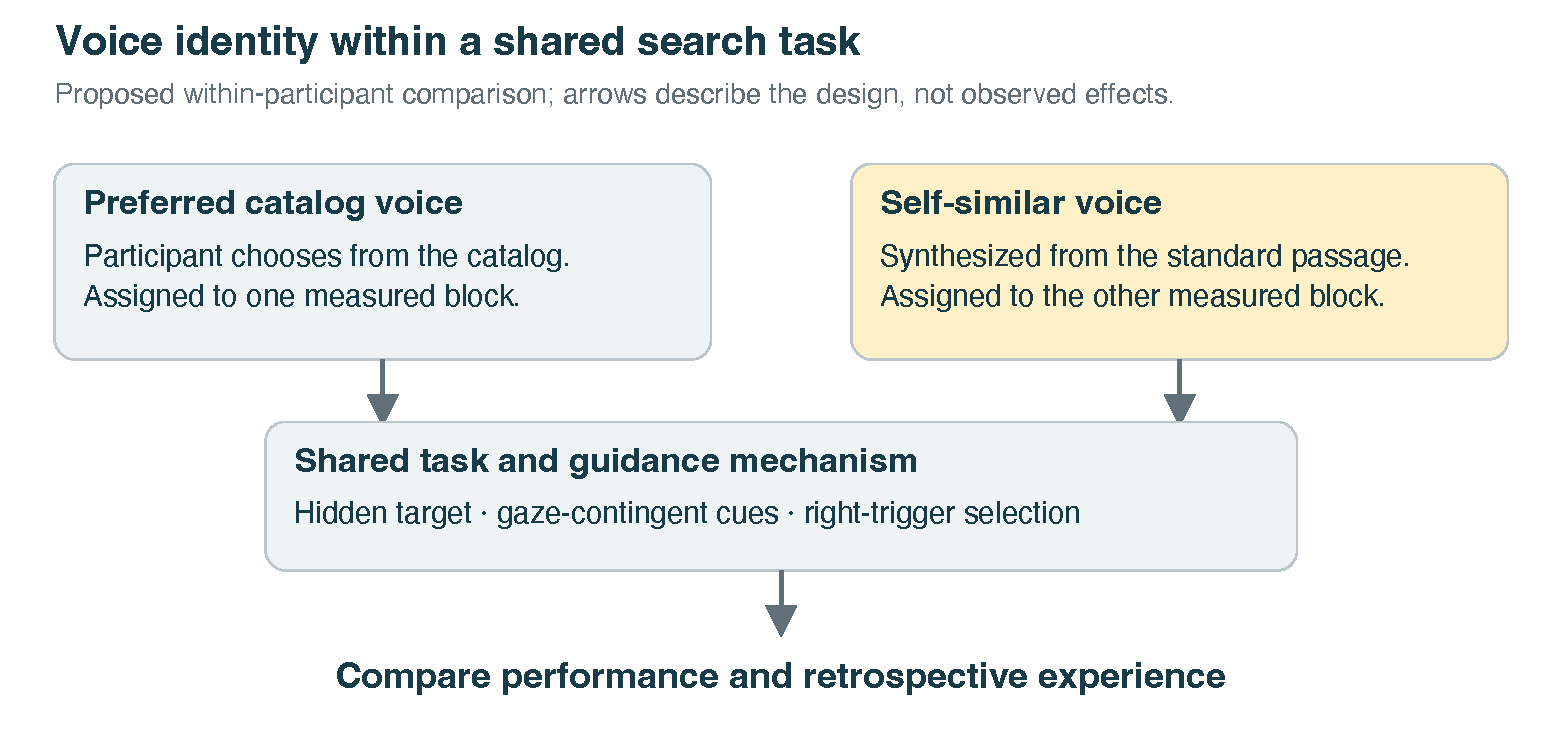
\includegraphics[width=\linewidth,alt={Two voice conditions feed a shared hidden-target search task and a paired outcome comparison.}]{figures/comparison-framework.pdf}
\caption[Voice comparison within the shared search task]{Proposed comparison of preferred and self-similar voices within a shared task and guidance mechanism. The schematic identifies the intended manipulation and outcome families; it does not depict observed effects.}
\label{fig:comparison-framework}
\end{figure}


\section{Contributions of This First Pass}
The thesis develops an empirical comparison of self-similar voice with a preferred alternative in mixed-reality task assistance. Its conceptual contribution is to distinguish resemblance from preference and to examine performance alongside the favorable or uncomfortable experience of hearing one's own synthetic voice. The study will not assume that greater perceived similarity implies faster search, lower workload, or a more welcome agent.

The methodological contribution is a within-participant design that makes this comparison operational: two counterbalanced voice blocks, a shared hidden-target task, explicit trigger selection, comparable starting-difficulty allocations, retrospective voice-referenced questionnaires, and a planned repeated-measures analysis. Manipulation checks and acoustic-quality reporting will help establish what the voice conditions actually delivered before their outcomes are interpreted.

The implemented guidance and recording platform supports that empirical contribution. Local spatial eligibility, constrained agent decisions, prepared speech, and synchronized review make it possible to inspect what each participant heard and whether delivery problems affected the comparison. The platform is the apparatus for studying self-similar voice; a provider benchmark or a new gaze-guidance algorithm is not the thesis's primary claim.

The empirical contribution remains pending. This draft does not report a recruited sample, condition means, significance tests, or participant quotations. A completed thesis will replace the pending results sections with the frozen study's actual voice-condition outcomes and revise its abstract and conclusion accordingly.

\section{Organization of the Thesis}
Chapter~\ref{ch:literature} establishes the voice rationale; Chapters~\ref{ch:system} and~\ref{ch:methodology} describe the apparatus and comparison. Chapters~\ref{ch:measurement}--\ref{ch:analysis} define measurement and analysis, and Chapter~\ref{ch:evaluation} organizes the pending results. The discussion and conclusion address self-similar assistance and its limits. Appendices retain instruments, data definitions, readiness decisions, and implementation details.

\chapter{LITERATURE REVIEW}
\label{ch:literature}
The literature connects two parts of the thesis question: why a voice resembling the listener might change an interaction, and why guided search is a useful setting in which to examine that possibility. Research on voice identity and self-similarity first motivates the comparison with a participant-preferred alternative. Work on search and auditory guidance then explains how spoken assistance can have a sustained role in the task. The review closes with the sensing and contextual requirements needed to make that comparison interpretable.

\section{Voice as a Social and Personalized Interface}
Research on machine-generated speech has considered personality, source attribution, and social presence~\cite{nass1993voices,nass2001personality,lee2005socialpresence}. These perspectives motivate treating voice as more than a neutral transport for words. They do not establish that every listener will form the same impression, or that a social impression necessarily improves task performance.

For this project, personalization has two meanings. Catalog personalization allows the participant to choose among existing voices. Self-similar personalization uses recorded speech to create a synthetic voice resembling that participant. Both forms may produce familiarity or liking, but they operate through different routes. Preference is selected directly in the catalog condition, whereas perceived resemblance must be checked in the self-similar condition. The manipulation is therefore not adequately described as personalized versus generic.

The bibliography also includes work on voice-assistant personality customization and similarity~\cite{snyder2023onevoice}. Personality similarity is conceptually different from acoustic self-resemblance. A listener can prefer a speaking style without hearing it as their own voice, and a close acoustic resemblance can be experienced as uncomfortable. The planned manipulation check asks about perceived voice similarity, while the experience battery separately asks about liking, naturalness, familiarity, and uncanniness.

A related AR navigation system by Yang et al. combines Building Information Modeling with retrieval-augmented generation and compares directional arrows alone with an embodied guide accompanied by the same arrows~\cite{yang2025embodiednavigation}. Its comparison concerns the presentation of navigation assistance, not self-similar voice. It provides a useful contrast for the present framing: the question here is how the guiding voice is experienced within a shared assistance mechanism, rather than whether a new reasoning architecture or visible agent improves navigation. The walking task, destination queries, and embodied interface in that system differ from the seated hidden-target task used here.

\section{Self-Similar Voice and Embodied Collaboration}
Self-similar voice provides the empirical motivation for this study, while auditory guidance supplies the setting in which that voice is encountered. Two particularly relevant studies examine resemblance in different roles: an avatar speaking as the player and a virtual collaborator speaking to the participant. The present study extends this question to a guiding voice without a visible agent body.

Kao et al. analyzed 657 participants in an online programming game, comparing self-similar and assigned dissimilar avatar voices while also manipulating pitch~\cite{kao2021selfsimilar}. Self-similar voice was associated with more puzzles completed, longer voluntary play, and higher similarity identification, competence, relatedness, and immersion. Direct differences on the reported intrinsic-motivation subscales were not significant. These findings motivate examining several dimensions of voice experience rather than assuming that resemblance improves enjoyment or every measure of motivation.

The meaning of performance also changes across tasks. Longer voluntary play in Kao et al.'s game can indicate continued engagement; a longer fixed search trial here can indicate difficulty. Follow My Voice will therefore interpret completion time alongside workload, motivation, and reported reliance, without treating speed as a complete account of the value of self-similar voice. This is a transfer of the research question, not a prediction that the direction of every outcome will replicate.

Guo et al. used a 25-participant, within-subject design crossing appearance and voice self-similarity during virtual jigsaw collaboration~\cite{guo2024doppelganger}. Self-similar voices increased likability and believability ratings while also increasing eeriness. Voice did not significantly affect co-presence or perceived intelligence, although appearance affected those measures. These results support keeping favorable and adverse reactions separate and distinguishing voice effects from effects of a visible character. They do not establish a search-speed advantage.

Both studies compared self-similar voices with assigned alternatives; Follow My Voice instead compares the clone with a participant-preferred catalog voice~\cite{kao2021selfsimilar,guo2024doppelganger}. The substantive question is consequently whether resemblance to oneself offers a different experience from a voice one has already chosen. Recognition of the clone, liking of the voice, and willingness to follow its instructions need not coincide. Keeping these constructs separate makes a mixed outcome informative rather than contradictory.

The distinction between embodiment of the participant and embodiment of the agent is important. Participants wear a headset and use a tracked controller, so the interaction involves physical sensing and action. The guiding agent, however, is not represented by a co-present animated character. Measures adapted from an embodied collaborator must therefore be described as adaptations. Their use does not establish that the same factor structure or interpretation holds for a disembodied voice.

Self-voice applications in daily reminders and emotional self-voice interventions extend the range of contexts represented in the bibliography~\cite{kim2024selfvoice,fang2025emotional}. They motivate asking whether participants can imagine uses for their own synthetic voice. They do not establish that navigation guidance will be more effective or that participants will experience it as inner speech. The debrief consequently begins with open questions before introducing probes about eeriness, self-talk, and possible applications.

\section{Naturalness, Familiarity, and Uncanniness}
Voice resemblance is not the only acoustic difference that listeners may notice. Synthesis can change articulation, prosody, loudness, duration, or perceived naturalness. Research on vocal uncanniness provides a reason to keep these qualities visible rather than subsume them under similarity~\cite{diel2024uncanny}. A clone that is recognizable but difficult to understand is not equivalent to a recognizable and intelligible clone.

The experiment will use the same semantic library and provider for both conditions. This is an implementation control rather than proof of equal acoustics, because prepared clips can differ in duration and pronunciation even when their text matches. Pilot checks will therefore inspect intelligibility and comfortable playback levels across catalog and cloned voices, and the actual provider, model, voice, and library identifiers will identify the configuration each participant heard.

Custom experience items and the appealing, eerie, and familiar items selected from Guo et al. will remain separate, since combining them would imply a measurement model not established for this study. A participant may report a voice as both familiar and eerie, and preserving the individual item directions keeps that response interpretable.

\section{Workload, Motivation, and Agent Perception}
The possibility of both welcome and uncomfortable self-resemblance makes outcome selection part of the research argument. Task speed describes efficiency, while workload, motivation, and agent perception address different aspects of receiving help. The following measures retain those distinctions so that the comparison can reveal a tradeoff rather than require one voice to rank higher on every dimension.

Zagermann et al. discuss eye tracking as a means of investigating cognitive load in visual computing~\cite{zagermann2016workload}. That motivates considering gaze-derived measures, but does not license interpreting an unvalidated ray-hit count as workload. The current confirmatory plan uses subjective workload dimensions and task performance. Pupil, fixation, and saccade analyses remain contingent on separate acquisition and event-validation work.

NASA-TLX supplies six workload dimensions~\cite{hart1988nasatlx}; the project's 0--10 response range and unweighted complete mean are documented adaptations. The Intrinsic Motivation Inventory distinguishes interest/enjoyment from related subscales such as effort, pressure, and value~\cite{ryan1982control,mcauley1989imi,csdtIMI}, and reporting the subscales separately preserves that distinction. The instrument appendix specifies the current wording and reverse keys so that scoring can be reproduced.

Agent perception measures are drawn through Guo et al., with attribution to their originating measures~\cite{guo2024doppelganger,biocca2001networked,moussawi2019perception}. Co-presence, perceived intelligence, and anthropomorphism concern participant attributions, so a high rating does not establish sentience or decision correctness. Conversely, deterministic validity checks do not establish that a participant found the agent natural. The design therefore needs both kinds of evidence while keeping their meanings separate.


\section{Visual Search and Attention Guidance in Extended Reality}
To study a guiding voice, the task must give its instructions a meaningful role. Object search provides that role by requiring the participant to connect guidance with a location and then an intended object. The search literature helps specify this setting; it does not supply the answer to the voice comparison.

Search in a surrounding display differs from search on a single front-facing screen because relevant objects may lie outside the visible field. Turning changes what can be inspected, while eye movements refine attention within the visible region. Work on eye and head movements across an extended field of view is therefore relevant to the task geometry~\cite{stein2024eyehead}. In the present study, this motivates recording both head motion and gaze rather than treating one as a complete substitute for the other.

Several approaches to directing attention in immersive environments inform this design. Grogorick et al. address subtle gaze guidance, while HiveFive concerns immersion-preserving attention guidance~\cite{grogorick2017subtle,lange2020hivefive}. Ariza and colleagues investigate vibrotactile assistance and proximity-based multimodal feedback for selection~\cite{ariza2017vibrotactile,ariza2018proximity}. These works establish relevant design alternatives without implying that all forms of guidance are equivalent: a cue that changes visual salience, a vibration that indicates proximity, and a spoken spatial instruction impose different perceptual and interpretive demands.

RippleVision provides a recent visual counterpart to gaze-contingent spoken guidance. Kudnick et al. describe brightness ripples restricted to a cone between a point of interest and the current gaze location, with opposite brightness modulation in the two eyes~\cite{kudnick2026ripplevision}. This technique description is supported by the published abstract; detailed study methods and comparative outcomes remain outside the present synthesis pending full-text review. Its relevance here is conceptual: assistance can adapt to where a participant looks without specifying the target through spoken identity. It also raises a design question for voice guidance: how much assistance is useful before it becomes intrusive? That question motivates considering participant experience alongside task performance; it does not establish that visual and spoken cues have equivalent effects. Follow My Voice holds its assistance policy common across voice conditions to investigate self-similar voice, rather than comparing guidance modalities.

Binetti et al. examine visual and auditory cues for locating out-of-view objects in head-mounted augmented reality~\cite{binetti2021outofview}, and Warden et al. focus on target cue type and location in augmented-reality search~\cite{warden2022visual}. Together, these studies show why target visibility and cue availability belong in the method description. Follow My Voice does not open with a color-and-shape description of the target; instead, the sequence of directions gradually narrows the participant's search.

This hidden-target design creates an important boundary. A participant who already knows the target can continue searching without further assistance. Here, the participant must obtain enough spatial information to infer which object is intended. The voice may consequently be heard more often and may be more consequential than in a task where it supplements an already known target. That is a reason to describe the task precisely, not a reason to assume stronger voice effects in advance.

\section{Gaze-Contingent Auditory Guidance}
Auditory guidance is not a single technique. A sound can encode gaze error through loudness, indicate a location through spatial rendering, or communicate an instruction through words. Only the last of these necessarily carries the verbal and vocal identity cues central to this thesis. The following studies inform the shared search design while leaving the self-similar voice comparison open.

Losing et al. tested gaze-contingent sonification in a small desktop study with ten participants: the loudness of a flute tone varied with gaze-to-target distance, reaching silence at the target~\cite{losing2014guiding}. Benefits depended on the search task, with the clearest improvement in the difficult number-search condition. This is evidence for linking auditory feedback to current gaze, rather than evidence for any particular spoken phrase. Our adaptation uses short spatial instructions instead of a continuously varying tone so that participants encounter the assigned voice throughout search. Its frequency and timing remain design choices to validate, not benefits established by the sonification study.

Kwok et al.'s Two-Step Gaze Guidance evaluated 69 participants using a three-monitor display and eye tracking, rather than a VR headset~\cite{kwok2022twostep}. Initial spatial-audio orientation followed by finer guidance shortened search times relative to the other tested conditions; accuracy did not differ significantly across conditions. Their implementation also buffered transitions between guidance stages. The transferable idea is a staged change in the information a cue supplies: first orient toward a region, then refine within it. Follow My Voice adapts that structure to wall entry and within-wall directions; the cited study does not validate this headset, spoken wording, full-surround geometry, or transition thresholds.

Binetti et al. provide a complementary headset-based example using visual arrows and spatialized alarm sounds to locate out-of-view targets~\cite{binetti2021outofview}. Adding sound mitigated response-time costs when visual cues and targets occupied different depth planes, but did not remove the corresponding accuracy cost. The study had no sound-only condition. Its relevance is therefore conditional support for an auditory channel when visual guidance is constrained, not proof that speech is superior to visual cues. It also motivates retaining selection errors separately from completion time in the present voice comparison.

Zhang et al.'s 96-participant AR book-search study more directly concerns verbal instructions~\cite{zhang2023seehear}. Its audio hint specified an approximate shelf once at task onset; it was not repeated gaze-contingent speech. In the sub-study without gaze-playback feedback, hint conditions outperformed the control but did not significantly differ from one another. Combined visual/audio advantages over either modality appeared in the second task of the feedback sub-study. These results support considering task completion and workload together, while making cue timing and feedback exposure explicit. They do not establish that continuous spoken guidance or self-similar delivery will be better.

\paragraph{Design synthesis for the voice comparison.}
The resulting design uses a common coarse-to-fine guidance policy to make the two voice conditions comparable. The agent first helps locate the relevant wall, then narrows the search within it; the participant confirms the inferred target with the right trigger. The target's initially hidden identity gives the voice an ongoing instructional role, unlike a single announcement supplementing a known target. Whether hearing that role in one's own synthetic voice changes performance, comfort, motivation, or reliance remains the empirical question.

Guidance during search, acknowledgment of a qualified gaze or controller contact, and feedback after selection are recorded separately. This separation also distinguishes the researcher's Trial Review tool from Zhang et al.'s participant-facing gaze-playback intervention~\cite{zhang2023seehear}. Reviewing a recording to audit delivery does not expose a participant to a learning intervention. Similarly, a success chime cannot explain an earlier change in direction within the same trial, although it may affect subsequent experience. No participant playback intervention is added to the current protocol.

The current study does not include an unguided or gaze-unaware control; both voice conditions receive the same gaze-contingent policy. Earlier project documents that considered a factorial combination of voice and gaze contingency are historical, and their interpretation cannot be transferred to this two-condition design. Any observed difference will therefore concern the assigned voice experience within the shared assistance system.

\section{Context and Short-Term Memory in XR Agents}
EmBARDiment uses gaze-informed contextual memory to support interaction with an embodied XR agent~\cite{bovo2025embardiment}. That approach motivates making recent interaction evidence available to the assistance policy, although Follow My Voice implements a narrower, bounded interaction history. This history records recent spatial progress, actual speech, and guidance transitions, and its retention limits are implementation choices rather than thresholds taken from the cited system; it does not provide long-term autobiographical memory or an inferred model of the participant's mental state. The guiding voice also has no visible agent body, so the present system does not inherit the embodiment of the cited interface.

Memory-Augmented AR Agents and GenLARP represent additional directions in the bibliography~\cite{choi2025memory,yu2025genlarp}. The former is a conceptual framework and the latter a short system description; neither supplies a validated timing threshold for this application. User-aware virtual agents and proactive AR assistance also offer context for designing state-dependent behavior~\cite{gunawardhana2024useraware,li2025satori}. These works position a design problem, rather than prove that this implementation's memory mechanism improves performance.

Short-term history is operationally useful when the same current geometry can have different meanings. A target to the left may be one the participant has not yet approached, or one they have just passed while turning right. A recently delivered cue can make another identical cue unnecessary. History distinguishes these cases only if it records reliable observations and actual playback. Holding this mechanism constant across voices means the study cannot estimate its independent effect.

Feedback specificity offers a further distinction between adaptive assistance and generic encouragement. Zimmerer et al. examined performance-specific feedback from a virtual exercise coach and found changes in selected agent-perception measures without a corresponding effect on motivation~\cite{zimmerer2025feedback}. For Follow My Voice, this distinction motivates describing whether a cue reports observed progress, corrects direction, acknowledges qualified gaze or pointing, or confirms a successful selection. These functions remain common across voice conditions, so the study will compare voice configurations rather than estimate an independent effect of feedback specificity. Results from embodied exercise coaching do not establish an effect on search time in the present task.

\section{Eye-Tracking Quality and Interpretation}
Eye-tracking quality involves more than a nominal sampling frequency. The reporting guidance of Dunn et al. and the data-quality discussion of Niehorster et al. motivate reporting acquisition, validity, spatial performance, and missingness~\cite{dunn2024reporting,niehorster2026dataquality}. The system must establish how many distinct source observations arrive, how old they are when used, and how error varies across the search space.

Validation work on the Vive Pro Eye and tools such as GazeMetrics are methodological resources~\cite{schuetz2022vive,sipatchin2021usability,adhanom2020gazemetrics}. They cannot substitute for validation on the HTC Vive Focus Vision because device model, fit, calibration, coordinate conversion, and task geometry can differ. The protocol therefore requires independent targets across heights, boundaries, distances, and head orientations, and these validation targets must be separate from targets used to estimate an offset correction.

Drewes et al. compare gaze during locomotion in virtual reality and the real world~\cite{drewes2021locomotion}. This study is seated and uses head and chair rotation rather than free walking, so locomotion findings cannot be imported as direct estimates of its gaze behavior. Head motion will be logged because it participates in search, while claims about eye events remain bounded by the available measurements.

Salvucci and Goldberg discuss identifying fixations and saccades from eye-tracking protocols~\cite{salvucci2000fixations}. An interaction region around an object serves a different purpose. The 100-ms vicinity qualification in this system is an interface acknowledgment rule, not a validated fixation classifier. The thesis will report gaze contacts and qualified vicinity events under their own names.

\section{Comparison of the Closest Research Strands}
Table~\ref{tab:related-work-map} compares the selected work by what it contributes to this design and what it leaves unresolved. It is a focused synthesis of the preceding review, not a systematic-review inventory or a ranking of systems. The literature does not supply one interchangeable baseline: spatial guidance, voice resemblance, context management, and measurement quality answer different questions.

\begin{table}[htbp]\centering
\caption[Related research and boundaries of transfer]{Selected research strands and their role in Follow My Voice. These are methodological connections, not evidence that the present implementation reproduces the cited effects.}
\label{tab:related-work-map}
\small\begin{tabularx}{\linewidth}{@{}p{0.26\linewidth}XX@{}}\toprule
Research strand & Relevance to this project & Boundary of transfer \\\midrule
Self-similar voice~\cite{kao2021selfsimilar,guo2024doppelganger} & Motivates the voice manipulation and both favorable and adverse experience measures. & Educational or embodied collaboration tasks do not establish a search-speed benefit here. \\
Auditory and staged gaze guidance~\cite{losing2014guiding,kwok2022twostep} & Supports investigating gaze-dependent, coarse-to-fine assistance. & Does not validate this headset, phrase policy, or gate durations. \\
AR search and task feedback~\cite{zhang2023seehear} & Separates in-task cues from post-task feedback. & Known-target task and feedback manipulation differ from this hidden-target voice comparison. \\
Context-aware XR agents~\cite{bovo2025embardiment} & Motivates explicit recent context for state-dependent assistance. & Does not establish an independent benefit of this bounded memory. \\
Eye-tracking reporting and validation~\cite{dunn2024reporting,niehorster2026dataquality,adhanom2020gazemetrics} & Informs source timing, validity, spatial validation, and gap reporting. & Reporting guidance and other-device results are not Focus Vision accuracy measurements. \\\bottomrule
\end{tabularx}
\end{table}

The resulting contribution is a particular combination of task and comparison. The agent knows an initially unnamed target, the participant receives adaptive spatial speech, and explicit right-trigger selection remains separate from gaze. The empirical manipulation changes the voice configuration while retaining that assistance mechanism. This combination defines the scope of RQ1--RQ3; it does not imply that voice familiarity, memory, and gaze contingency have been independently manipulated.

\section{Synthesis and Research Gap}
The selected literature motivates a focused question about self-similar voice: how does guidance spoken in a synthetic version of the participant's own voice compare with guidance spoken in a preferred catalog voice? Prior voice studies make both favorable and uncomfortable reactions plausible, while audio-guidance studies inform a shared task through which those reactions and performance can be examined. Gaze contingency, staged refinement, and decision support serve that comparison; they are not additional experimental treatments.

The selected work leaves the present comparison unresolved: what changes when the voice guiding an initially unnamed, surrounding object-search task resembles its listener rather than being a preferred catalog choice? The design combines a consequential use for speech with a comparator that already accommodates preference. Its contribution will be to establish how those two voice configurations differ in this setting, including outcomes that favor neither configuration consistently. The next chapter describes the shared apparatus that makes the comparison possible.


\chapter{SYSTEM DESIGN AND IMPLEMENTATION}
\label{ch:system}
Follow My Voice is a gaze-contingent voice guidance system designed to help a seated user find a target object in a surrounding search scene. The system divides responsibility between a local guidance layer, which owns all spatial reasoning, and a cloud language model agent, Jev, which decides how and when to speak. Figure~\ref{fig:architecture} summarizes the pipeline from sensing to speech output. This division makes spatial eligibility logic deterministic and traceable while allowing the agent to adapt the phrasing and timing of guidance to the user's recent behavior.

\section{Apparatus}
The application is developed in Unity 6 (6000.3.10f1) using the Unity OpenXR Plugin (1.16.1), HTC VIVE OpenXR integration (2.5.1), and Unity XR Interaction Toolkit (3.3.1). It is deployed as a standalone Android ARM64 application on the HTC VIVE Focus Vision head-mounted display, with rendering performed locally on the headset using the Universal Render Pipeline (17.3.0). The headset supplies head-pose and eye-gaze tracking, while the tracked right-hand controller supplies pointing and trigger input. Video passthrough supports the mixed-reality view. Network access supports cloud-based agent decisions and voice preparation; it is not used to stream rendered frames from a host computer.

\section{Search Task}
The search task takes place in mixed reality using video passthrough in a neutral physical room. Participants will sit on a swivel chair and interact using the right controller. Virtual colored geometric objects hang on eight vertical planes anchored along the surrounding walls. Figure~\ref{fig:scene} shows the layout from above. The application holds the target identity, which is withheld from the opening instructions, so participants must rely on voice guidance to locate it. Participants select an object by pointing the controller ray at it and pressing the trigger. Stimulus density and spatial bounds will be frozen for the study release after seated-comfort and ray-selection pilots. For each trial, the system logs object positions, layout seed, wall assignment, and target identity.

\begin{figure}[htbp]\centering
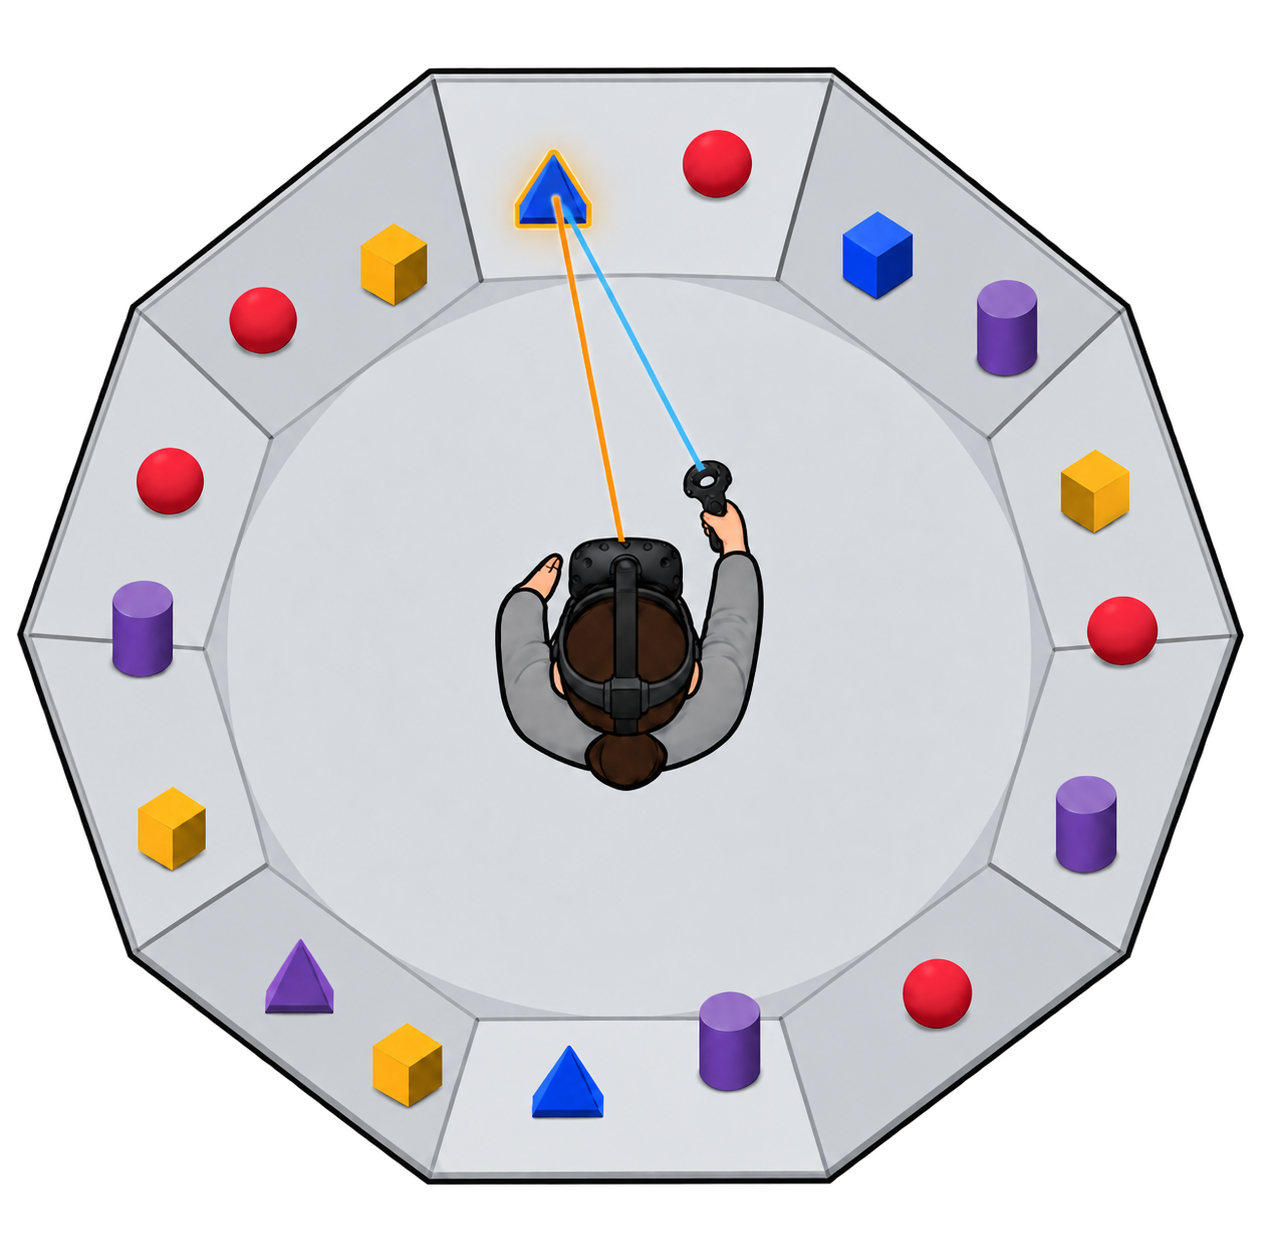
\includegraphics[width=0.70\linewidth,alt={Overhead scene illustration showing a seated headset wearer, surrounding vertical object panels, and gaze and controller rays.}]{figures/image.png}
\caption[Search-scene illustration]{Top-down view of the search scene. The seated participant is surrounded by wall panels holding colored geometric objects. The gaze ray (orange) and controller ray (blue) converge on the highlighted target, the state in which the participant is ready to select with the trigger. The layout is illustrative; the drawn object count is schematic; object positions and target identity vary by trial. The converging rays and highlighted endpoint illustrate interaction, not an advance participant-visible target-identification cue.}
\label{fig:scene}
\end{figure}

\section{Sensing and Guidance State}
The system continuously collects eye-gaze origin, direction, and validity; head pose; right-controller pose; and ray-object intersections. A local state machine combines these observations with the target geometry to track the participant's progress through the search: turning toward the target wall, refining within the wall, acquiring the target with gaze, pointing with the controller, and becoming ready to select. Additional states cover suspended or paused operation. Each state transition is logged with its cause.

Because guidance is only as reliable as the evidence behind it, the state machine issues new gaze-dependent guidance only when gaze data are valid and recent. Gaze ray hits, gaze-vicinity candidates, and controller hits are treated as separate observations. When gaze-vicinity regions overlap, the closest object is chosen as the vicinity candidate. A controller ray hit on the target immediately suppresses contradictory directional cues. The spoken pointing acknowledgment separately requires a one-second controller hold with valid nearby gaze when speech is admitted. Suppression is intended to prevent away-directions during the qualification interval without falsely acknowledging an unqualified hold. Gaze confirmation, controller confirmation, and trigger selection are recorded as distinct events.

\section{Short-Term Interaction Memory}
To give guidance continuity, the system maintains two short-term memories. A spatial history tracks turning progress and supports cues that return the participant to the target. A speech-decision memory records what the system actually said and how the guidance state changed. Each speech entry stores its relative age, context, and whether playback completed or was interrupted; each state entry stores the prior and current states and the reason for the transition. The speech and transition lists each retain at most four entries; snapshots sent to Jev exclude entries older than 15 seconds. This bounded recent context is related to the context-management motivation of EmBARDiment~\cite{bovo2025embardiment}, but the current implementation does not use its object-admission or dropout policy. The separate spatial history retains up to three seconds or 384 target-relative gaze observations and clears on invalid evidence, source changes, or observation gaps longer than 100~ms. These limits are engineering settings, not validated fixation or blink thresholds. Gaze-vicinity confirmation currently requires 100~ms of valid qualifying evidence; invalid evidence resets its entry timer, and reacquisition after a spoken confirmation requires 150~ms of valid gaze away. Those interaction gates do not admit objects to speech memory, and missing gaze is not counted as observed dwell. Both memory types are cleared whenever guidance resets and is copied before each asynchronous request. This memory is deliberately scoped to the current task: it does not build a persistent participant profile or attempt to infer unobserved mental states.

Figure~\ref{fig:bounded-memory} shows which recent evidence accompanies an asynchronous request. Its time limits bound the software context and must not be interpreted as estimates of human short-term memory.

\begin{figure}[htbp]
\centering
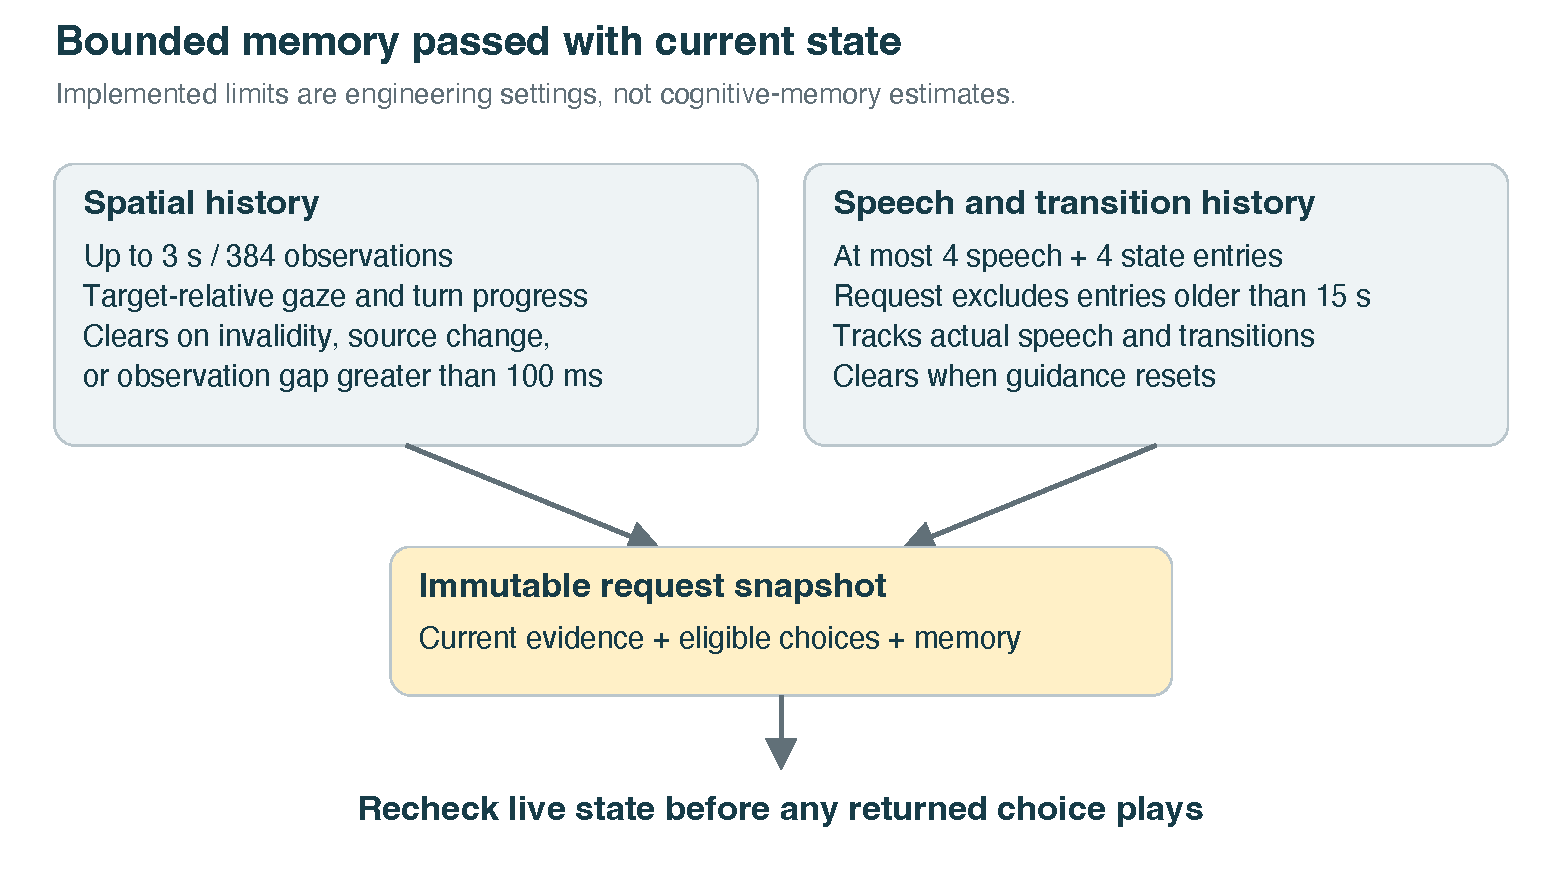
\includegraphics[width=\linewidth,alt={Spatial history and recent speech and state history are copied into a request and checked against current state before playback.}]{figures/bounded-memory.pdf}
\caption[Bounded spatial and speech memory]{Implemented memory limits and snapshot boundary. Spatial history and speech/state history have different retention and reset rules. A copied request preserves its original context, while playback still requires a fresh state check.}
\label{fig:bounded-memory}
\end{figure}


\section{Agent Decisions and Playback Control}
Jev selects from a constrained set of options rather than generating free-form instructions. Local geometry and state rules first filter the phrase library to candidates that are valid in the current situation. Each request to Jev contains a state snapshot, recent memory, playback status, and two to five eligible phrases. Jev then chooses the wording and whether to speak now or wait. Target definition and geometric reasoning remain local. Eligibility filtering and playback revalidation are intended to reduce spatially incorrect or stale guidance, but tracking error, imperfect geometry and software faults can still produce unhelpful instructions; recorded-sequence and headset checks remain necessary.

Because cloud responses arrive asynchronously, the participant's state may change before a decision returns. A local speech scheduler therefore revalidates each decision against the current state, evidence, pacing, and object intersections before playback, and discards decisions that are stale or conflict with the current situation. Qualified gaze and controller acknowledgments and eligible turn-progress milestones can use local handling and are played from prepared phrases without waiting for a new cloud decision, subject to the same checks. Each completed or interrupted utterance updates both the memory and the event log. Model latency, deferral, cancellation, fallback, and playback onset are logged separately to support delay attribution. When a trace lacks the required events, the cause remains unknown rather than inferred from the spoken phrase alone.

\begin{figure}[htbp]\centering
\IfFileExists{figures/voice-guidance-memory-architecture.pdf}{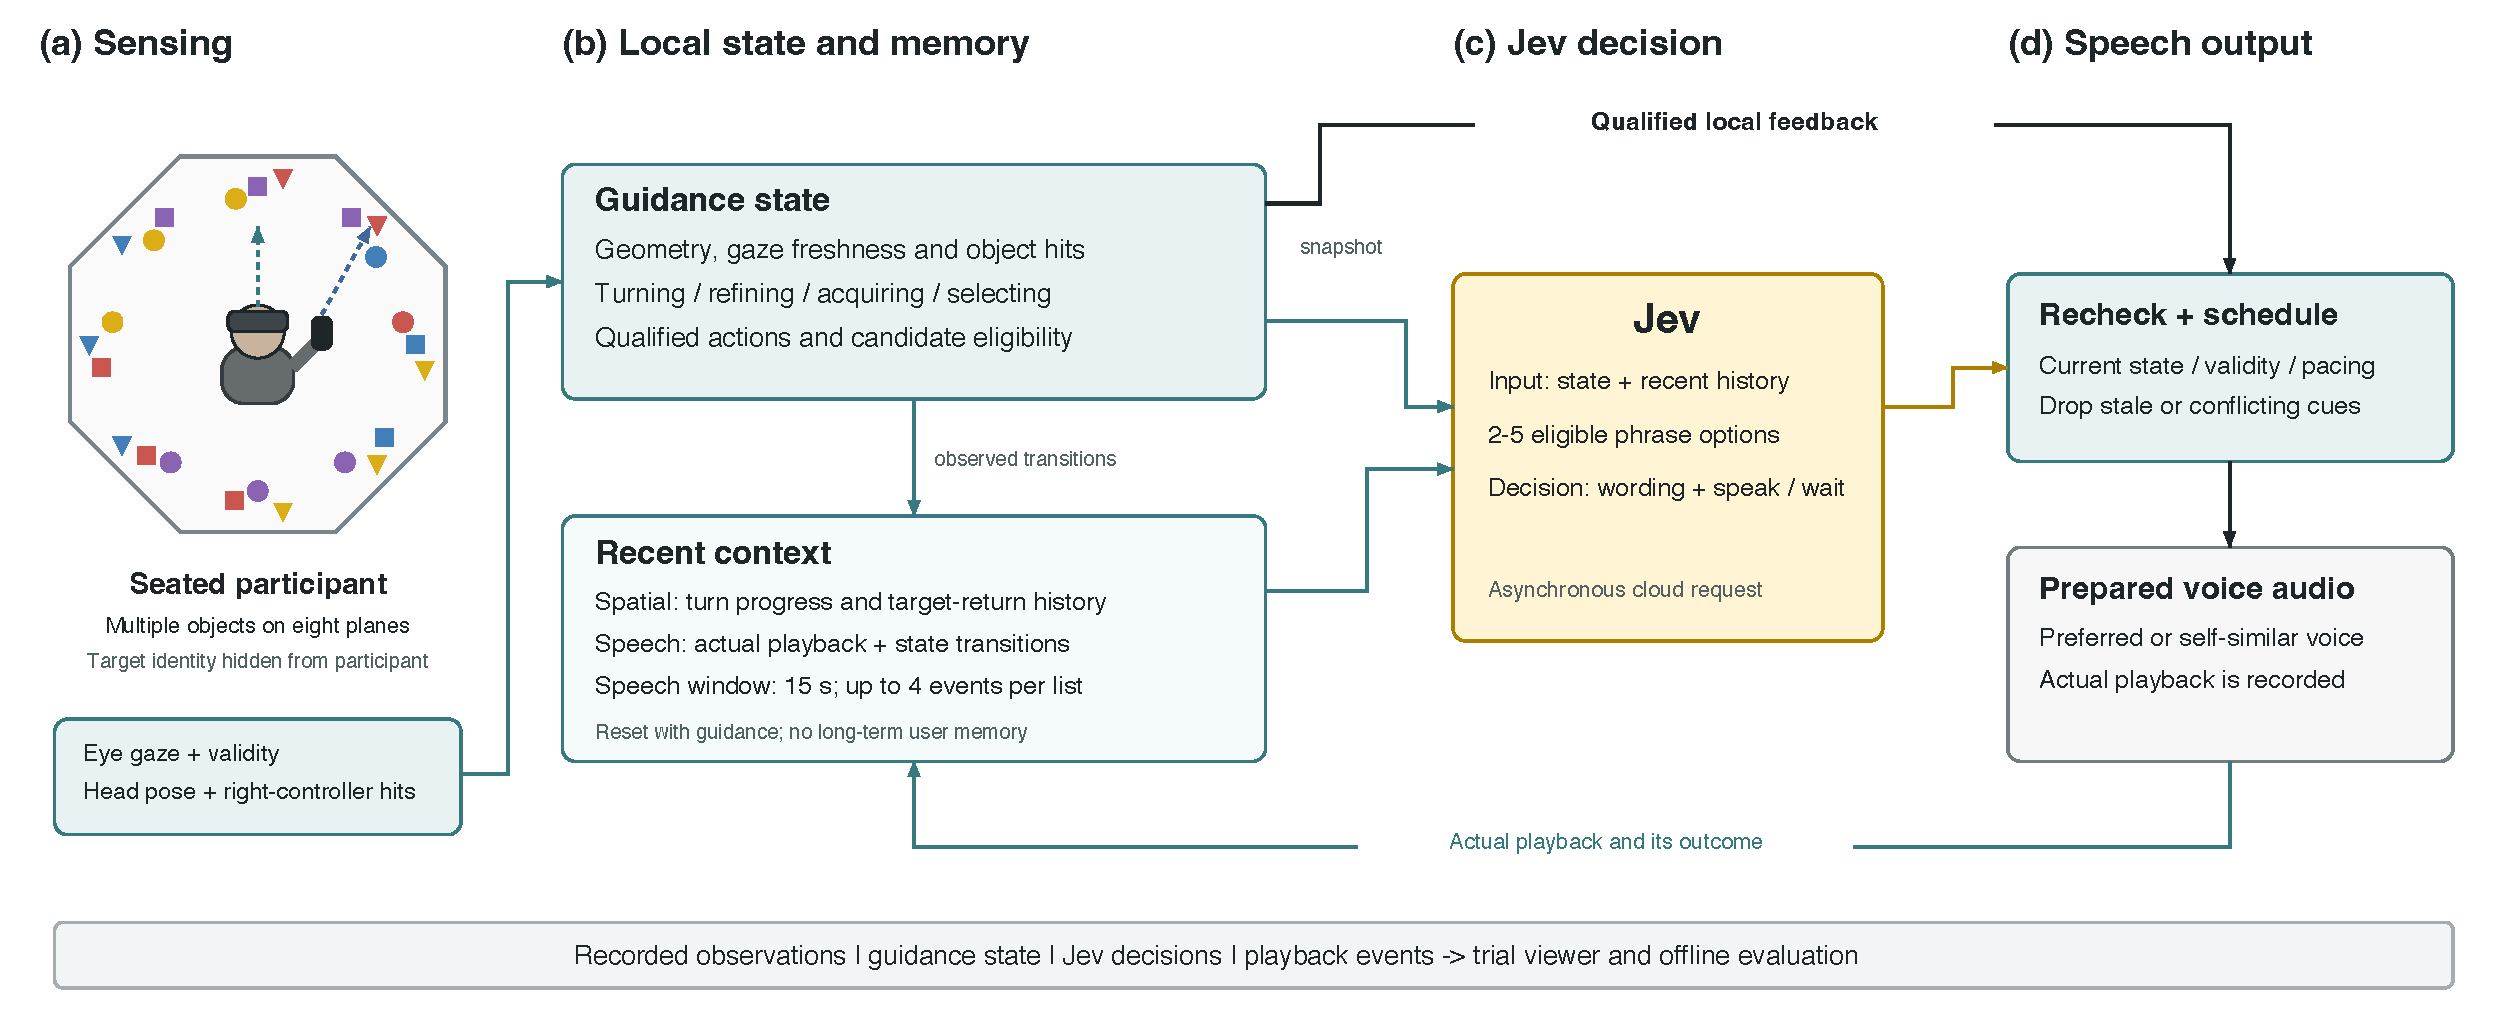
\includegraphics[width=\linewidth,alt={Gaze and controller sensing feed local state and memory, constrained Jev choices, a fresh playback check, and actual speech feedback.}]{figures/voice-guidance-memory-architecture.pdf}}{\fbox{\parbox{0.94\linewidth}{Gaze and controller observations $\rightarrow$ local state and bounded context $\rightarrow$ eligible choices for Jev $\rightarrow$ current-state recheck $\rightarrow$ prepared voice playback. Qualified local feedback also enters the recheck stage.}}}
\caption[Guidance architecture and playback control]{System architecture. (a) Gaze, head, and controller data are sensed. (b) A local state machine and short-term memory determine which guidance actions are valid. (c) Jev chooses wording and timing from eligible options. (d) The scheduler revalidates each cue against the current state before playback. Actual playback feeds back into memory. The scene inset is schematic and does not reflect stimulus count or any participant-visible target cue.}
\label{fig:architecture}
\end{figure}

\section{Voice Preparation and Telemetry}
All voice audio is pre-synthesized with ElevenLabs, which supplies both the catalog voice and the self-similar voice. To support the self-similar condition, each participant records the same standard passage in their usual speaking voice. Both conditions share the semantic phrase library, guidance policy, and playback routing. Voice condition is the intended manipulation; behavior-dependent wording, hint counts and synthesized acoustics need not be identical. The preparation pipeline checks wording and library readiness. Per-voice intelligibility, loudness and acoustic comparability still require pilot verification; automated checks do not establish perceptual equivalence. No pitch or spatial effects are applied to the self-similar voice. We log the provider, model, voice ID, library version, and synthesis settings.

The Trial Review application aligns gaze and controller state, guidance transitions, agent decisions, and playback events with trial geometry on a common timeline. Trial-level aggregates are stored separately from the raw gaze, motion, and event streams. Effective gaze sampling rate must be verified from distinct source timestamps on the tested headset build rather than inferred from the nominal specification or application polling rate. Similarly, the analysis will report ray intersections as gaze hits and do not label them as fixations unless a validated event classifier is applied.

\section{Trial Review Interface}
Figure~\ref{fig:trial-review-synthetic-demo} shows the standalone Trial Review application with its bundled synthetic demonstration. The scene and inspector share a timeline with speech, gaze, events, and decision tracks. The application also supports receiving headset records for live review; transfer and receipt times are separate from source event times, and late arrival must not be interpreted as delayed headset guidance. This capture illustrates the review interface only; it is not a participant recording or a performance result. In particular, the demonstration explicitly marks state history as missing and highlights as reconstructed. That distinction is useful when reviewing legacy records: the viewer should expose unavailable evidence rather than imply it was measured.

\begin{figure}[htbp]
\centering
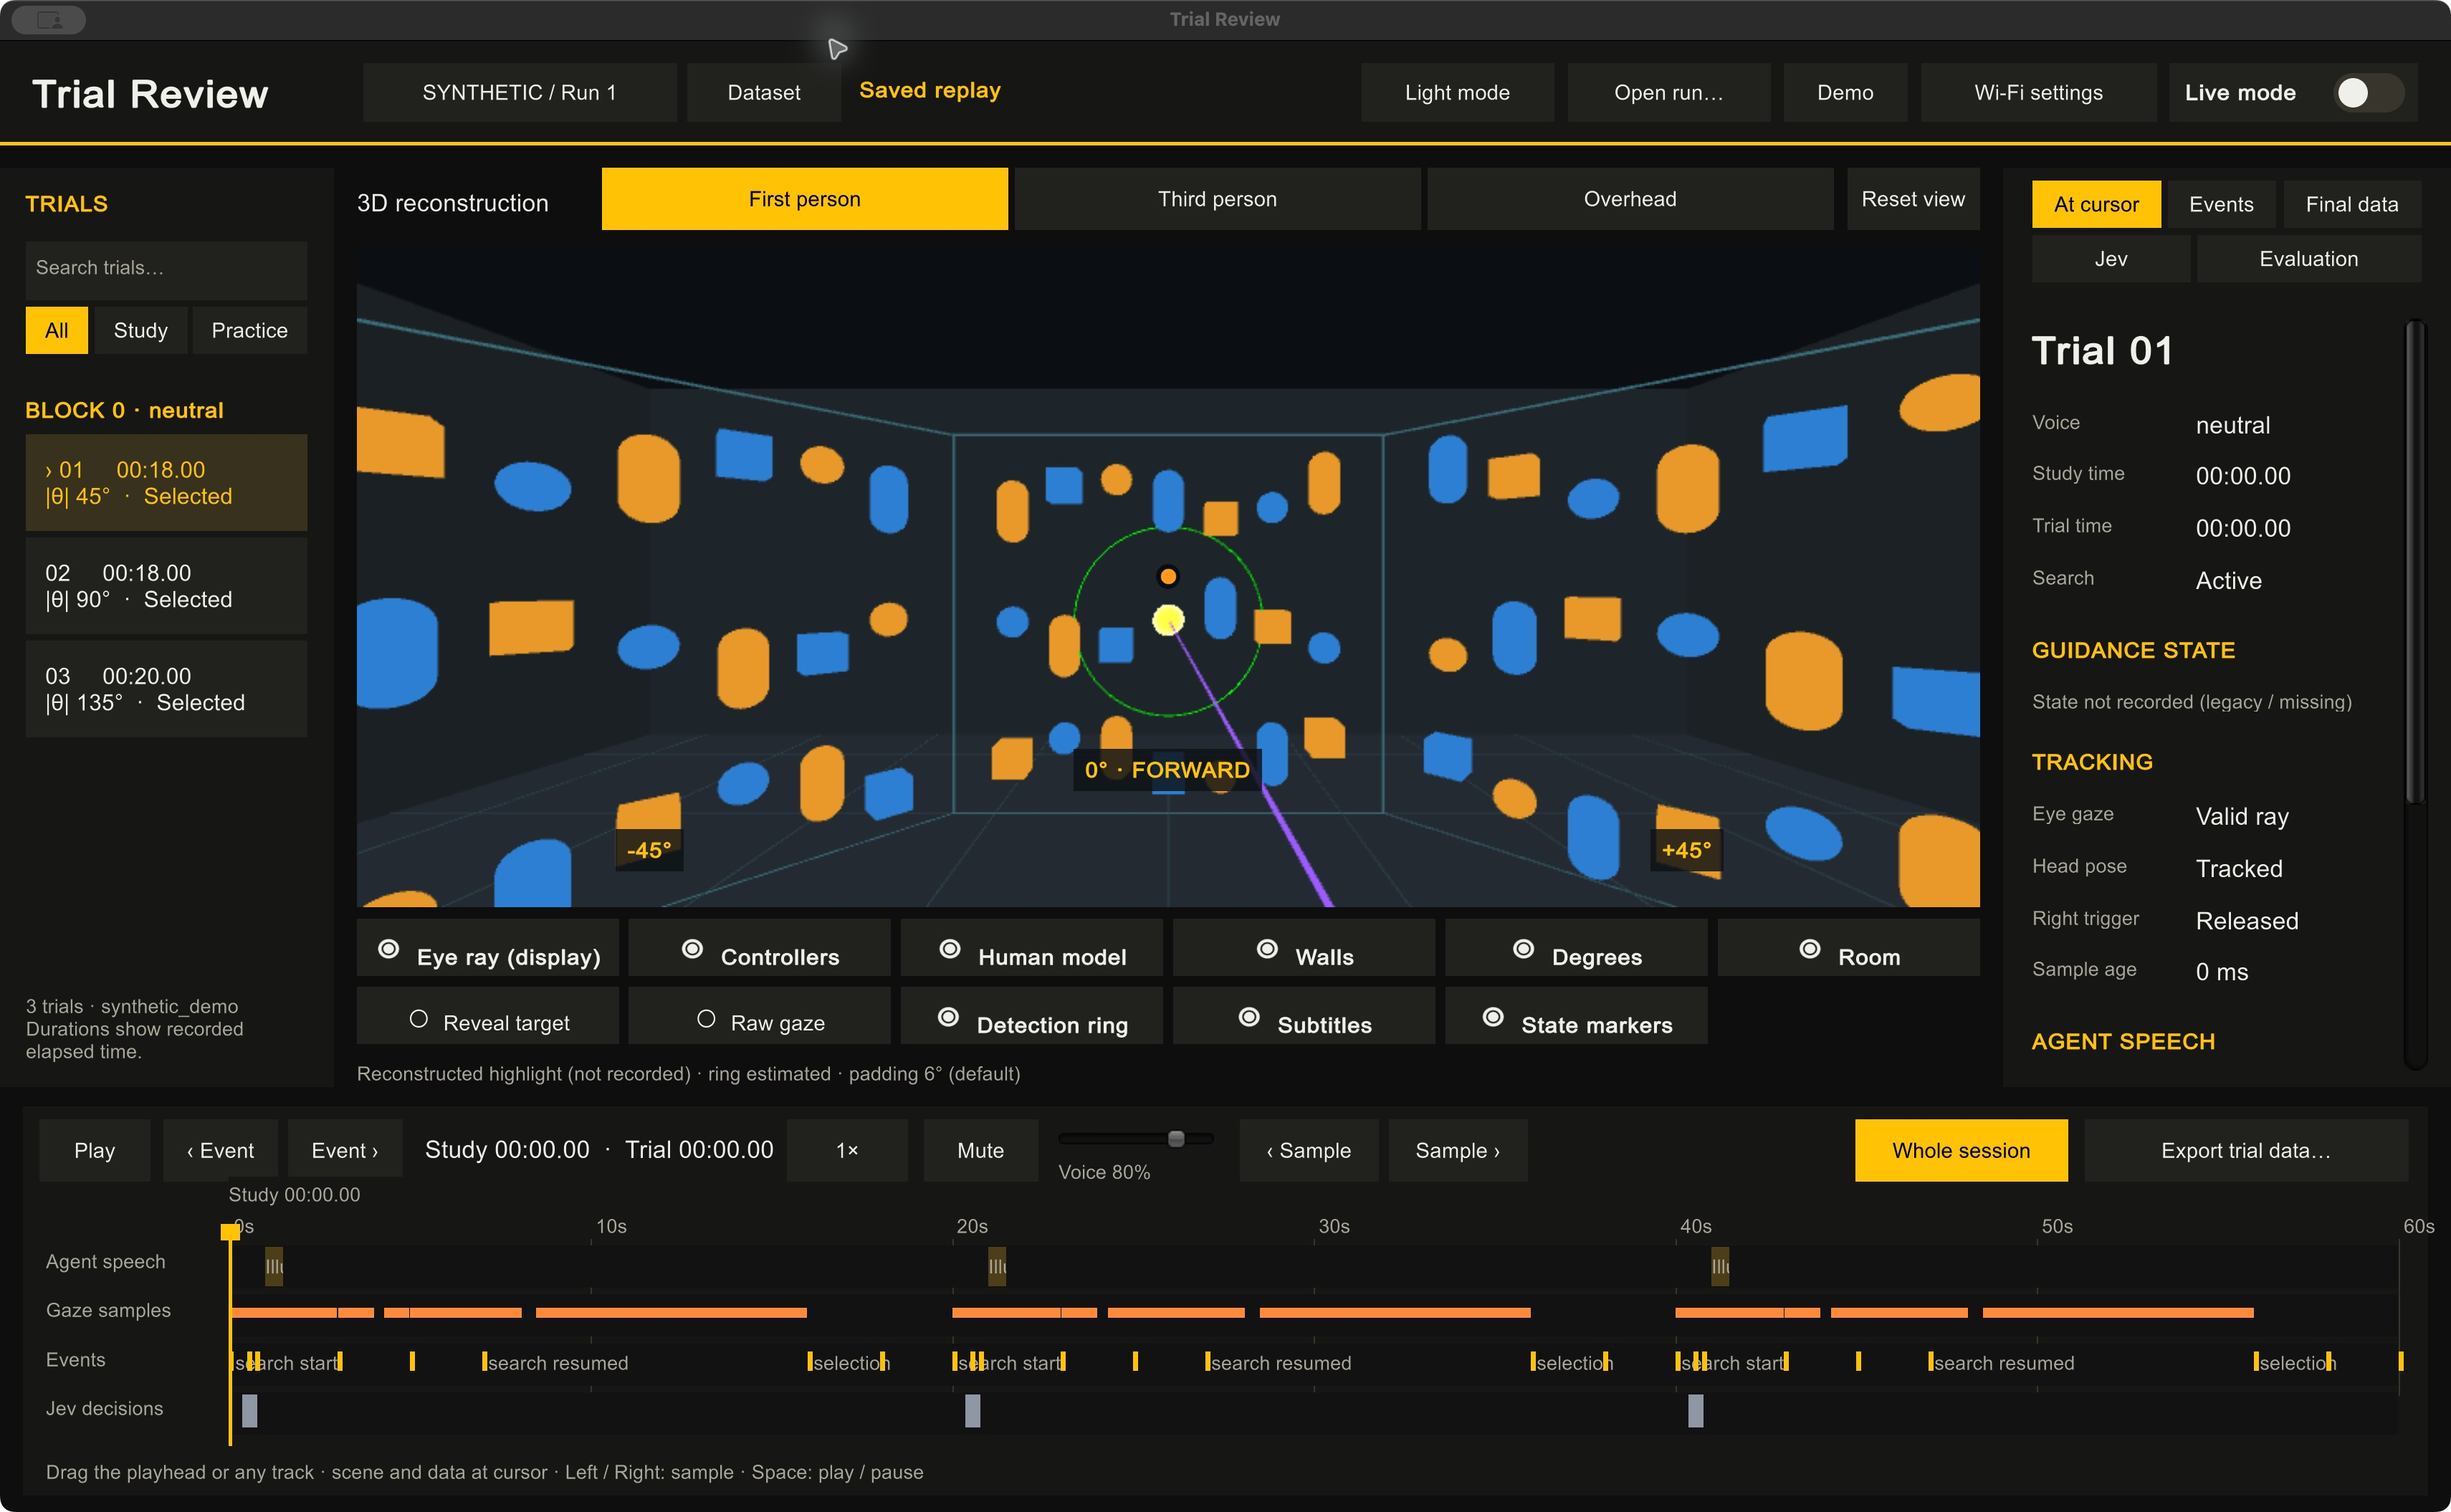
\includegraphics[width=\linewidth,alt={Trial Review application showing its explicitly synthetic three-trial demonstration, reconstructed scene, evidence inspector, and synchronized timeline.}]{figures/trial-review-synthetic-demo.png}
\caption[Trial Review interface with synthetic demonstration]{Actual application screenshot captured for this draft using the bundled SYNTHETIC / Run 1 demonstration. The central reconstruction, right-hand inspector, and timeline provide synchronized review. Missing state, estimated rings, and reconstructed highlights are labeled by the application. This is a visualization example, not headset video or empirical study data.}
\label{fig:trial-review-synthetic-demo}
\end{figure}


\section{Ownership and State Transitions}
The central guidance machine is a plain C\# object, while Unity MonoBehaviours connect it to tracked devices, scene objects, and audio. This separates deterministic state transitions from engine callbacks. The round manager owns readiness, trial onset, completion, pause intervals, and block progression. The guidance machine owns the interpretation of evidence during search. The speech scheduler owns pending requests, cancellation, and playback admission. These are coordinated responsibilities rather than a single global state variable controlling the whole application.

A state label is useful only when it is accompanied by its evidence. A refining state indicates that guidance has entered the target wall, but does not prove that the eyes intersect the target object. An acquired state can reflect qualified vicinity evidence, but does not mean a trigger selection occurred. The viewer therefore presents state transitions alongside gaze-hit, vicinity-candidate, controller-hit, and playback records. This makes it possible to inspect an apparent disagreement rather than assume the label is complete ground truth.

\begin{table}[htbp]
\centering\caption{Guidance responsibilities and evidence boundaries.}
\small\begin{tabularx}{\linewidth}{@{}p{0.22\linewidth}XX@{}}\toprule
Component & Owns & Does not establish \\\midrule
Observation adapters & Validity, poses, ray hits, source timing & Recognition or fixation \\
Guidance machine & Stage, eligible action, bounded history & Correct trigger selection or conscious recognition \\
Jev decision provider & Choice among eligible phrases; speak or wait & New target identity or unchecked geometry \\
Speech scheduler & Current-state check, pacing, cancellation, start & Acoustic arrival at the ear \\
Round manager & Readiness, reveal, selection, pauses and blocks & Independent validation of gaze accuracy \\
Trial Review & Reconstruction from saved evidence & Missing observations between recorded samples \\\bottomrule
\end{tabularx}
\end{table}

The usual path is turning toward a wall, refining within it, acquiring the target with gaze, and preparing to select. This is not a mandatory one-way chain. Participants can overshoot, revisit a wall, point before gaze qualifies, or lose tracking. The implemented state families represent these returns; release testing must verify them without repeatedly announcing a new arrival whenever the participant looks upward on the same wall. Invalid or stale evidence suspends new gaze-dependent decisions rather than treating the absence as a departure.

Figure~\ref{fig:guidance-states} summarizes the state families. The arrows show a common progression rather than compulsory transitions: correct right-trigger selection can complete an active trial without a preceding spoken gaze or pointing acknowledgment.

\begin{figure}[htbp]
\centering
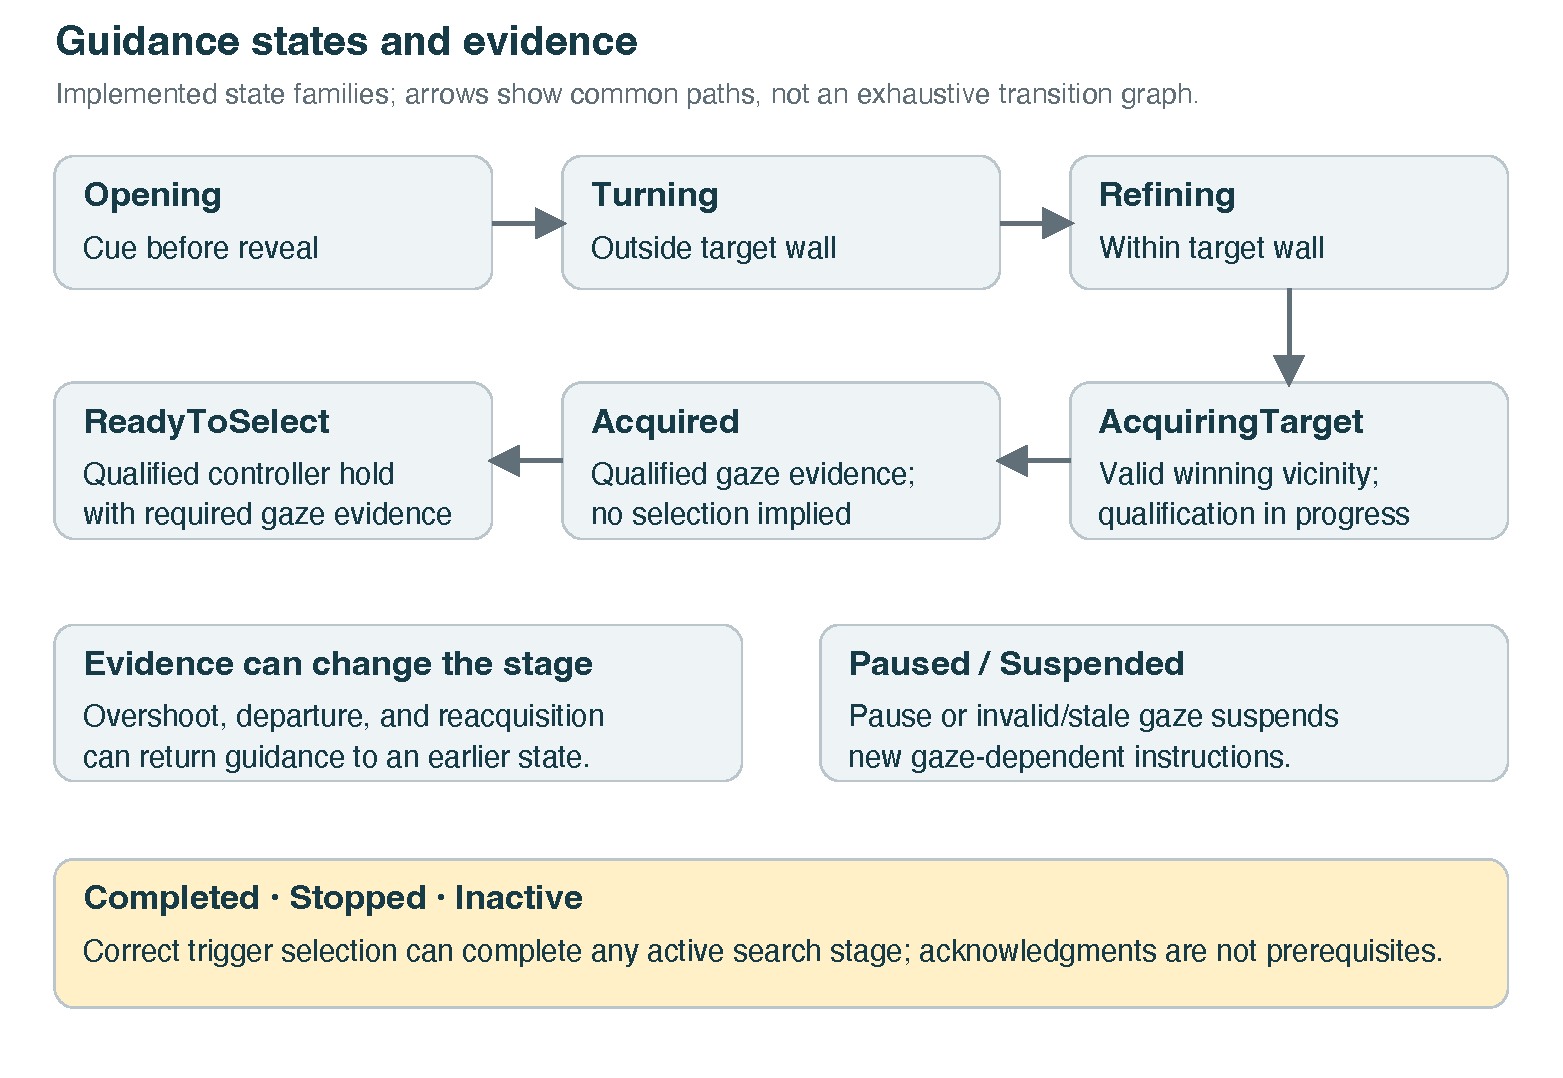
\includegraphics[width=\linewidth,alt={Common path from opening through turning and refinement to acquisition and readiness, with pause and suspension and independent trigger completion.}]{figures/guidance-states.pdf}
\caption[Guidance states and evidence-dependent transitions]{Implemented guidance state families. Turning, refining, acquisition, and readiness are evidence-dependent interpretations. Tracking loss, pauses, target departure, and reacquisition can change the path. Trial completion remains owned by the round manager.}
\label{fig:guidance-states}
\end{figure}


\section{A Worked Guidance Sequence}
Consider an illustrative target near the wall opposite the starting cross, with a rightward offset or the documented backward-turn tie rule. The opening cue may say that the object is to the right while objects remain hidden. Once search begins, progress cues can acknowledge continued rightward turning. On stable entry to the target wall, assistance can move to within-wall refinement, such as looking lower and slightly left. The reference for that refinement must be the recorded gaze geometry and local target relation, not a neighboring object's apparent screen position.

If the participant passes the target, recent spatial history can support a return cue. If the participant instead looks near the target long enough, a gaze acknowledgment becomes eligible. If the controller is already intersecting the target, away-directions are suppressed immediately. A qualified pointing acknowledgment can then identify controller evidence, and a right-trigger press can complete the trial. This example illustrates intended transitions; it is not a measured trajectory or evidence that all people follow this sequence.

\section{Asynchronous Decisions and Cancellation}
Each cloud request receives a snapshot, not a live reference to mutable state. The snapshot includes current evidence, relevant geometry, speech status, and bounded recent history. A response can become stale because the participant moves, tracking changes, the voice changes, a pause begins, or the trial ends. The scheduler checks those conditions again before playing the chosen clip. A valid answer to an old question is not necessarily a valid instruction now.

Prepared audio removes synthesis from the immediate hint path, but does not remove network latency from cloud choice. Time-sensitive qualified feedback can use local admission without waiting for another Jev decision. Ordinary hints can wait for phrasing choice within bounded scheduling rules. Interruption policy balances urgency against comprehensibility; finishing a short useful phrase may be preferable to cutting it at an awkward boundary. The documented implementation uses a 150-ms fade as a playback technique, not a guarantee of natural conversation.

Experimental policies that allow Jev broader action choice must be versioned separately from the participant policy. Replaying the same observations through multiple policies can compare decision latency and admissibility. It cannot show how a participant would have moved after hearing a different cue. The participant release will need one frozen policy and a manifest of thresholds, phrase library, Jev provider/model identifier, version and available sampling settings. Whether the provider sees voice-condition identifiers must be verified against the frozen payload; this draft does not assume condition-blind decisions. That audit will distinguish voice-related cancellation keys from information actually transmitted to the provider.

\chapter{USER STUDY METHODOLOGY}
\label{ch:study}
This chapter describes the within-participant user study that uses Follow My Voice to answer the research questions in Section~\ref{sec:research-questions}. It covers the experimental design and participants, the procedure, the data the system records, how each measure is scored, and the planned statistical analysis.

The study design draws on Chiossi et al.'s visual-search study, which combines search outcomes with eye-tracking measures~\cite{chiossi2024searching}. This study keeps that separation between task performance and visual behavior but changes the research question to voice identity, initially withholds the target identity, and uses a researcher-selected 25-second search limit. Complementary work by Pfeil et al. at UCF compares eye--head coordination in virtual and physical viewing~\cite{pfeil2018eyehead}. That work motivates retaining head motion alongside eye direction when interpreting gaze in this application.

\section{Experimental Design}
\label{ch:methodology}
\draftnote{This section specifies the proposed confirmatory procedure. The implemented snapshot supports one practice trial, two 40-trial blocks, and a final questionnaire handoff. It also records pre-cue starting geometry and balances target direction and height within each block. Sample size and pilot acceptance rules remain unresolved.}
\subsection{Voice Manipulation and Comparison Rationale}
This thesis compares two ways of personalizing assistance: a synthetic voice derived from the participant's recorded speech and a neutral voice selected by that participant from the supplied catalog. Letting participants choose the neutral alternative ties the comparison to a design choice a user could face. The within-participant task provides repeated observations under both configurations. Similarity ratings indicate whether participants heard the clone as resembling themselves, whereas performance and experience measures compare how each voice functions as guidance.

Gaze contingency and the agent's decision rules are common to both conditions. Because the target identity is initially hidden, participants receive repeated guidance in the assigned voice on every trial. Jev, memory, and gaze awareness are held constant rather than varied as independent factors.

\subsection{Design and Trial Allocation}
The study uses a within-participant comparison of two voice conditions: a neutral voice and a self-similar synthetic voice. Both conditions use the same guidance policy, semantic phrase library, selection method and visual-feedback settings, although actual phrase sequences may differ because guidance responds to behavior. Because the neutral voice is chosen by the participant whereas the clone is derived from the participant's speech, the two voices may also differ in preference, gender presentation and synthesis quality. The contrast therefore cannot isolate self-similarity from these features.

A saved, balanced randomized allocation assigns neutral-first or self-similar-first order. Counterbalancing the order distributes possible carryover from the first block across the two voices~\cite{williams1949residual}, although it does not remove carryover. Each participant completes one practice trial followed by two measured blocks of 40 trials, one per voice. The practice trial uses the first voice in the assigned order (the neutral voice for Order A, or the self-similar voice for Order B) and is excluded from measured outcomes. A seed makes the trial schedule reproducible. Nominal horizontal-angle quotas are identical across blocks, with trial order and left/right assignments randomized subject to those quotas. Within each block, each bilateral angle category (45, 90 and 135 degrees) has four left and four right assignments.

\begin{table}[htbp]\centering
\caption[Study allocation]{Study allocation. Nominal wall angles are schedule categories, not exact object bearings or accumulated head rotation.}
\tagpdfsetup{table/header-rows={1}}
\begin{tabularx}{\linewidth}{@{}lX@{}}\toprule
Parameter & Allocation \\\midrule
Voice conditions & Neutral voice; self-similar synthetic voice \\
Measured trials & 40 per block; 80 per participant \\
Practice & One trial; excluded from outcomes \\
Absolute nominal wall step & Eight trials each at 0, 45, 90, 135 and 180 degrees per block \\
Vertical allocation & 20 targets above and 20 below readiness-cross height per block; four above and four below at each nominal angle \\
Condition order & Counterbalanced neutral-first and self-similar-first \\
Active search limit & 25 seconds, excluding explicit pauses \\
Selection & Right-controller ray and a trigger press \\\bottomrule
\end{tabularx}
\end{table}

Objects vary in position within each plane of the shared layout, so each trial specifies the exact starting angle and target height in addition to the assigned wall. Vertical allocation is defined by target-center height relative to the readiness cross rather than the participant's seated eye height. The cross is placed at the midpoint of the permitted object-height range, and each assigned target center lies between 10 and 45 percent of that range above or below it. The lower bound keeps every target clearly above or below the cross, and the upper bound keeps targets away from the floor and the top of the wall. Pilot sessions will assess target visibility and seated comfort at both extremes.

\begin{figure}[htbp]\centering
\IfFileExists{figures/study-procedure-current.pdf}{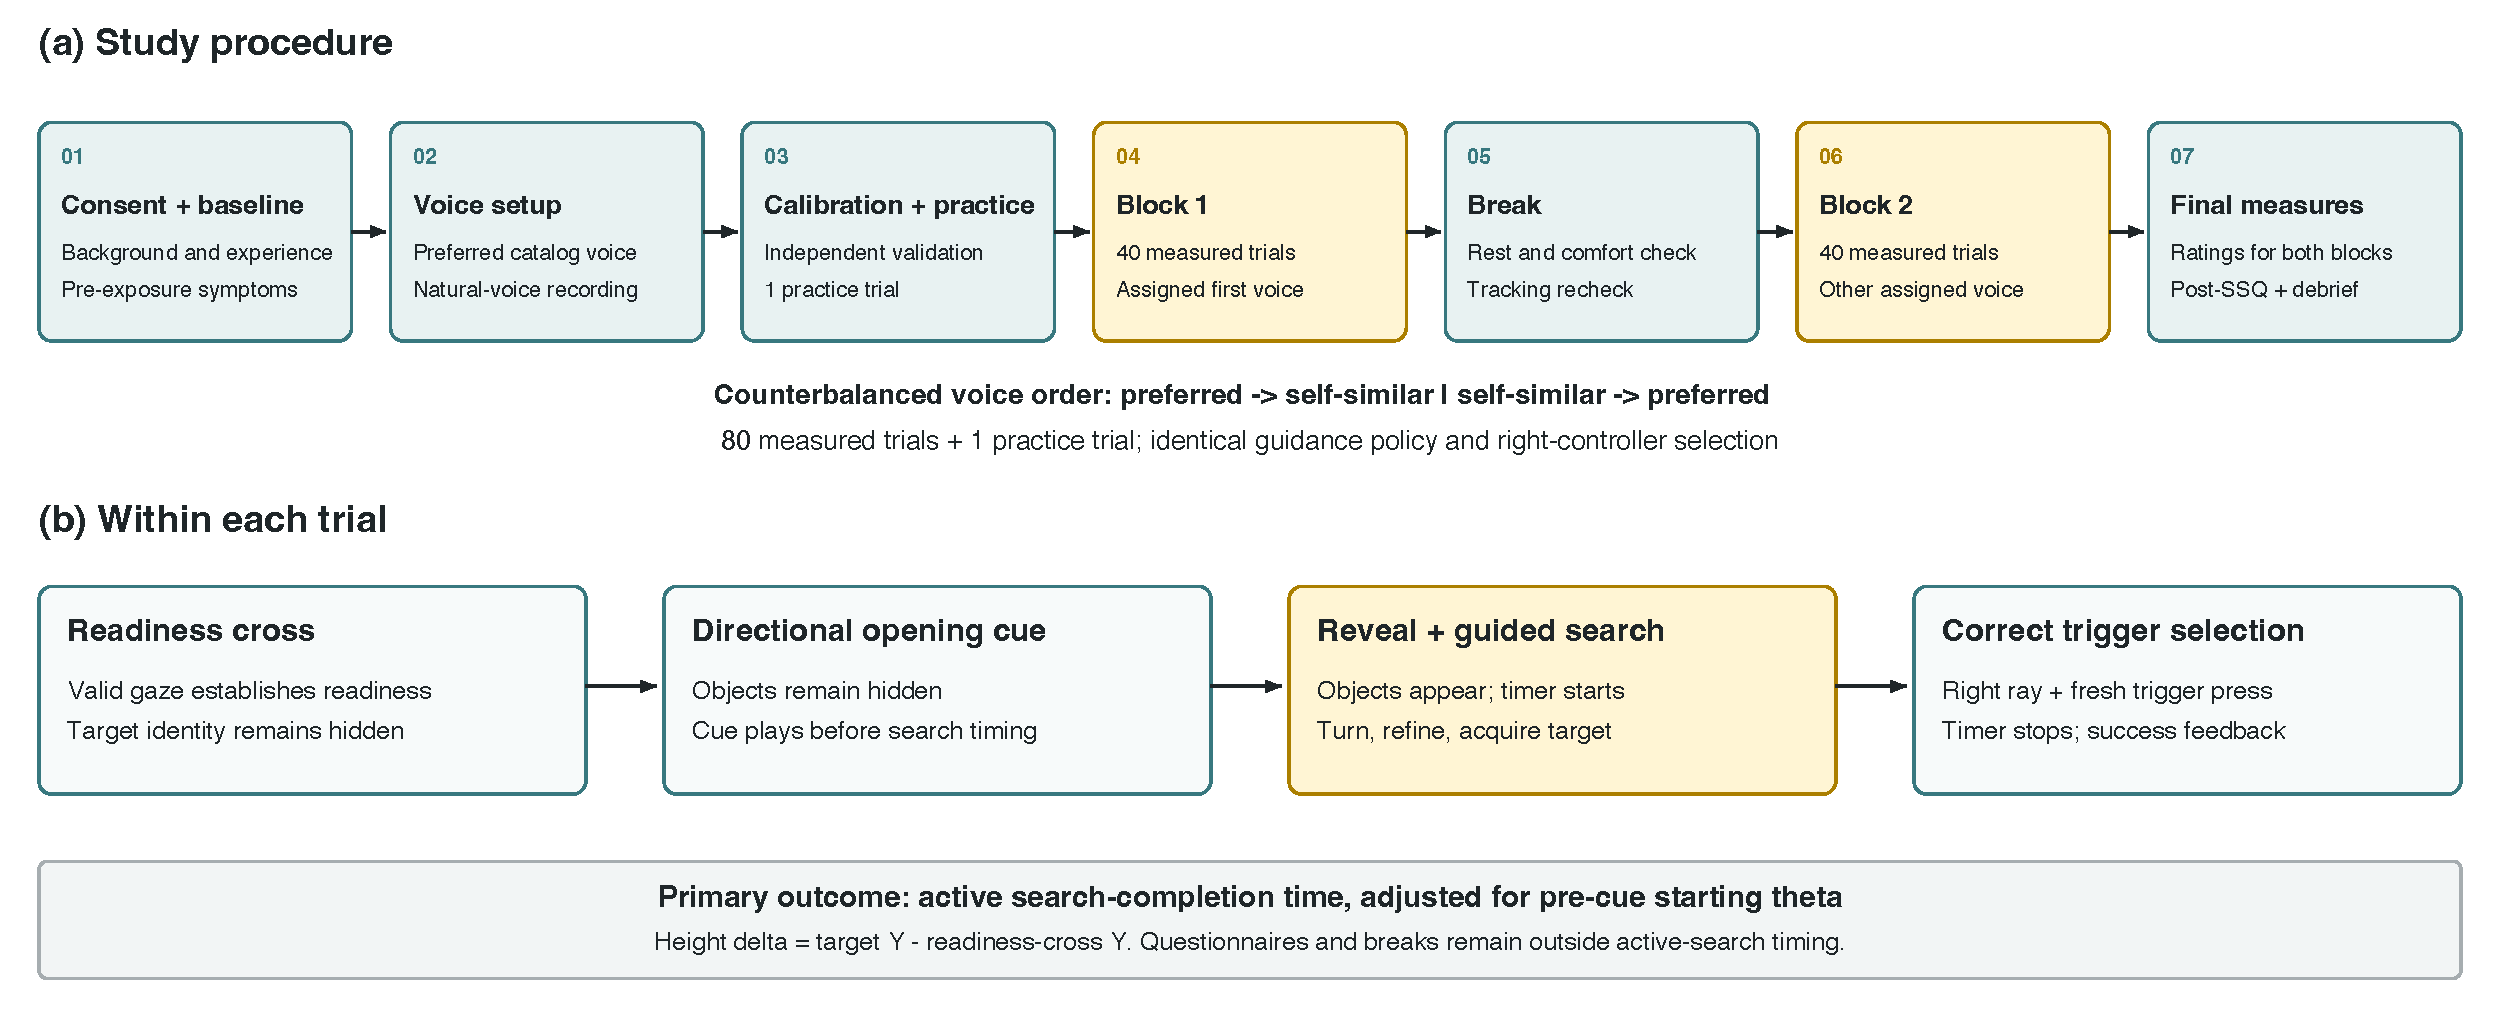
\includegraphics[width=\linewidth,alt={Setup and one practice trial precede two counterbalanced forty-trial blocks and final retrospective questionnaires; each trial separates opening cue, reveal, and trigger selection.}]{figures/study-procedure-current.pdf}}{\fbox{\parbox{0.94\linewidth}{Consent and setup $\rightarrow$ calibration and practice $\rightarrow$ 40-trial voice block $\rightarrow$ break $\rightarrow$ 40-trial voice block $\rightarrow$ survey and debrief. Within each trial: readiness cross $\rightarrow$ opening cue $\rightarrow$ object reveal and active search $\rightarrow$ correct trigger selection.}}}
\caption[Study procedure and trial timing]{Study procedure and trial timing. Opening guidance precedes object reveal; active completion time ends at correct right-trigger selection. The success path shown here is bounded by a 25-second active-search deadline; expiry ends the attempt without a successful completion time. Questionnaires and between-trial breaks remain outside active-search timing.}
\label{fig:study-procedure}
\end{figure}

\clearpage
Nominal angle steps are defined relative to the readiness (start) wall, which is the previous target wall. For the first measured trial, this reference is the practice target wall. The first measured cross is centered on its wall. Each later cross is shifted sideways by a seeded offset of up to 20 percent of the usable half-width. Target placement happens when readiness completes, while all objects remain hidden and before the opening cue. At that moment, the application rotates the horizontal bearing from the participant's eye origin to the cross by the assigned signed angle, places the target where that bearing meets the assigned wall, and arranges the remaining objects around it. The exact starting angle defined below therefore equals the assigned category at that instant. If the required position falls outside the wall, the session stops so the participant can recenter, rather than substituting a different angle or trial. Final positions depend on the saved eye origin as well as the seed, so each layout is reconstructed from the saved object positions.

\subsection{Participants}
Eligible participants are consenting adults able to understand the task, hear the guidance, view the scene with usual correction and safely use the seated setup and right controller. Handedness, visual correction and prior XR and voice-assistant experience are recorded. Sample size and the enrollment ceiling will be determined before recruitment by a power analysis for the theta-adjusted repeated-measures outcome that accounts for plausible within-participant variation and incomplete observations.

\subsection{Research Questions and Outcomes}
Each research question in Section~\ref{sec:research-questions} maps onto specific outcomes. RQ1 uses active completion time as the primary outcome, with missed targets and perceived workload, measured with an adaptation of NASA-TLX~\cite{hart1988nasatlx}, as secondary outcomes. RQ2 uses the Index of Pupillary Activity~\cite{duchowski2018ipa}, fixation count, and saccade frequency, which remain exploratory until the eye-event detectors are validated on the headset. RQ3 uses the interest/enjoyment subscale of the Intrinsic Motivation Inventory (IMI)~\cite{ryan1982control,mcauley1989imi}, with the other three IMI subscales reported alongside it. Agent perception, eeriness, voice experience, reliance, search behavior, and variation in the voice contrast with starting angle are exploratory. The hypotheses are directional, favoring the self-similar voice, but the voice contrasts are tested two-sided so that an advantage for the neutral voice would also be detected. Repeated trials are treated as within-participant observations, not as independent participants.


\section{Procedure}
Participants perform an agent-guided object-search task while seated on a swivel chair, with multiple colored geometric objects scattered across eight surrounding vertical planes. Although the application knows the target identity, the participant does not receive a color-and-shape description before searching. Instead, the agent guides the participant toward the target wall and then refines the direction horizontally, vertically or diagonally. The participant selects an object using the right-controller ray and trigger. Looking at an object, receiving a gaze confirmation or pointing at it does not by itself complete the trial.

Each trial begins with the participant looking at a readiness cross. Once readiness is established, an opening directional cue plays while the objects remain hidden, and object reveal then starts active search timing. A correct trigger selection before the 25-second active-search deadline stops timing and produces success feedback. An incorrect selection is counted, and search continues within that same limit.

If the target has not been selected after 25 seconds of active search, the trial ends as a timeout. The application hides the objects, cancels pending spatial hints, and plays a prepared encouragement in the assigned voice, beginning with ``Time up,'' before presenting the next readiness cross. For example, the agent may say, ``Time up. Let's shake that round off and start the next.'' Separate wording introduces the block break or acknowledges the final trial. The same deadline and phrase set apply to both voice conditions and to the single practice trial. A timeout advances the scheduled attempt without adding a replacement. Explicit pauses suspend the clock, whereas tracking loss alone does not. The 25-second limit is a researcher-selected protocol parameter, not a threshold drawn from the cited studies.

Before participant use, consent materials will be updated to describe ElevenLabs voice processing and Jev cloud decisions, including the data transmitted, retention, access, and deletion arrangements. After consent, participants complete background questions. They then choose a neutral voice, rate auditioned voices, record a standard passage in their natural voice for synthesis, and confirm comfortable, clear audio for each condition. The English recording passage is reproduced in Appendix~\ref{app:instruments}; its correspondence to the study build and its typical recording duration have not yet been verified. The neutral voice is chosen explicitly rather than inferred from participant gender.

The researcher fits the headset and conducts vendor calibration followed by independent spatial validation across relevant heights, wall boundaries, distances and head orientations. If an offset correction is introduced, the targets used to fit it are kept separate from those used for independent validation. Standardized instructions explain that participants rely on the agent to discover the target and use the right trigger to select it. Participants then complete the single practice trial and the two assigned 40-trial blocks.

No questionnaire interrupts the block sequence. Instead, during the final survey the same condition-specific questionnaire is completed twice, once referring to Block 1 and once to Block 2, with identical item wording and order. Breaks are offered between trials and at the block boundary, and any necessary in-trial pause is logged immediately. Tracking is rechecked between blocks and after headset adjustment. After headset removal, participants complete the two retrospective condition-specific sets, comparative voice preference and debrief. Participants may request a pause or stop, and symptoms or technical problems prompt researcher assessment.

Figure~\ref{fig:survey-scopes} distinguishes administration time from reference scope: both condition-specific batteries are completed in the final session, but each response refers to a single measured block.

\begin{figure}[htbp]
\centering
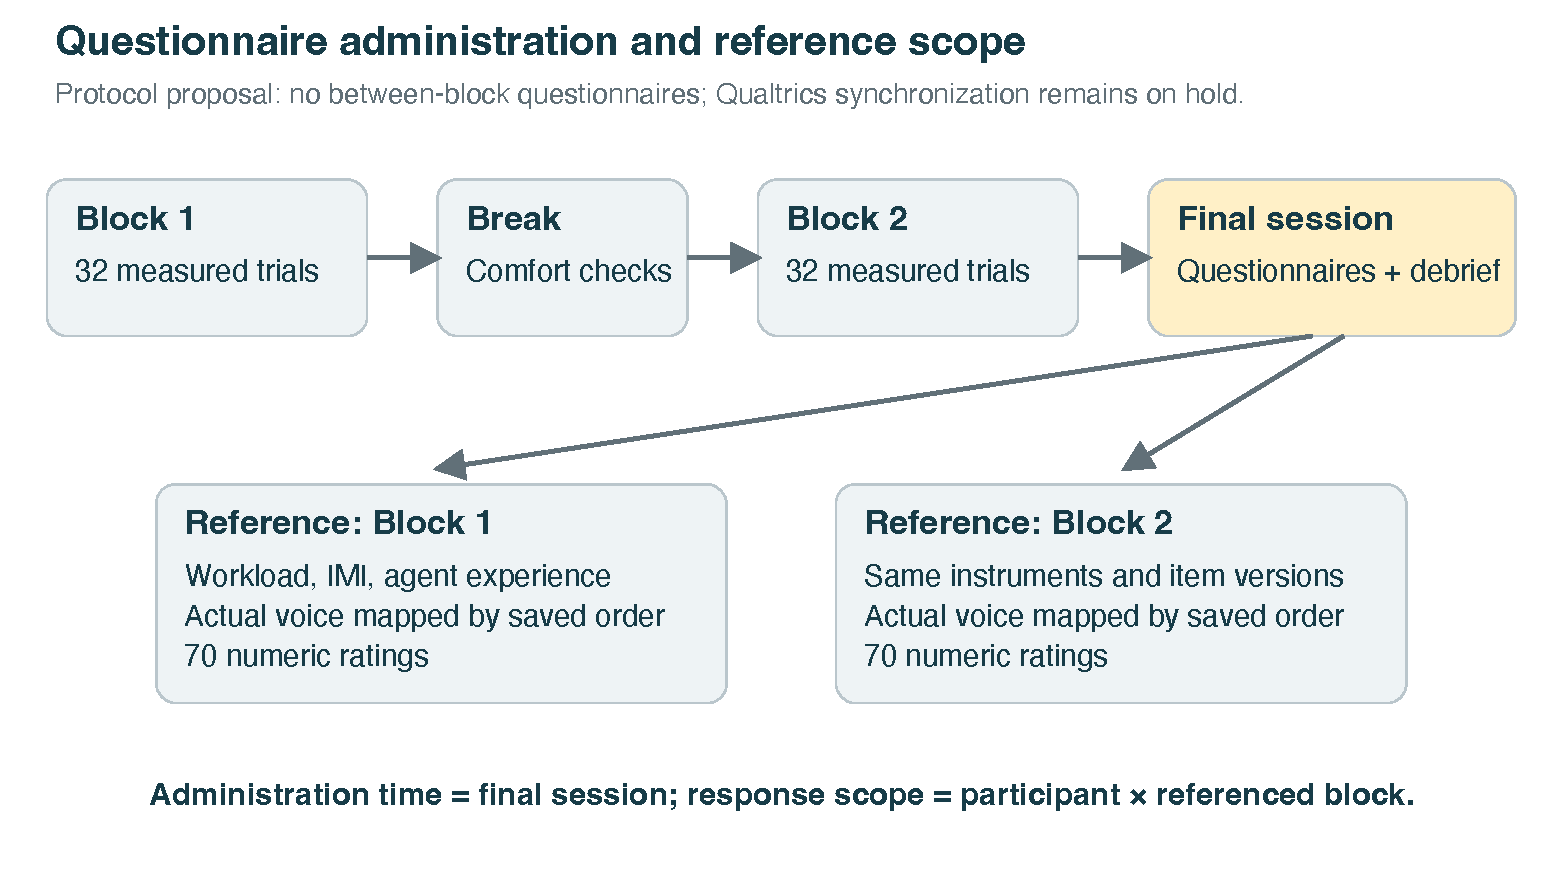
\includegraphics[width=\linewidth,alt={Two blocks separated by a break are followed by a final session with questionnaires referring separately to Block 1 and Block 2.}]{figures/survey-scopes.pdf}
\caption[Final questionnaire timing and block reference scope]{Proposed final retrospective administration. The intervening break contains comfort and tracking checks, not a block questionnaire. Each block-referenced battery contains 65 numeric ratings. Actual voice is recovered from the saved counterbalanced order.}
\label{fig:survey-scopes}
\end{figure}


The final survey will include an unambiguous reminder linking each block reference to the voice heard in that block. The reminder format (such as neutral labels or replayed samples) has not yet been decided and will be piloted to check that it adds no differential cues between conditions.

\subsection{Pilot Testing and Parameter Checks}
Before confirmatory recruitment, pilot sessions verify the realized angle/height schedules, target visibility and seated comfort, readiness and selection behavior, gaze validity, audio timing and wording, and reconstruction of trial events from the saved data. Pilot assessment also measures survey comprehension and completion time. These checks inform calibration-acceptance, practice-proficiency and technical-stop criteria. The pilot also assesses whether the 25-second deadline is suitable, and the outcome is documented with the study build and questionnaire versions.

\section{Data Collection}
\label{ch:measurement}
Measuring the voice comparison involves three questions: whether participants perceived the self-similar voice as resembling their own, whether voice condition changed search performance, and how participants experienced the assistance. Answering them requires outcome measures together with an account of the speech each participant actually heard. This section therefore links voice identity, delivered speech, search events, and questionnaire responses, so that perceived similarity can be reported as a manipulation check and kept distinct from performance and experience outcomes. Detailed gaze and timing records support interpretation of these outcomes, and Appendix~\ref{app:instruments} retains instrument wording and scoring.


\subsection{Frame-Level Records and the Trial CSV}
The recording separates time-varying observations from trial summaries. Frame records retain application time, gaze origin and direction with tracking validity, head pose, available controller poses and input state, and the gaze/controller object-intersection evidence used by guidance. Object identities and transforms provide the scene needed for reconstruction; guidance transitions, agent decisions, actual speech playback, trigger selections, and pauses are recorded as events. A rendered frame can reuse a sensor observation, so frame count must not be reported as the number of independent eye-tracking samples.

For new rotational-search recordings, the trial replay snapshot additionally stores the wall bottom in recording-local coordinates, the wall height in metres, and a flag indicating that these bounds are available. Trial Review uses those recorded bounds to reconstruct the shorter walls. Earlier recordings without explicit bounds retain object-derived wall estimates and their original object positions; they are not rescaled to the current layout. These replay fields supplement the layout version and saved transforms and are distinct from the columns in the trial CSV. Analyses that include recordings from both layouts must retain that provenance rather than treat the geometry as unchanged.

Trial Review generates an Excel-compatible trial CSV with one row per trial. Its fields describe task performance, geometry, guidance exposure, and associated subjective responses (Table~\ref{tab:trial-fields}). Outcome, practice, provenance, and quality information accompany the exported records to support analysis and eligibility checks.

\begin{table}[htbp]\centering
\caption[Trial CSV contents]{Contents of the trial CSV. Unavailable values remain blank; reserved fields do not imply that a measure has been collected.}
\label{tab:trial-fields}
\small\tagpdfsetup{table/header-rows={1}}
\begin{tabularx}{\linewidth}{@{}p{0.23\linewidth}X@{}}\toprule
Group & Recorded or derived columns \\\midrule
Identity & Participant ID, trial ID, block index, voice condition. \\
Geometry & Absolute and signed nominal theta; actual signed head-to-target yaw; target-minus-head height; target distance. \\
Guidance and duration & Instruction count and search exposure in seconds. \\
Target contact & Time to first and final target gaze contact; first right-controller target contact; final selection. \\
Subjective context & NASA-TLX score; reserved subjective performance rating, currently blank pending an agreed instrument mapping. \\\bottomrule
\end{tabularx}
\end{table}

The export's post-onset head-relative yaw and height must not be relabeled as the proposed pre-cue cross-relative geometry. Gaze-contact times describe ray intersections, not validated fixations. A block-referenced questionnaire score may appear on multiple trial rows for convenience, but remains one block-level observation.

\subsection{From Interaction Events to Research Variables}
The recorded data serve two purposes: reconstructing what happened in a trial and estimating the study outcomes. Reconstruction requires observations and events at their original temporal resolution, whereas statistical analysis usually requires a more compact table. The project therefore keeps trial summaries separate from gaze, head/controller motion, object layouts, and event streams, treating each summary as a derived representation rather than a replacement for the underlying evidence.

Every derived value needs an identifiable source and a definition. A number called ``time to gaze'' is ambiguous unless it specifies the clock origin, the contact rule, validity handling, and the treatment of missing observations. The data contract preserves these meanings in separate fields.

Figure~\ref{fig:data-provenance} shows how a trial CSV remains linked to the underlying observations, so that values prepared for statistical analysis can still be traced to the records needed for trial reconstruction.

\begin{figure}[htbp]
\centering
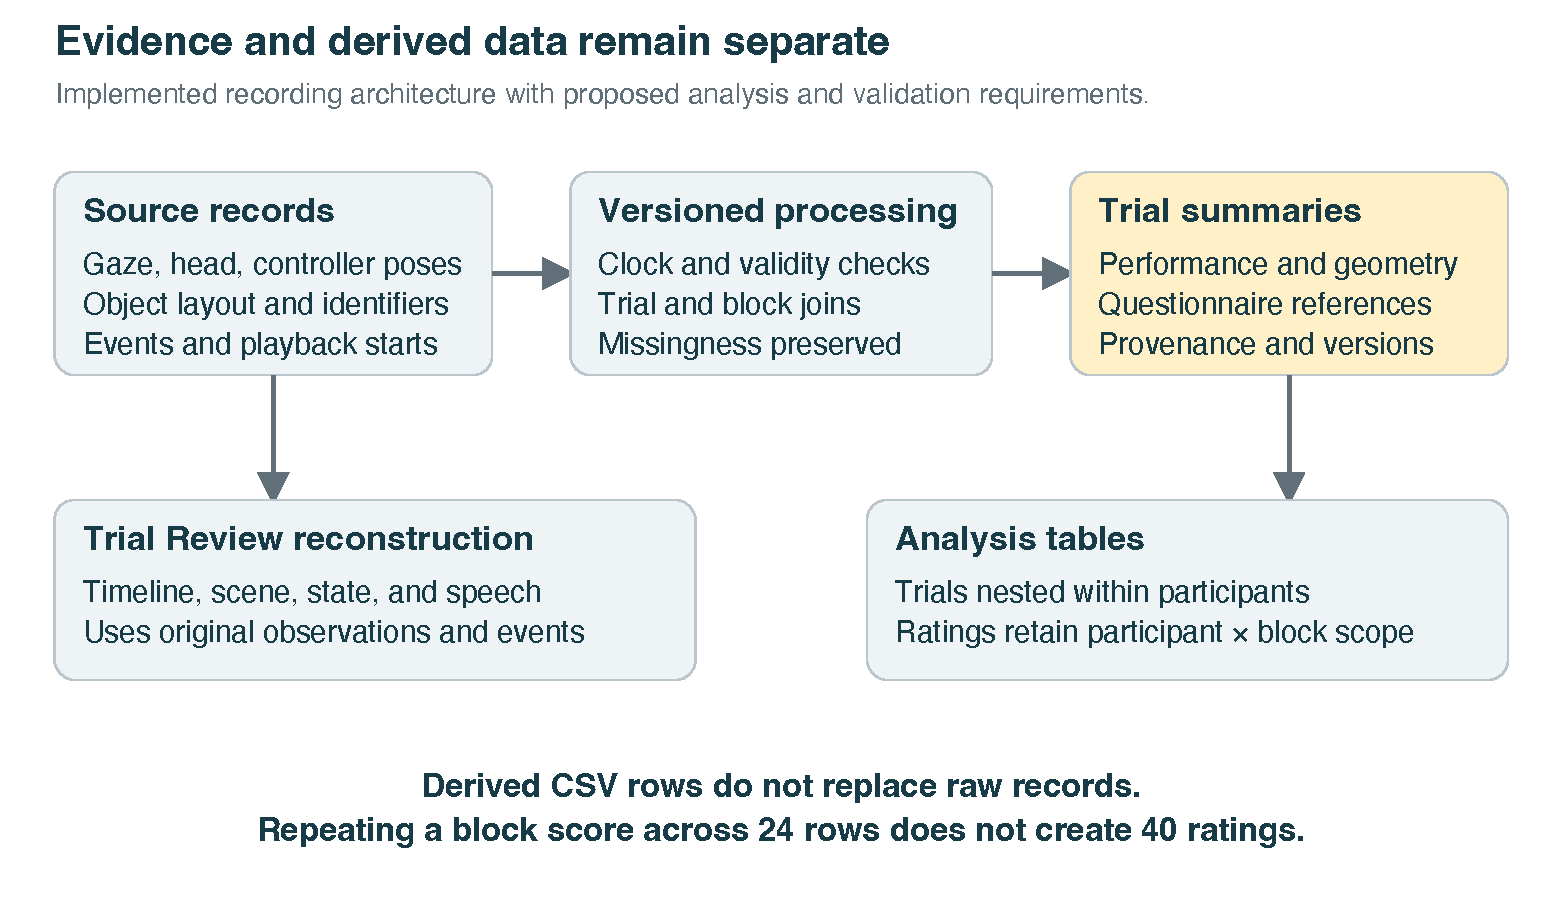
\includegraphics[width=\linewidth,alt={Raw observations and events feed versioned processing, trial summaries, Trial Review, and analysis tables.}]{figures/data-provenance.pdf}
\caption[Raw records, derived summaries, and analytical scope]{Recording and processing relationships. Source streams support reconstruction; derived summaries support analysis. Processing and scoring require versioned definitions. Repeating block-level ratings in trial rows does not create new independent observations.}
\label{fig:data-provenance}
\end{figure}


\subsection{Coordinate Frames and Starting Geometry}
Let $\mathbf{o}$ denote the saved trial reference origin, $\mathbf{c}$ the readiness-cross center, and $\mathbf{p}$ the target center. All three positions must be expressed in the same world coordinate frame. Let $\Pi(\mathbf{v})=(v_x,0,v_z)$ project a vector onto the horizontal plane. Define
\begin{equation}
\mathbf{a}=\Pi(\mathbf{c}-\mathbf{o}),\qquad
\mathbf{b}=\Pi(\mathbf{p}-\mathbf{o}).
\end{equation}
For nondegenerate vectors, the exact pre-cue starting angle is
\begin{equation}
\theta_0=\operatorname{atan2}\!\left(\hat{\mathbf{y}}\cdot(\mathbf{a}\times\mathbf{b}),\,\mathbf{a}\cdot\mathbf{b}\right)\frac{180}{\pi}.
\end{equation}
Verification compares the sign convention against Unity's world-up signed-angle convention using known left and right targets. The absolute value $|\theta_0|$ describes horizontal demand from the saved cross reference. Exactly backward targets require a documented tie convention, because $-180$ and $+180$ identify the same horizontal bearing, although the absolute magnitude remains 180 degrees in either case.

This calculation is a required addition to the frozen study data contract. The October 20, 2026 implementation alignment audit found that existing signed and absolute theta fields represented nominal wall geometry relative to the previous target wall. They must not be renamed or silently interpreted as exact pre-cue measurements. A new snapshot must save origin, cross, target, timestamp, frame, and coordinate-frame identifier before the opening cue. If a horizontal vector is degenerate, the angle is unavailable; substituting zero would falsely describe an easy starting configuration.

Nominal categories remain useful for allocation: each block contains eight scheduled trials in each absolute category, $0,45,90,135,180$ degrees. Because an object can be positioned away from the center of its assigned wall, however, its exact bearing need not equal the nominal category, and balance across categories therefore does not prove exact geometric matching between voice blocks. Both assigned and realized geometry are inspected.

The signed height difference is
\begin{equation}
\Delta h=p_y-c_y.
\end{equation}
Positive values identify targets above the cross center and negative values identify targets below it; this reference is not interchangeable with seated eye height. The planned 20-above/20-below allocation must be checked against realized positions and a prespecified near-zero rule, because the height scattering in the source snapshot did not enforce that balance.

The three-dimensional distance measure relies on a different observation: the first valid tracked head position $\mathbf{h}_k$ after reveal. Its value is $d=\|\mathbf{p}-\mathbf{h}_k\|_2$, in metres, and the timestamp of $\mathbf{h}_k$ must accompany the distance. Because this post-reveal measurement describes geometry at an observed head pose, it cannot recover an unrecorded pre-cue snapshot.

Figures~\ref{fig:starting-geometry} and~\ref{fig:height-reference} illustrate the proposed geometric contract using conceptual rather than recorded layouts.

\begin{figure}[htbp]
\centering
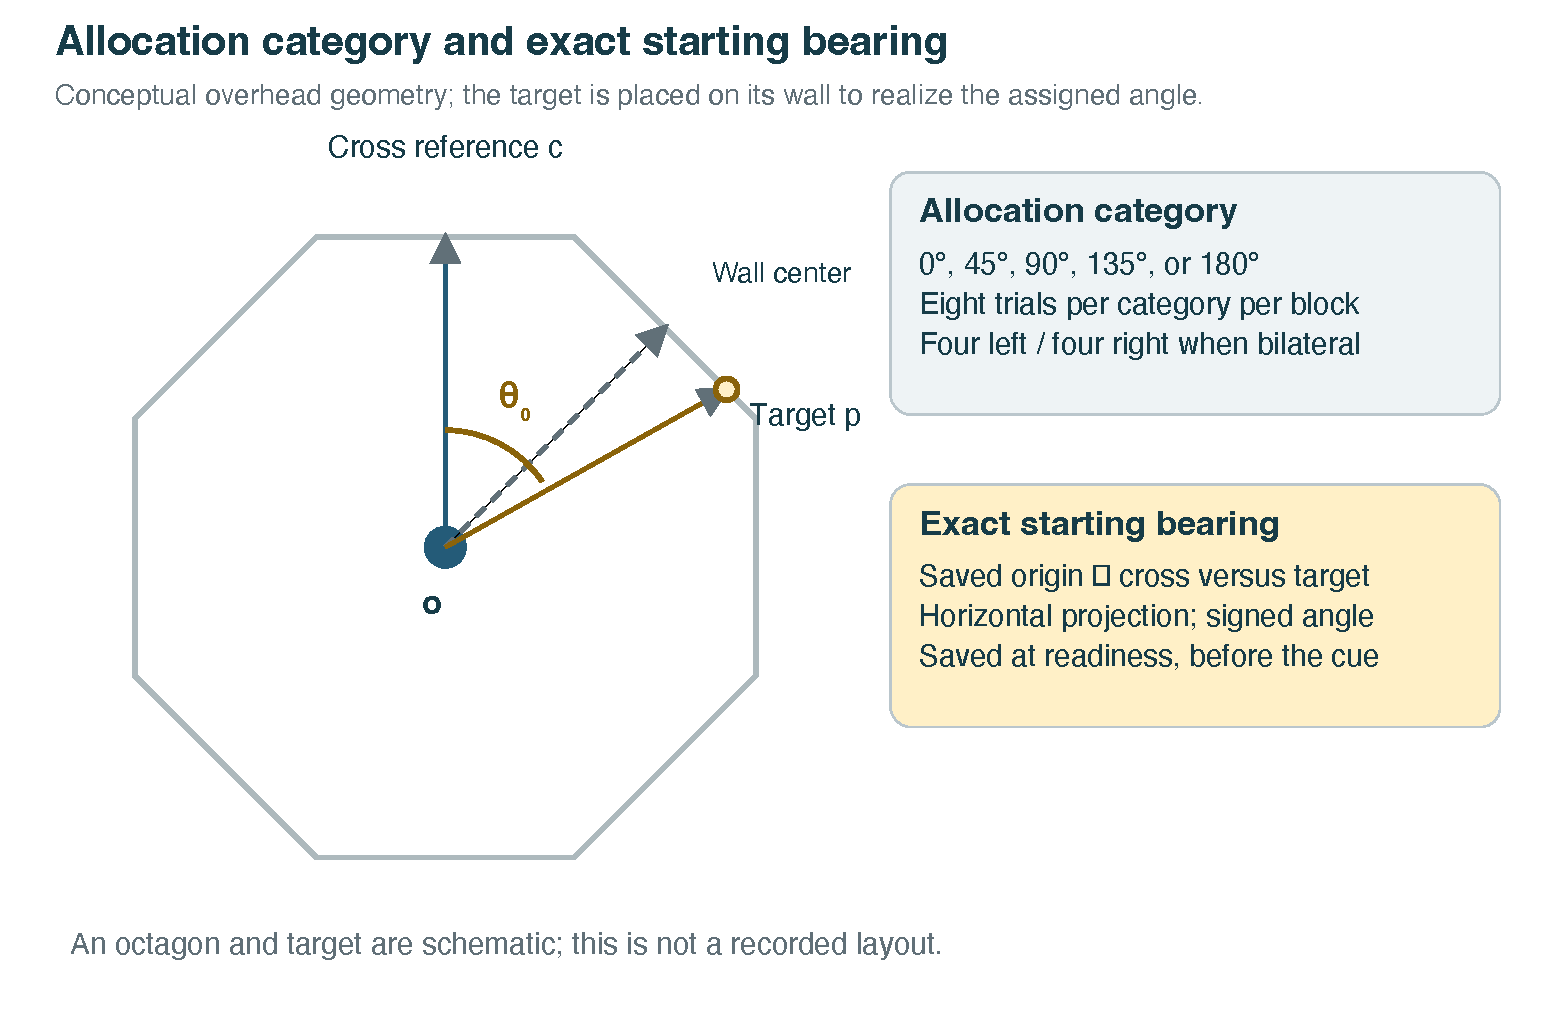
\includegraphics[width=\linewidth,alt={Overhead octagonal layout with origin, cross reference, nominal wall center, and an offset target showing distinct bearings.}]{figures/starting-geometry.pdf}
\caption[Nominal wall assignment and exact starting angle]{Conceptual overhead geometry. The target can be offset from its wall center, so an allocation category need not equal the realized starting bearing. The exact pre-cue snapshot remains an implementation requirement at the aligned checkpoint.}
\label{fig:starting-geometry}
\end{figure}


\begin{figure}[htbp]
\centering
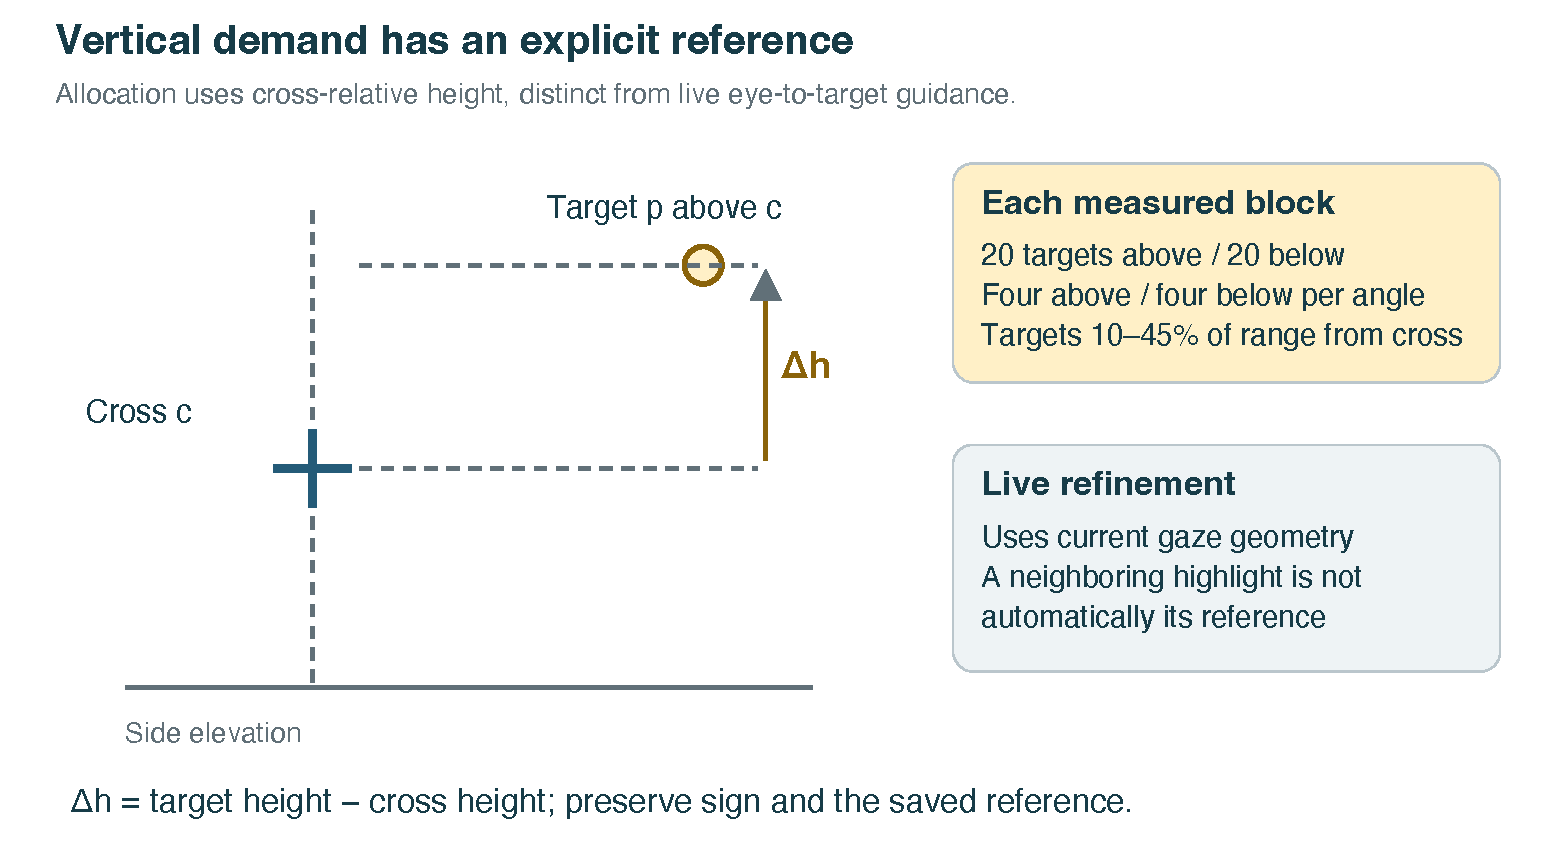
\includegraphics[width=\linewidth,alt={Side elevation of cross and target with positive signed height difference and a distinction between allocation and live refinement.}]{figures/height-reference.pdf}
\caption[Cross-relative height and live gaze refinement]{Conceptual side elevation for the proposed signed height difference. The target shown above the cross has positive height delta. The planned above/below quota and near-zero rule remain unresolved implementation and protocol checks; live vertical guidance uses current gaze geometry.}
\label{fig:height-reference}
\end{figure}


\subsection{Trial Clocks and Pause Intervals}
Let $t_r$ be object reveal, $t_s$ correct selection, and $\mathcal{P}$ the union of valid pause intervals. Active completion time is
\begin{equation}
T_{\mathrm{active}}=(t_s-t_r)-\mu\!\left([t_r,t_s]\cap\mathcal{P}\right),
\end{equation}
where $\mu$ denotes elapsed duration. Using the union prevents overlapping pause reasons, such as an application-focus pause that coincides with a researcher-requested pause, from being subtracted twice. The active clock remains stopped until every relevant pause reason has been resolved.

Readiness and opening speech precede reveal and are deliberately excluded from active search time. The measurement specification also includes the broader interval from opening-cue onset to selection. This measure includes the opening instruction, whose duration may differ across voices, while active completion time remains the primary outcome.

A stopped or timed-out trial has an observed duration and an outcome reason, but it does not have a successful completion time, and the analysis must not copy its stop timestamp into a success field. In the October 23 deadline implementation, a timeout records 25 seconds of active search exposure, a distinct timeout event, and an unsuccessful outcome. Software observes expiry on an update, while the exposure clock is capped at the deadline; event timestamps retain the actual observation time. Earlier development recordings retain their original durations and must not be retrospectively truncated to this limit. Source and receipt timestamps are likewise kept distinct, because a file that arrives late in the viewer reflects a transfer delay rather than necessarily a delay in the headset event.

Madritsch et al. distinguish overall task-completion time from active working time in an assistant-supported procedural task~\cite{madritsch2026assistance}, and their active measure is not assumed to correspond to the present clock. In Follow My Voice, active completion time includes ordinary waits for guidance between object reveal and correct selection, and only recorded pauses are excluded. Separate decision and playback timestamps help explain delivery delays without removing their task-level consequences from the primary outcome.

\subsection{Missed Targets}
A missed target is a search that reaches its recorded 25-second active-search deadline without a correct trigger selection. An incorrect selection followed by a correct selection before expiry is a completed search, with its selection error retained separately. Technical stops, withdrawal, and recordings without a known terminal outcome are not automatically classified as misses. For each participant, block, voice condition, and recorded deadline, the descriptive missed-target percentage is
\begin{equation}
M=100\frac{N_{\mathrm{timeout}}}{N_{\mathrm{selected}}+N_{\mathrm{timeout}}}.
\end{equation}
The denominator excludes practice and unresolved or technically interrupted attempts; their counts are reported alongside the percentage. A zero denominator yields an unavailable percentage. The full trial export implements \texttt{missed\_target} as 1 for timeout, 0 for successful completion, and blank otherwise. A separate \texttt{missed\_targets.csv} records grouped counts, deadlines, and development-data exclusion labels. Legacy records without an explicit deadline are retained but excluded from this deadline-specific percentage.

This outcome follows Chiossi et al.'s distinction between successful search and searches ending without selection~\cite{chiossi2024searching}. Their five-second task and the present 25-second, verbally guided task differ; percentages are therefore interpretable within each protocol and are not directly comparable benchmarks. The six unfinished searches in the earlier development recordings remain unfinished records, not retrospectively assigned missed targets.

\subsection{Eye-Event and Pupil Measures}
An implemented offline analysis preserves per-eye directions and pupil diameters from the HTC query stream, deduplicates repeated query timestamps, and separates search from readiness and pauses. Query receipts establish when software obtained data, not the sensor capture time or the independence of consecutive observations. Changes in trial or device, invalid tracking, reversed timestamps, and query gaps longer than 25 ms break continuity. Invalid per-eye observations and observed eye closure exclude nearby 200-ms intervals.

The fixation detector uses elapsed-time dispersion: the sum of horizontal and vertical angular ranges must remain within 1.8 degrees for at least 83 ms. This starting configuration follows the I-DT parameters reported by Chiossi et al.~\cite{chiossi2024searching}, within the detector family described by Salvucci and Goldberg~\cite{salvucci2000fixations}. Azimuth is unwrapped across the signed-angle boundary. The implementation retains event intervals and the duration of eligible segments; its counts are candidate classifications rather than validated fixations.

The saccade detector operates separately on eye-in-head angular velocity, with a provisional 60-degree-per-second threshold, a duration of 20--100 ms, at least two sampled intervals, and observed lower-velocity samples on either side. Intervals with head speed above 20 degrees per second or unavailable head pose are excluded. The reported rate divides event count by retained low-head-speed duration. It therefore describes a restricted observation window, not all saccades during search. These restrictions reduce head-turn ambiguity but do not validate event identity or establish sensor-level eye--head synchronization.

The Index of Pupillary Activity (IPA) calculation follows the wavelet-based approach of Duchowski et al.~\cite{duchowski2018ipa}. Each eye is processed separately. Accepted pupil segments contain valid finite diameters, last at least two seconds, meet a median query-rate screen of 60 Hz, and pass an interval-regularity screen. Within each accepted segment, values are resampled at its median query interval; no interpolation crosses rejected gaps or invalid observations. Level-two sym16 wavelet detail coefficients yield thresholded modulus maxima, which are counted per retained second. The implementation records its thresholds, resampling, numerical tolerance, and nearest-neighbor boundary convention. IPA is unavailable when no segment qualifies; it is never filled with zero to represent missing measurements.

Computational tests verify event boundaries, query deduplication, invalid-data handling, head-turn suppression, and wavelet calculations. They do not establish physiological validity. Independent event annotations, calibration checks, timing assessment, and held-out threshold evaluation remain necessary before fixation counts or saccade rates enter the participant analysis. Pupil-based interpretation additionally requires checks for luminance, gaze angle, blink artifacts, segment boundaries, and task-related confounds. IPA remains exploratory alongside NASA-TLX, rather than a validated estimate of workload in this apparatus. Final fixation duration on the target also remains unavailable until validated eye events can be joined to target areas of interest; the last ray contact is not a substitute.

\subsection{Gaze Contact, Vicinity, Pointing, and Selection}
Four event families are central to interpretation: a valid eye ray can intersect the target collider; a gaze direction can satisfy the larger target-vicinity rule; the right-controller ray can intersect the target; and a trigger press can select the target. These events can occur at different times and need not occur in that order in every recorded sample sequence.

The first gaze-contact latency uses the first valid recorded target-ray intersection after reveal. The last gaze-contact time uses the last such intersection before trial end. Neither is a fixation duration. If no contact is observed because of a blink, acquisition gap, or a path that only enters the broader vicinity, the contact field remains missing.

Vicinity qualification is an interaction rule rather than a fixation classifier. In the documented system, a target can be acknowledged after 100 ms of valid qualifying evidence, with overlapping regions resolved to a single closest candidate. The rule trades exact collider intersection for a tolerance intended to make feedback usable, but an overly large region can produce premature acknowledgment even when the timing gate behaves correctly. The tolerance must therefore be logged and piloted; its study-release value has not been frozen, and the default ring in the synthetic viewer screenshot is not a validated study setting.

Controller pointing is a distinct input observation, but its spoken acknowledgment is not independent of gaze: the documented rule requires a qualified one-second controller hold with valid gaze in the target vicinity when the speech scheduler permits the acknowledgment to play. Before the hold completes, a valid target hit already suppresses contradictory away-directions; this suppression prevents a direction such as ``go back down'' from being delivered while the controller is already on the target, without announcing that the hold has qualified. Correct trigger selection is the only event that successfully completes the search; a stop or timeout has a different outcome.

Figure~\ref{fig:evidence-events} contrasts the two acknowledgment events with trial completion.

\begin{figure}[htbp]
\centering
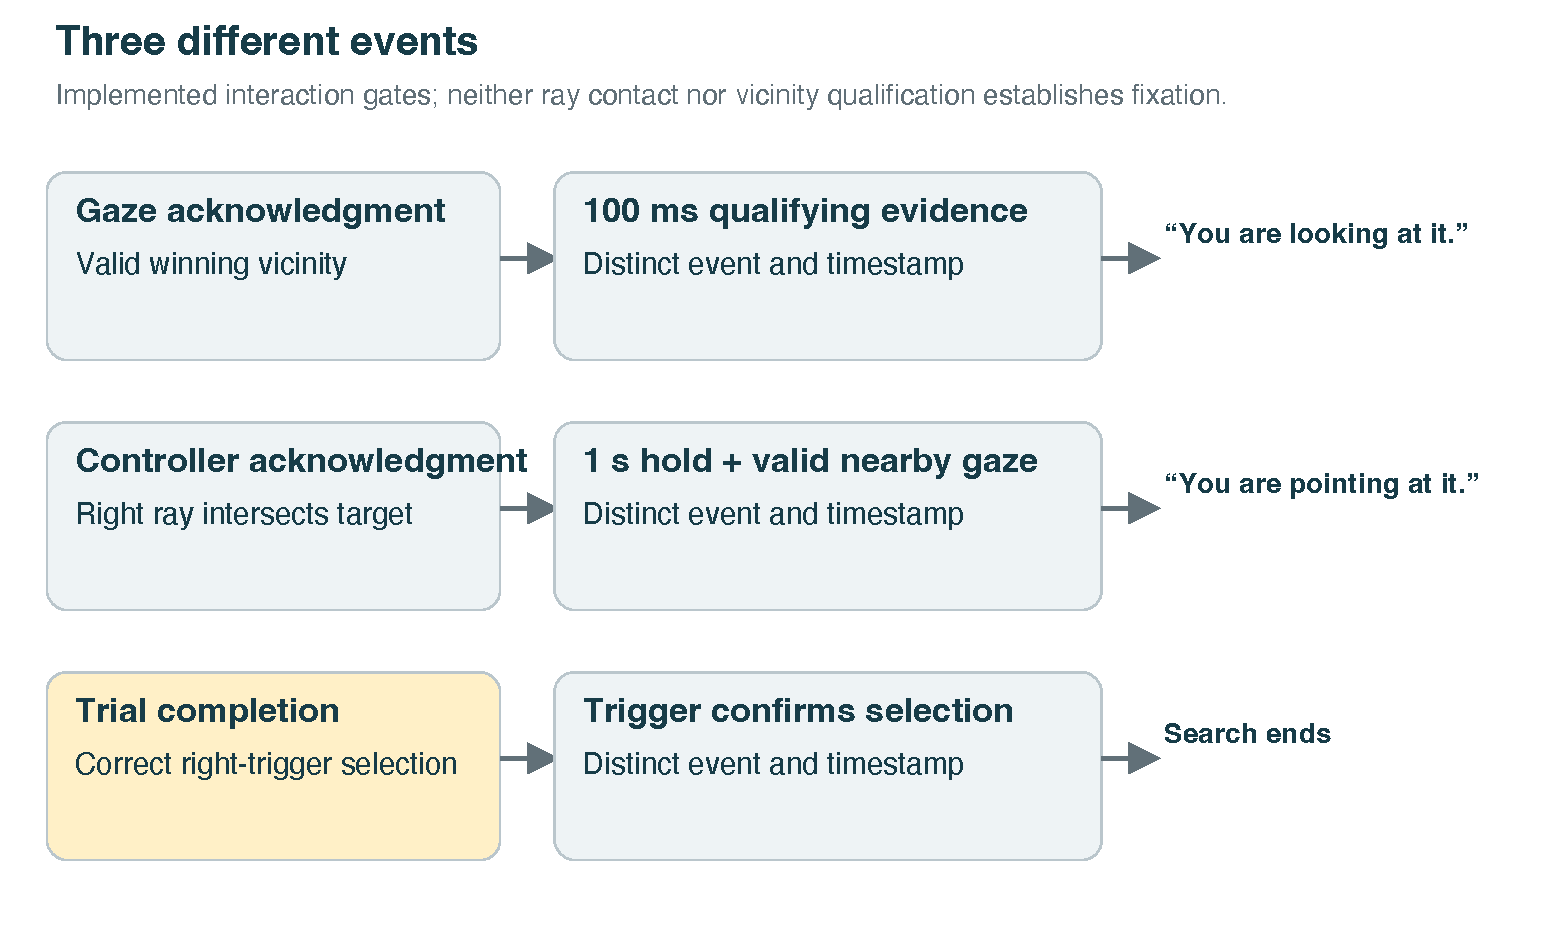
\includegraphics[width=\linewidth,alt={Three separate rows show qualified gaze, qualified controller pointing, and correct trigger selection as distinct events.}]{figures/evidence-events.pdf}
\caption[Gaze acknowledgment, pointing acknowledgment, and completion]{Implemented interaction distinctions. Gaze acknowledgment uses a 100-ms qualifying vicinity gate; pointing acknowledgment uses a one-second controller hold with required valid nearby gaze. A correct trigger selection completes the trial independently of whether either acknowledgment was spoken. These are interaction gates, not validated fixation measures.}
\label{fig:evidence-events}
\end{figure}


\subsection{Acquisition Rate, Validity, and Gaps}
A render loop can query an eye-tracking API frequently without receiving a new hardware observation each time, so the effective acquisition rate must be estimated from distinct source observations. If $n$ unique observations span source times $t_1$ through $t_n$, a basic rate summary is $(n-1)/(t_n-t_1)$. Because a mean alone can conceal bursty delivery, the distribution of successive intervals, repeated timestamps, invalid observations, and long gaps must accompany that average.

Application timestamps describe when data were handled, whereas source timestamps describe when the tracking observation was produced, if the API exposes them reliably. A clock-domain mapping must therefore be established before age or latency is computed across these clocks. If unique source timing is unavailable, the report states that limitation rather than infer 120-Hz binocular delivery from polling or headset specifications.

Spatial validation compares gaze direction with known independent targets. Angular error is computed from normalized gaze and expected target directions, with invalid observations excluded from the error distribution but retained in availability summaries. Precision and bias should be considered separately, since a stable offset and a noisy signal can produce different guidance failures even when their average angular error is similar. The validation procedure must also describe target exposure, head pose, corrective lenses, and headset adjustments.

\subsection{Motion, Coverage, and Instructions}
Gross translation sums Euclidean differences between adjacent valid head positions, and gross rotation sums shortest quaternion angular differences; invalid intervals, excessive gaps, and pauses break the accumulation. Gross movement is a total, not a rate. If a separate movement-rate outcome is derived, its denominator is observed covered time rather than the entire nominal session, because otherwise two runs with different data loss could produce misleadingly different movement rates.

Fixed-axis components derived from rotation vectors are not Euler yaw, pitch, and roll, and their labels retain the actual calculation. Head motion also does not directly measure swivel-chair rotation, because the head can move relative to the torso and chair.

Instruction counts use actual software playback starts; a requested cue, a rejected model answer, and a prefetched clip are not delivered instructions. Opening cues, search guidance, acknowledgments, reminders, and success speech have separate categories. The planned total of delivered active-search assistance includes directional guidance, gaze/pointing acknowledgments, and selection reminders, with each category also reported separately, while opening and success speech remain outside that total. Interrupted speech counts as started speech but retains its completion status, so it should not be treated as if the participant heard every word.

\subsection{Sequence-Level Latency}
For a qualified event, let $t_q$ denote the earliest supported qualification time and $t_p$ the actual software playback start of the corresponding acknowledgment. The primary engineering delay is
\begin{equation}
L_{\mathrm{software}}=t_p-t_q.
\end{equation}
This is not acoustic latency at the participant's ear, because audio-device buffering and the physical sound path require a separate measurement. Gaze and controller qualification times must also use their own definitions, since comparing a controller acknowledgment against first gaze contact would inflate or misattribute its delay.

Repeated requests about one continuously qualified event form a single episode, so a sequence can include several decisions by Jev to wait without creating several independent missed confirmations. An episode ends with playback, disqualification, trial termination, or a defined reset, and the evaluation reports how those endpoints were assigned, marking incomplete evidence as unknown.

Where logs support attribution, waiting is divided into model response, explicit model deferral, scheduling, existing speech, and audio readiness. Because these intervals may overlap, they are not summed unless they are represented as a nonoverlapping partition of the critical path. The full event timeline remains the authority when aggregate attribution is ambiguous.

Figure~\ref{fig:latency-definition} separates intentional evidence qualification from subsequent delivery delay.

\begin{figure}[htbp]
\centering
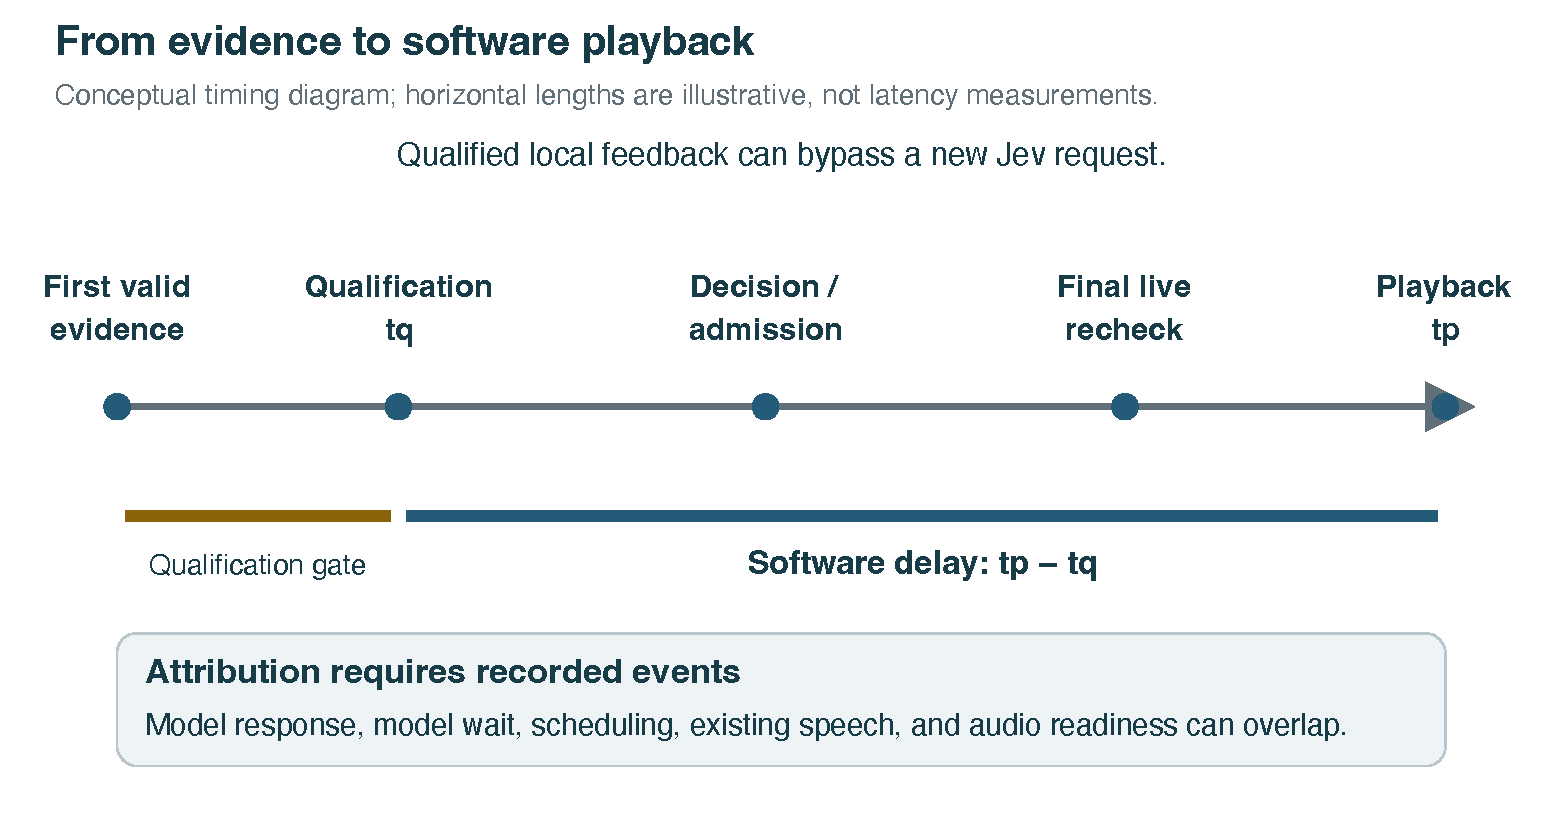
\includegraphics[width=\linewidth,alt={Timeline distinguishes first valid evidence, qualification, admission, final recheck, and software playback; intervals are illustrative.}]{figures/latency-definition.pdf}
\caption[Qualification-to-playback latency and its boundaries]{Conceptual event timeline, not a measured trace. Software delivery delay begins at supported qualification and ends at actual software playback start. The preceding qualification gate and the unmeasured acoustic path are separate quantities. Qualified local feedback can avoid a new cloud request.}
\label{fig:latency-definition}
\end{figure}



Table~\ref{tab:latency-contract} lists the principal timing variables with their endpoints and interpretive limits.
\begin{table}[htbp]
\centering
\caption[Timing variables and evidence boundaries]{Timing contract for planned analysis and engineering evaluation. All cross-clock comparisons require an established mapping; unavailable evidence is not assigned a zero duration.}
\label{tab:latency-contract}
\small
\tagpdfsetup{table/header-rows={1}}
\begin{tabularx}{\linewidth}{@{}p{0.23\linewidth}p{0.31\linewidth}X@{}}
\toprule
Quantity & Endpoints & Interpretation limit \\\midrule
Active completion & Reveal to correct trigger, less union of pauses & Excludes readiness and opening cue; unfinished trials remain unfinished. \\
First gaze contact & Reveal to first valid target-ray hit on active clock & Intersection, not fixation or vicinity acknowledgment. \\
First pointing contact & Reveal to first tracked right-ray hit on active clock & Not the one-second hold or trigger selection. \\
Jev response latency & Request dispatch to response receipt & A response can be deferred, canceled, or stale. \\
Confirmation delivery & Qualified evidence to matching actual software playback & Separate gaze and pointing episodes; not acoustic latency. \\
Live transfer lag & Source event to viewer receipt, if clocks are mapped & Describes transport, not headset decision delay. \\\bottomrule
\end{tabularx}
\end{table}

\subsection{Questionnaire Joins and Versioning}
Final questionnaire administration is separate from the block to which a response refers. A response collected after both blocks retains both its final-administration timing and a Block 1 or Block 2 reference, and the actual voice identifier must be joined through the saved order rather than inferred from block number. Practice is excluded from measured block outcomes even though it uses the first voice.

A convenience export may repeat a block-level workload score on every trial row, but this repetition does not create 40 independent workload observations. The analytical dataset identifies participant-by-block scope and collapses duplicate joins when estimating questionnaire effects. Raw responses, score direction, scale bounds, item identifiers, instrument version, and missingness remain available.

The current NASA-TLX adaptation uses 0--10 ratings, whereas older development exports used 0--100, so automatic scoring must require explicit range metadata. A separately named normalized score can support comparison, but raw values must remain unchanged, and legacy responses whose performance anchors are unknown cannot be scored by guessing their direction. Complete-subscale scoring for IMI and agent-perception measures requires verification before confirmatory analysis.


\section{Planned Statistical Analysis}
\label{ch:analysis}
The analysis asks whether the two voice configurations differ in efficiency and experience. Active completion time is the primary outcome, workload and motivation are secondary, and agent experience, reliance, and debrief responses are exploratory. Because each participant experiences both voices, these outcomes are compared within participants, while guidance diagnostics describe exposure and technical context. Jev and gaze contingency are shared by both conditions, so the statistical comparison concerns voice configuration rather than the independent value of those components.

\subsection{Primary Contrast}
The primary estimand compares active completion time under the self-similar and neutral voices, standardized to the same starting-difficulty distribution. A trial-level mixed-effects analysis of log completion time accounts for participant clustering, voice condition, period/order, trial progression and absolute pre-cue starting theta. The analysis reports the voice time ratio and uncertainty using a two-sided contrast.

Nonlinearity in starting difficulty is represented by a prespecified low-complexity function of theta, while nominal-angle strata support balance plots and a categorical sensitivity analysis. Zero-degree trials remain in the analysis, and completion time is not divided by angle. Before confirmatory recruitment, simulation is used to finalize the model's random-effects structure, angle function and smallest meaningful effect. The participant count requires justification under that same model rather than by treating repeated trials as independent participants.

Figure~\ref{fig:analysis-units} illustrates the planned units of observation. Trial-level measurements are nested within participants, while retrospective ratings remain participant-by-block observations.

\begin{figure}[htbp]
\centering
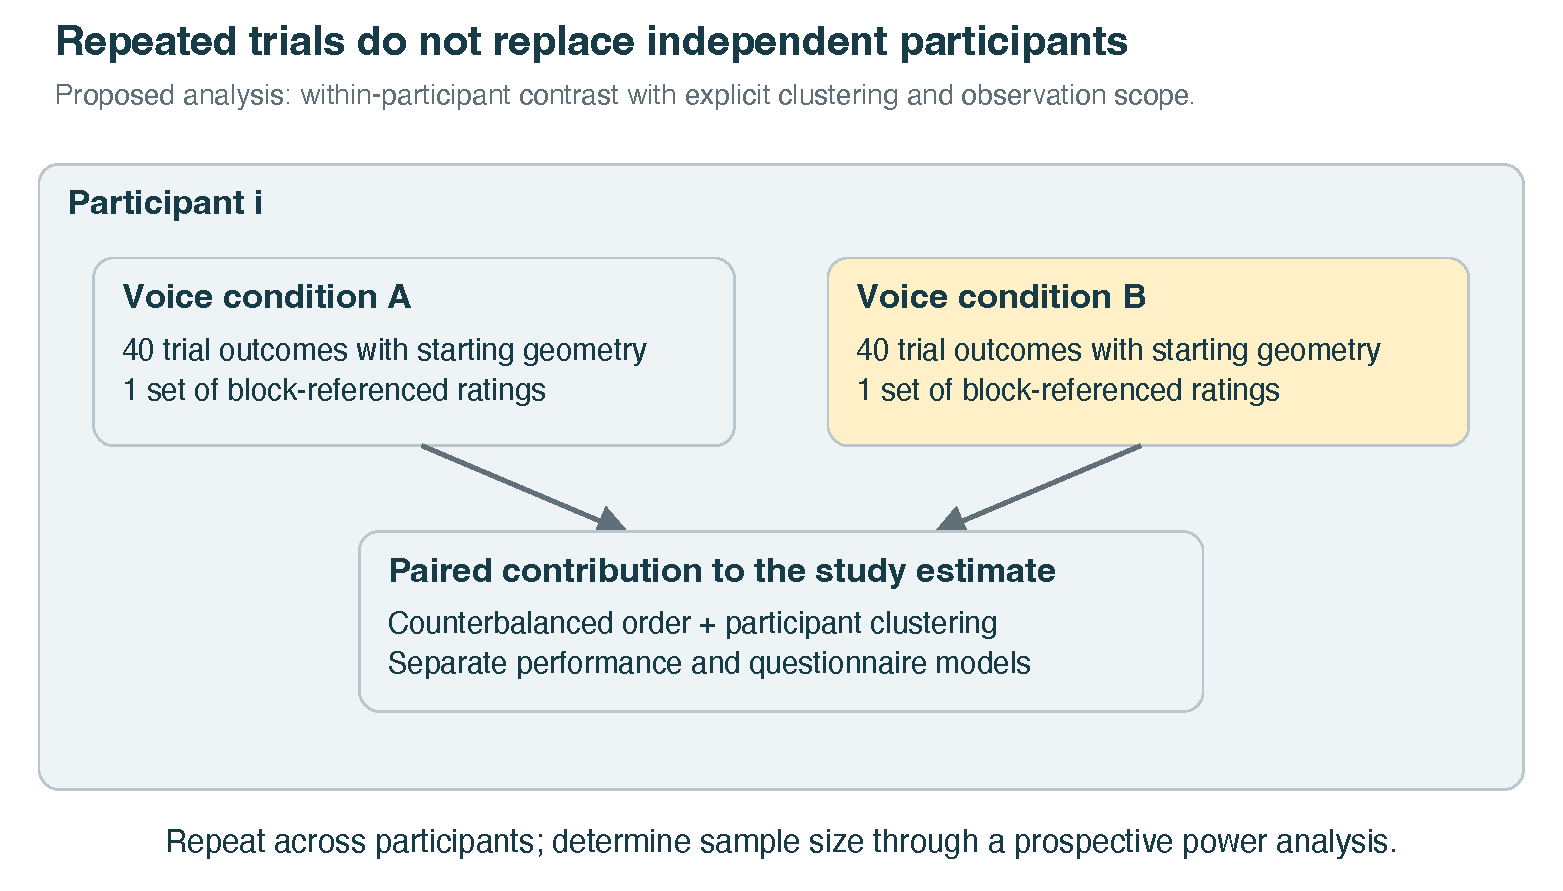
\includegraphics[width=\linewidth,alt={Participant contains two voice conditions, each with 40 trial outcomes and one retrospective questionnaire set, feeding a paired study contrast.}]{figures/analysis-units.pdf}
\caption[Trial nesting and questionnaire analysis units]{Proposed analysis scope. Each participant contributes repeated trial outcomes and two block-referenced questionnaire sets. Counterbalanced order and participant clustering remain part of the analysis plan; additional trials do not replace a justified participant sample size.}
\label{fig:analysis-units}
\end{figure}

Table~\ref{tab:analysis-scope} summarizes the proposed outcome hierarchy and units of analysis. Final contrasts, missing-data handling, and multiplicity families remain to be specified in the preregistration.
\begin{table}[htbp]
\centering
\caption[Planned outcomes and analysis units]{Outcome hierarchy and observation scope. Engineering metrics diagnose the guidance system and do not replace participant outcomes.}
\label{tab:analysis-scope}
\small
\tagpdfsetup{table/header-rows={1}}
\begin{tabularx}{\linewidth}{@{}p{0.20\linewidth}p{0.25\linewidth}X@{}}
\toprule
Role & Unit & Planned interpretation \\\midrule
Primary performance & Trial within participant & Voice contrast in active time, adjusted for starting geometry and design factors. \\
Secondary experience & Participant by referenced block & Workload and separate IMI subscales, retaining paired scope. \\
Exploratory perception & Participant by referenced block & Agent constructs, individual custom items, and voice-similarity manipulation check. \\
Safety & Participant over full session & Recorded discomfort reports, pauses, stops and incomplete exposure. \\
Engineering quality & Qualified event episode / request & Delivery delays, errors, repetition, and provider reliability with distinct denominators. \\
Qualitative experience & Participant response / coded excerpt & Debrief themes with an audit trail, not causal performance estimates. \\\bottomrule
\end{tabularx}
\end{table}

\subsection{A Candidate Primary Model}
A candidate model makes the intended estimand explicit while leaving the final specification to preregistration. For participant $i$, period $b$, and trial $j$, let $Y_{ibj}=\log T_{ibj}$ for successfully completed active-search intervals. A starting specification is
\begin{align}
Y_{ibj}={}&\beta_0+\beta_V V_{ib}+\beta_B B_b+\beta_O O_i\\
&+f(|\theta_{0,ibj}|)+g(j)+u_{0i}+u_{Vi}V_{ib}+\epsilon_{ibj}.
\end{align}
Here $V$ indicates self-similar rather than neutral voice, $B$ identifies the second period, and $O$ identifies assigned voice order. The functions $f$ and $g$ represent prespecified low-complexity effects of exact starting angle and trial progression. In this candidate specification, $j$ indexes position within a block (1--40); the period term represents the between-block change. The exact pre-cue angle depends on the snapshot described in Section~\ref{ch:measurement}, which has not yet been implemented; until it is, the model cannot be fitted as specified, and nominal wall angles must not be relabeled as exact measurements to fill that gap. Participant intercepts and, if supported by the design and model stability, participant voice slopes represent clustering and variation in within-participant contrasts. With only one block per voice, the slope variation can also absorb block-specific session effects; it is not a pure measure of stable individual voice responsiveness. The final random-effects structure remains open; its selection depends on the experimental design and simulation rather than statistical significance~\cite{barr2013random}.

Under this model, the exponentiated voice coefficient, $\exp(\beta_V)$, is a conditional multiplicative time contrast and does not automatically equal a marginal arithmetic mean ratio. The primary estimand therefore remains the marginal contrast standardized over the prespecified common starting-difficulty distribution; the conditional coefficient is reported separately as a model parameter rather than substituted for that estimand. Predictions on the original seconds scale require an explicit retransformation procedure and uncertainty estimate.

A two-period design supports adjustment for period and sequence, but cannot identify every possible asymmetric carryover mechanism independently. For example, using a voice during practice could affect familiarity in its first block, and the second block could benefit from task learning. Period and order terms therefore address these influences only partially, and the report describes residual carryover as a limitation.

\subsection{Sample Size and Precision Planning}
Forty trials per block increase the information available within each participant, but one participant's 80 trials remain correlated observations rather than a substitute for additional participants. A power analysis must reflect the planned trial-level model, between-participant heterogeneity, within-participant correlation, geometry distribution, incomplete trials, and the effect size worth detecting.

The proposed simulation workflow generates participants with both voice blocks and the intended nominal-angle quotas, varying plausible residual variation, participant intercept variation, voice-slope variation, and missingness. Each simulated dataset is fitted with the same model intended for the final analysis, and convergence, bias, interval coverage, and power or precision are summarized across candidate enrollment sizes. The chosen smallest meaningful time ratio and its supporting assumptions require documentation before recruitment. Synthetic pilot values used to test the workflow are labeled as such and are not presented as empirical variance estimates.

A retained pilot can inform variance assumptions only under a documented rule about whether those observations enter the confirmatory sample. The study preserves a build and protocol identifier so that a pilot collected under a different guidance policy can be separated from the frozen release.

\subsection{Secondary Outcomes and Multiplicity}
Condition-specific ratings are collected retrospectively, only after both blocks, with actual survey timestamps retained; each rating set nevertheless remains referenced to a participant-by-block observation. Because these are not immediate post-block measurements, recall and recency effects are considered when interpreting condition differences. Individual workload dimensions and complete unweighted workload means are summarized by participant and block. IMI subscales and the three six-item agent-perception constructs remain separate scores, and the additional Guo Q20--22 appealing, eerie and familiar ratings are analyzed individually rather than combined into an eeriness score. Voice similarity serves as a manipulation check, while custom experience ratings and self-reported guidance use are also analyzed individually.

The analysis retains paired observations and accounts for period where appropriate. The choice between ordinal-item and approximately continuous scale models requires a justification for each measure before confirmatory analysis.

Multiplicity families, secondary contrasts, and adjustment rules require specification before confirmatory analysis. Holm's procedure is available for a prespecified family of confirmatory secondary comparisons~\cite{holm1979simple}; it is not a substitute for deciding which outcomes belong in that family. Exploratory agent-perception and custom-item results are labeled, with effect estimates and uncertainty rather than an indiscriminate list of significance claims.

A participant who does not recognize the clone provides information about the strength of the manipulation and is not excluded solely on that basis; similarly, low liking of either voice is an outcome rather than grounds for exclusion. Sensitivity analyses may examine synthesis quality or recognition, but conditioning on experience that follows assignment changes the interpretation of the contrast, and that change is stated.

\subsection{Data Screening and Missingness}
Data screening first establishes structural integrity: unique participant/session/block/trial keys, consistent voice assignments, chronological reveal and selection events, and required geometry provenance. It then assesses observation coverage and protocol deviations.

A trial with sparse gaze coverage may have valid selection timing yet unreliable gaze-contact latency, so exclusion should be measure-specific where justified. A missing gaze contact does not automatically invalidate completion time, and a complete motion stream does not repair missing voice playback events. Each analysis reports its own denominator and reasons for missingness.

Stopping, timeout, withdrawal, and technical failure require a prespecified treatment. A complete-case time model estimates completion times among observed successful trials under its assumptions, and it may not describe all assigned trials if incomplete outcomes differ by voice. The final plan must therefore also define a complementary completion-probability or time-to-event analysis for use if incompletion is consequential. The revised protocol fixes the active-search deadline at 25 seconds. Deadline-expired attempts are unsuccessful outcomes for completion probability and right-censored at 25 active seconds for a time-to-event analysis; they are not successful 25-second completion times. Earlier development recordings predate this rule and retain their original exposure.

Raw attempts, incorrect selections, pause intervals, timeouts, technical failures and withdrawals are all retained, and stopped trials are not coded as successful completion times. The deadline outcome is recorded separately from technical failure and withdrawal. The remaining treatment of those interruptions and the missing-data estimand require specification before collection; slow successful trials within the deadline are not removed solely for being slow. Missing responses are not replaced with zero; questionnaire scores follow the complete-subscale rule, with item-level missingness reported.

\subsection{Behavior as Outcome Rather Than Automatic Adjustment}
Instruction count, gaze path, and controller behavior can be consequences of voice condition. Including them automatically as primary-model covariates could remove part of the effect the study intends to estimate. The primary comparison therefore adjusts for pre-cue difficulty and design variables. Voice-by-theta variation, selected neutral voice, acoustic quality, guidance timing, and search behavior enter exploratory or sensitivity analyses with their assumptions reported.

For example, slower search can produce more opportunities for guidance, and more guidance can itself affect search time. A correlation between instruction count and duration does not establish that speech caused delay.

\subsection{Guidance Delivery Evaluation}
Engineering analysis distinguishes event qualification, decision latency, model deferral, scheduling delay and actual playback, and it evaluates gaze and controller confirmation separately. Sequence-level review includes what happened before and after each cue. Automatic checks and ratings produced by an offline language-model evaluator (Appendix~\ref{app:scenarios}) remain advisory engineering evidence rather than participant perception scores.

\subsection{Additional Performance and Eye-Behavior Figures}
Missed-target percentages complement completion-time distributions, with the number of completed, timed-out, technically interrupted, and unresolved attempts shown explicitly. For the participant study, paired participant summaries by voice condition are preferable to treating all trial rows as independent observations. Earlier unconstrained development recordings are kept separate from searches governed by the new deadline.

After independent detector validation, possible additional figures include fixation-count distributions, saccade rates with their valid-time denominators, and IPA distributions with retained pupil coverage, each separated by voice condition and participant. Last-target-fixation duration requires validated events and a target-area join. No EEG or ERP plot can be generated from the current headset logs. Until those requirements are met, the candidate-eye figures in Section~\ref{sec:development-eye-candidates} serve only to inspect the processing pipeline; they do not test a voice effect or infer workload. Threshold sensitivity and missing-data summaries accompany each derived outcome.

\subsection{Qualitative Analysis and Mixed Evidence}
The debrief begins with broad experience questions, followed by balanced probes about voice preference, perceived performance, comfort, and potential uses. The coding process records the initial codebook, revisions, coding decisions, and independent review of a subset. Contradictory or minority accounts are retained rather than forced into one favorable theme.

Reported reliance and observed behavior are considered together without treating either as a perfect measure of the other. The final report separates quotations, coder interpretation, and behavioral evidence.

\subsection{Safety Outcomes and Manipulation Checks}
Safety reporting describes recorded discomfort reports, pauses, stops and incomplete exposure, including the reason for each interruption when available. These observations document tolerability and session completion; they do not provide a standardized pre-to-post symptom score. The operational stopping procedure must be frozen before participant collection.

The similarity manipulation check reports the paired difference between self-similar and neutral-voice ratings with uncertainty. A group-level decision rule and any practically meaningful difference remain open preregistration decisions. Because equivalence testing is not currently specified, a nonsignificant voice contrast is not interpreted as equivalence.

\chapter{RESULTS}
\label{ch:evaluation}
The results chapter returns to the question posed in the introduction: does guidance spoken in a synthetic version of the participant's own voice differ, in efficiency or experience, from guidance spoken in the neutral voice the participant selected? The chapter first establishes how the comparison is delivered, then addresses search efficiency, workload, motivation, and exploratory measures of voice experience. Because confirmatory participant data have not yet been collected, the sections below describe the reporting structure for each result and separate those pending results from the development evidence available for the apparatus.

\section{Recorded Development Results}
\label{sec:development-results}
The following descriptive results come from actual headset recordings, rather than simulated trials. The analysis includes all nine locally mirrored \texttt{DEV\_NEUTRAL} recordings dated October 19--20, 2026 (Runs 20--28), with 27 started searches and 21 recorded correct selections. These sessions used the neutral-male development mode; the eight available trial summaries identify the Eric voice and a 168-object layout. This is an earlier development configuration, not the frozen participant-study stimulus configuration. Each recording identifies a different build, and the shared development label does not establish a sample of independent participants. The results therefore describe operation during testing, not a self-similar versus neutral voice effect or a controlled comparison between software versions.

The analysis retains unfinished searches and uses the complete recorded prefix of Run 21, whose final JSON record is truncated. No missing endpoint is reconstructed. Source file hashes, recording identifiers, derived CSV tables, and the plotting script accompany the thesis sources under \texttt{development-results/}. Twenty of the 21 completed-search durations also match the separately saved trial summaries within their 0.01-second rounding precision; Run 21 has no corresponding summary in the inspected mirror. This comparison checks agreement between exports, not independent timing accuracy.

\subsection{Search Completion During Development}
Figure~\ref{fig:development-search} separates completed-search durations from recording coverage. Panel~(a) shows each completed search, with box plots for runs containing at least three completions; runs with fewer completions show individual observations only. Runs with no recorded completion remain labeled with zero observations. Panel~(b) includes all 27 started searches and identifies the six unfinished searches. These unfinished endpoints are not completion times or evidence of task failure: a recording may end while the user is testing, pausing, or leaving the application. The logarithmic duration axis retains the longest completed search while allowing shorter searches to remain distinguishable.

The figures use compact, labeled panels and distribution summaries, following the presentation of descriptive results in Chiossi et al.~\cite{chiossi2024searching}. Boxes span the first and third quartiles, the central line marks the median, and whiskers extend to the most extreme observations within 1.5 interquartile ranges. Every observation remains visible as a point, including values beyond the whiskers. Horizontal offsets separate points for legibility and do not alter measured values. Colors distinguish adjacent runs for readability and do not represent experimental voice conditions. No confidence intervals or significance annotations are estimated from these development recordings.

Among the 21 completed searches, the median recorded active-search duration is 19.56~s, the 95th percentile is 44.43~s, and the maximum is 275.92~s. Percentiles use linear interpolation between ordered observations. The long completed search is retained rather than removed as an outlier: these were unconstrained development sessions, and the logs do not establish that every active second represents uninterrupted task-directed effort. The plotted counter excludes time according to the application's search-timer logic and should not be confused with elapsed recording time. The distribution establishes that the application records completed selections and variable search durations; it does not estimate participant efficiency under a standardized protocol.

\begin{figure}[htbp]
\centering
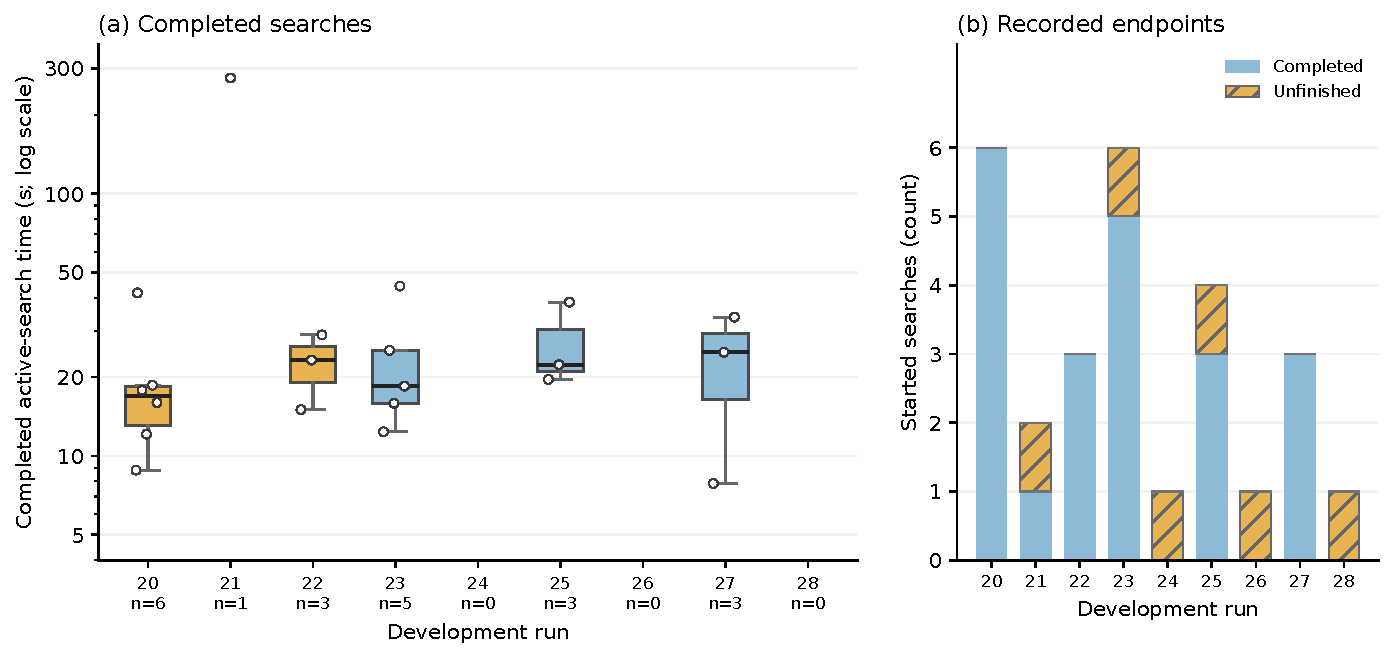
\includegraphics[width=\linewidth,alt={Two panels show development Runs 20 through 28: 21 completed search durations as individual points and quartile boxes on a logarithmic seconds axis, and counts of 21 completed and six unfinished searches. Runs without completions are labeled n equals zero.}]{figures/development-search-times.pdf}
\caption[Recorded development search durations]{Recorded development searches. (a) Completed active-search times, with individual observations, sample counts, and quartile boxes where at least three observations are available; the vertical axis is logarithmic. (b) Counts of completed and unfinished searches. Unfinished searches are excluded from duration summaries, not assigned a completion time.}
\label{fig:development-search}
\end{figure}

\subsection{Speech Delivery and Earlier Waiting}
Of 350 software playback-start events during the recorded search intervals, 339 have an unambiguous chronological match to a guidance request, audio request, and audio-ready event using the same recording, trial, and decision identifier. The remaining 11 playback events are excluded from the latency distribution because the required join is missing or ambiguous. They are not assigned zero delay. Requests that never produced playback also do not enter this delivered-event distribution.

For the 339 matched events, the median interval from the delivered decision's request to software playback is 0.244~s, with a 95th percentile of 0.487~s and a maximum of 0.538~s (Figure~\ref{fig:development-speech}). The median request-to-audio-request interval is 215.7~ms, compared with 17.9~ms from audio request to readiness and 1.0~ms from readiness to playback. The first interval can include decision-making and scheduling; it is not an isolated measurement of Jev network latency. These timestamps measure software events, not the onset of audible sound at the headset.

\begin{figure}[htbp]
\centering
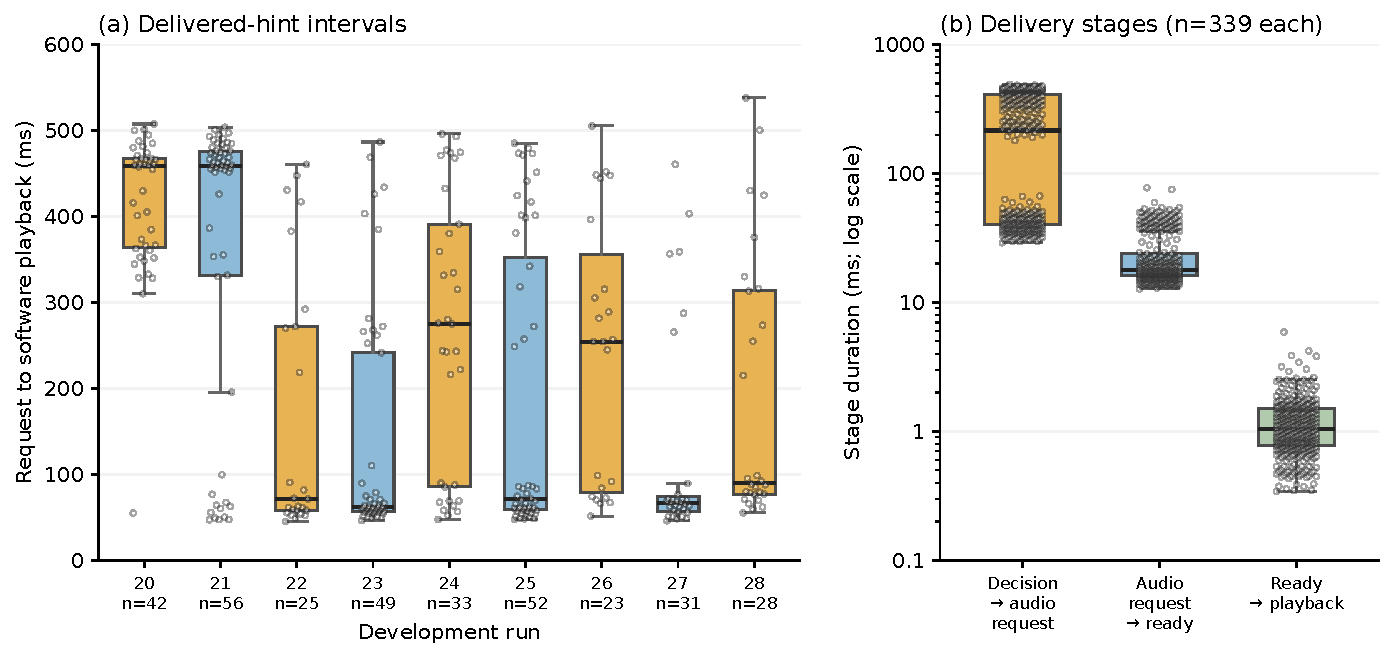
\includegraphics[width=\linewidth,alt={Two panels show 339 matched delivered hints: request-to-playback distributions by development run on a linear milliseconds axis, and the three recorded delivery-stage distributions on a logarithmic milliseconds axis. Each panel shows individual recorded events and quartile boxes.}]{figures/development-speech-delivery.pdf}
\caption[Software speech-delivery intervals]{Software speech-delivery intervals for 339 matched playback events. (a) Request-to-playback distributions by run, with sample counts. (b) Delivery-stage distributions for the same events, using a logarithmic vertical axis. Points retain all observations; boxes and whiskers follow Figure~\ref{fig:development-search}. Earlier qualification and deferral, undelivered requests, and acoustic onset are outside this measure.}
\label{fig:development-speech}
\end{figure}

Short delivery intervals do not establish prompt feedback from the user's perspective. Figure~\ref{fig:development-confirmation} reconstructs the previously investigated gaze-confirmation episode in Run 20, Trial 4. A gaze-qualified hint request is recorded at session time 321.426~s. Three successive transmission snapshots record qualified target gaze, while controller-hold qualification is false. Jev returns \emph{wait}, \emph{wait}, and then \emph{speak}; playback of ``You've got it!'' begins at 323.616~s. The interval from the first qualified request to playback is therefore 2.190~s, although the final request-to-playback interval is only about 0.352~s. This is one delayed episode with repeated requests, not three independent confirmation failures. The snapshots document qualification at those instants; they do not independently establish uninterrupted fixation between them.

\begin{figure}[htbp]
\centering
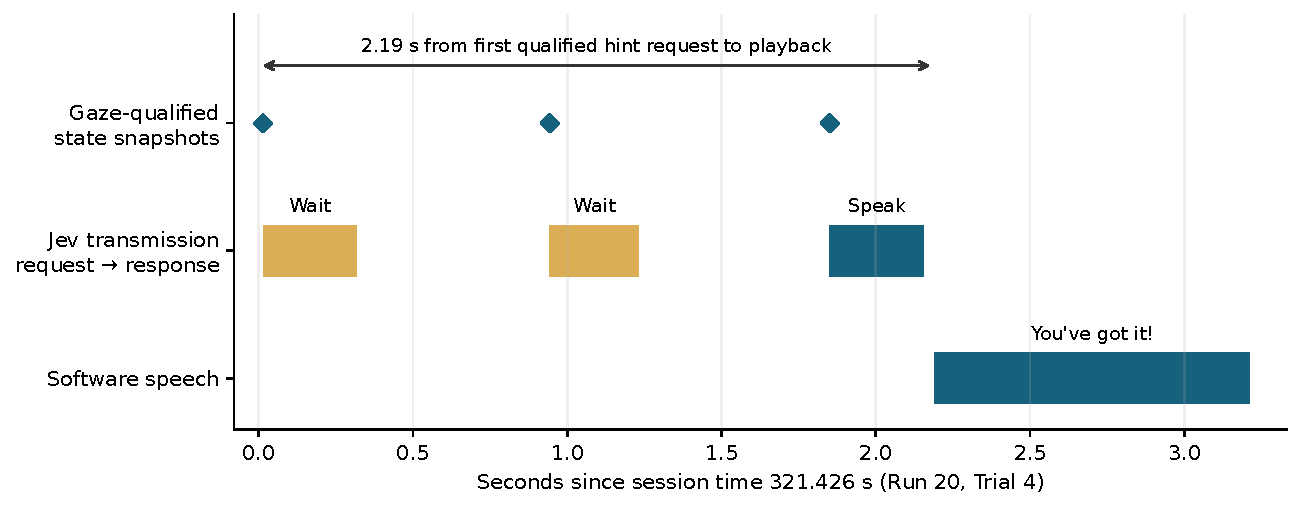
\includegraphics[width=\linewidth,alt={Run 20 Trial 4 timeline: three gaze-qualified snapshots accompany two wait decisions and a speak decision. The confirmation begins 2.19 seconds after the first qualified request. Controller hold is unqualified at all three snapshots.}]{figures/development-confirmation-sequence.pdf}
\caption[Recorded gaze-confirmation delay]{Recorded gaze-confirmation delay in Run 20, Trial 4. Diamonds mark qualified-state snapshots, bars mark transmission request/response intervals and software speech. Gaze confirmation is distinct from controller confirmation and correct trigger selection.}
\label{fig:development-confirmation}
\end{figure}

This case demonstrates why sequence history is required alongside aggregate delivery statistics. Earlier waiting remains visible even when the request that ultimately produces speech is processed quickly. The historical recording does not establish whether subsequent changes eliminated this behavior; that question requires a comparable recording from the revised build. No acoustic-latency or participant-perception conclusion is drawn from this trace.

\subsection{Recorded Gaze Usability}
Figure~\ref{fig:development-gaze} summarizes 58,041 rendered-frame replay samples recorded during active search. A sample is counted as usable when the saved gaze-device availability flag is true and the replay's gaze-usable flag is set. This is the application's recorded usability decision, which includes tracking and freshness checks, rather than a new physiological classification. Samples marked unusable are retained, and absent or indeterminate flags would be classified as unknown.

Across the nine runs, usable-row fractions range from 63.75\% to 99.97\%. All inspected active-search rows have a usable/unusable classification; however, intervals with no recorded rows remain unobserved and are not included in the denominator. The dominant logged invalidity reason is \texttt{both\_native\_eyes\_invalid}. That diagnostic does not by itself distinguish blinking, headset removal, poor fit, calibration, or a software issue. Runs with long periods of unusable gaze warrant timeline inspection before they are used to assess guidance behavior.

\begin{figure}[htbp]
\centering
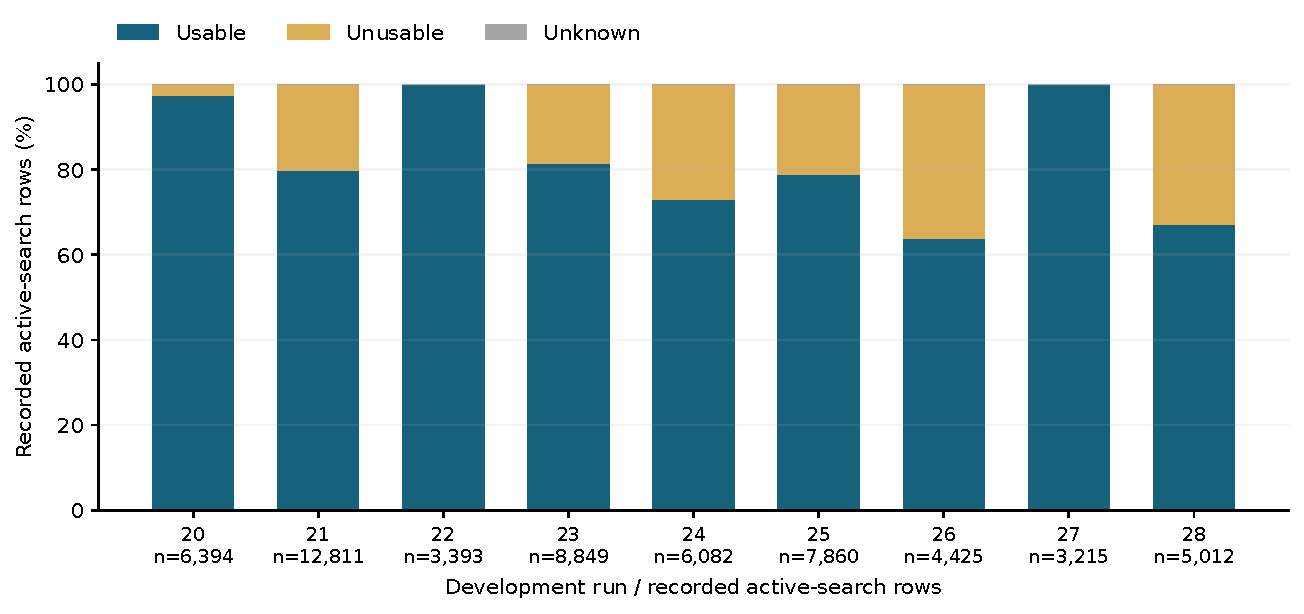
\includegraphics[width=\linewidth,alt={Stacked bars show usable and unusable active-search replay rows for development Runs 20 through 28, with denominators below each bar. Usable fractions range from 63.75 to 99.97 percent; no inspected row has an unknown flag.}]{figures/development-gaze-usability.pdf}
\caption[Recorded gaze usability during development]{Recorded gaze usability during active search, with the number of replay rows shown for each run. These are rendered-frame observations, not independent native sensor samples. Unrecorded intervals are outside the denominator.}
\label{fig:development-gaze}
\end{figure}

The row fractions are not estimates of spatial accuracy, native acquisition frequency, fixation quality, or the proportion of total search time with valid gaze. Their role is diagnostic: they identify differences in the evidence available to the guidance system during these development recordings. Together, the search, delivery, and usability plots document the apparatus before the planned voice comparison, while leaving performance and experience differences between voices unresolved.

\subsection{Exploratory Eye-Measurement Pipeline}
\label{sec:development-eye-candidates}
A separate analysis uses the recorded eye-observation file for development Run 30 (October 23, 2026), which contains five recorded search identifiers in neutral-male mode. These searches precede the new deadline configuration; their retained durations are not truncated to 25 seconds. Figure~\ref{fig:development-eye-candidates} presents per-eye candidate fixation counts, candidate saccade rates, exploratory IPA, and pupil duration retained for IPA. The figure uses only measured records; artificial test signals used to verify the code are excluded.

The strict pupil screens retain approximately 2.18, 2.25, 4.22, and 5.28 seconds per eye for the first four searches, with no accepted segment for the fifth. These short retained windows are not estimates of whole-trial workload, and an unavailable IPA value is not a zero. Separate left- and right-eye values expose disagreement rather than averaging it away. The candidate fixation counts and restricted saccade rates likewise depend on detection thresholds and on the available query-time evidence. Three illustrative parameter variants are exported for sensitivity inspection, without choosing a setting on the basis of a favorable result.

\begin{figure}[htbp]
\centering
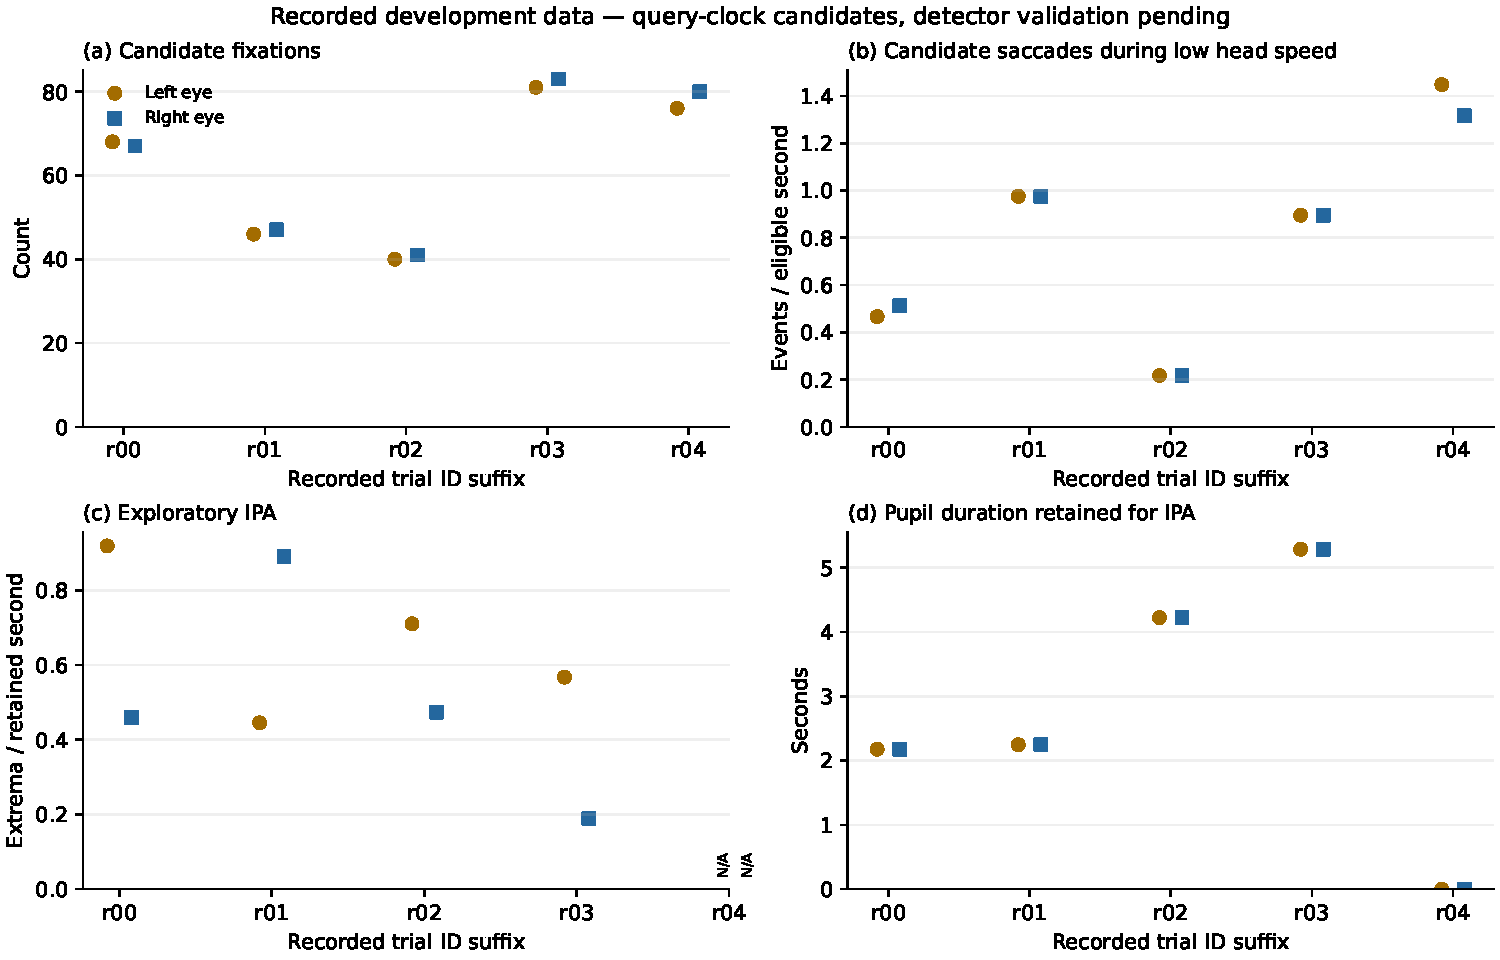
\includegraphics[width=\linewidth,alt={Four panels show actual Run 30 per-eye candidate fixation counts, saccade rates during low head speed, exploratory IPA and retained pupil duration for five searches. The fifth search has unavailable IPA. All eye-event classifications remain unvalidated.}]{figures/development-eye-candidates.pdf}
\caption[Exploratory eye-measurement output from recorded data]{Run 30 development diagnostics. (a) Candidate fixation counts. (b) Candidate saccade events per retained low-head-speed second. (c) Exploratory IPA extrema per retained pupil second. (d) Retained pupil duration. Points represent separate eyes within recorded searches, not independent participants. The software-query clock does not establish 120-Hz sensor acquisition, and the classifications require independent validation.}
\label{fig:development-eye-candidates}
\end{figure}

The source hash, detector configuration, dependency versions, individual event intervals, summary CSV, and threshold-sensitivity table are retained with the thesis development artifacts. Computational checks pass, but no independently labeled headset sequence is yet available to establish event precision, recall, or duration error. These results demonstrate an executable measurement workflow and identify data limitations; they do not supply participant-study findings.

\subsection{Outcome Panels by Voice Condition}
\label{sec:development-voice-panels}
Figure~\ref{fig:development-voice-panels} adapts the four-panel presentation of accuracy, missed targets, search time, and pupil activity in Chiossi et al.~\cite{chiossi2024searching} to the present study's voice conditions. Each horizontal axis distinguishes \emph{Neutral voice} from \emph{Self-similar voice}; AR/VR and physical/virtual subdivisions are not factors in this comparison. The current observations come from development Run 30. Its five started searches all use the neutral voice, so the self-similar position remains explicitly unpopulated. Scheduled searches that never started do not contribute observations.

First-selection accuracy is 80\%: four of the five completed searches contain no incorrect trigger selection before the correct selection. This is a run-level proportion among completed searches, rather than a distribution across participants or a measure of success before the new deadline. Active-search completion times use the recorded search counter and retain their original values in seconds. Run 30 has no recorded 25-second deadline, so its missed-target percentage is unavailable; searches lasting longer than 25 seconds are not retrospectively classified as misses.

For the condition-level display, exploratory IPA is the arithmetic mean of the available left- and right-eye candidate rates within each search. Four searches have values from both eyes; the fifth has no eligible pupil segment and remains missing. This display summary is not a validated workload score, and the separate-eye diagnostics and retained durations remain available in Figure~\ref{fig:development-eye-candidates}. Points in the time and IPA panels denote repeated trials within one development run. They do not represent independent participants, and the figure supports no estimate of a voice-condition effect. The participant-study comparison requires observations from both voices and paired participant summaries using consistent scoring and eligibility rules.

\begin{figure}[htbp]
\centering
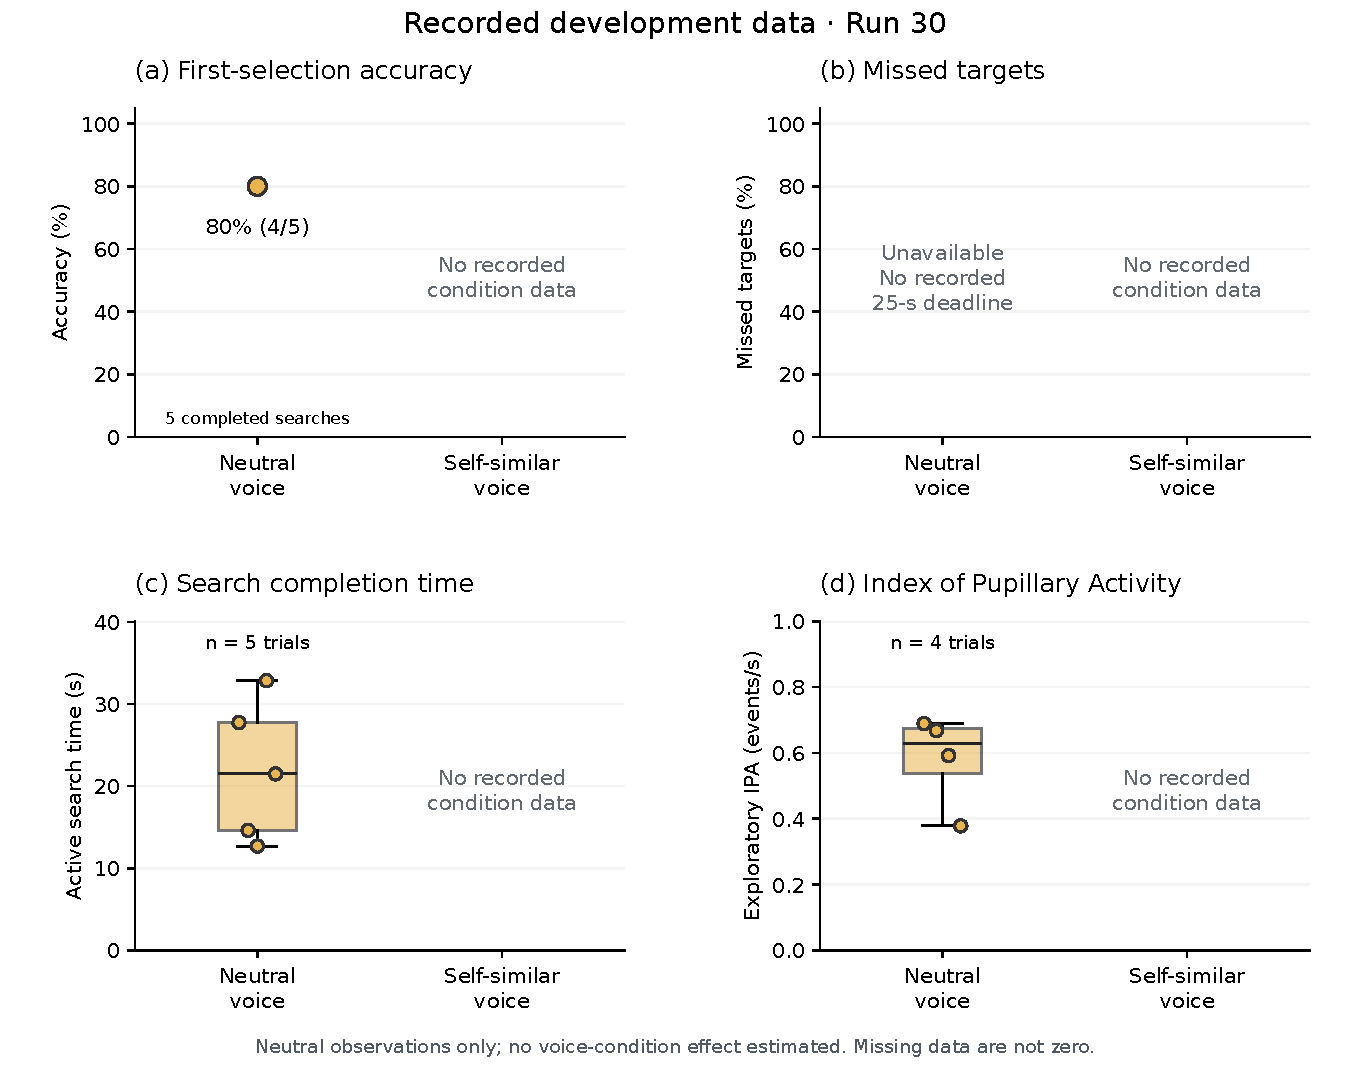
\includegraphics[width=\linewidth,alt={Four development outcome panels use Neutral voice and Self-similar voice on every horizontal axis. Neutral Run 30 has 80 percent first-selection accuracy among five completed searches, five active search times, and four exploratory IPA trial means. Missed-target percentage is unavailable without a recorded deadline. Self-similar data are absent in every panel.}]{figures/development-voice-condition-panels.pdf}
\caption[Development outcome panels by voice condition]{Development outcome panels arranged for the neutral versus self-similar voice comparison. (a) First-selection accuracy among completed searches, shown as one run-level point. (b) Missed targets, unavailable for this recording without a recorded deadline. (c) Active search completion time. (d) Exploratory IPA averaged across available eyes within each trial. Boxes in (c) and (d) show quartiles and median, with 1.5-IQR whiskers; all observed trial values are shown. Unavailable values are not plotted as zero. No self-similar observations or inferential comparisons are included.}
\label{fig:development-voice-panels}
\end{figure}


\section{Planned Reporting of Participant Results}
Participant reporting begins with participant flow, exclusions, incomplete sessions, and data coverage by condition and order. It then describes realized starting geometry and the similarity manipulation check before presenting the primary voice contrast.

The primary result includes the fitted time contrast, its uncertainty, the analyzed participant and trial counts, and model diagnostics. Secondary reporting covers workload and IMI subscales at participant-by-block level, followed by exploratory sections on agent perception, voice experience, guidance behavior, and debrief themes. Each table states its denominator and identifies missing observations.

\begin{table}[htbp]
\centering\caption{Planned result families and their status. No confirmatory participant outcomes are reported here.}
\small\tagpdfsetup{table/header-rows={1}}
\begin{tabularx}{\linewidth}{@{}p{0.27\linewidth}XX@{}}\toprule
Result family & Required evidence & Present status \\\midrule
Participant flow & Consented, started, completed, stopped; reasons & Not available \\
Manipulation check & Similarity by voice with paired scope & Not available \\
Primary performance & Adjusted time contrast and uncertainty & Not estimated \\
Workload and IMI & Versioned raw items and complete subscales & Not collected for this report \\
Agent experience & Individual and construct-specific ratings & Not collected for this report \\
Guidance quality & Sequence-level playback and evidence & Development traces reported; study comparison pending \\
Debrief themes & Recorded responses and coding audit & Not available \\\bottomrule
\end{tabularx}
\end{table}


\subsection{Results Organized by Research Question}
Following the manipulation check, the reporting framework addresses each research question in turn. For the primary question, the estimand is the marginal time contrast standardized over a common starting-difficulty distribution, as defined in Section~\ref{ch:analysis}; here, \emph{standardized} refers to that common distribution rather than to a standardized effect size. The estimate is accompanied by its uncertainty, the eligible participant and trial counts, and model diagnostics, following the analysis plan finalized before confirmatory recruitment. Secondary reporting covers the paired workload outcomes and the separate IMI subscales, using multiplicity families to be defined in the analysis plan. Exploratory reporting presents agent-perception and custom ratings alongside debrief themes and valid search measures. A contrast that cannot be estimated or proves inconclusive is reported as such rather than omitted.

Guidance delivery is reported separately through sequence coverage, qualification-to-playback delay, provider reliability, and categorized faults. Software tests and language-model ratings characterize the apparatus, not its effects on participants; conversely, a voice-condition difference does not show that every instruction was delivered correctly.

\section{User Performance}
Once participant data are collected, this section will report active search-completion time, incorrect trigger selections, and valid gaze/controller contact latencies by voice condition. Reporting includes paired participant summaries and the planned adjusted contrast, with sample counts and uncertainty.

\section{User Experience}
Once participant ratings are collected, this section will report condition-referenced workload, the separate motivation subscales, agent experience, voice liking and similarity, and debrief responses. No questionnaire responses or preference distributions are simulated.

\section{Apparatus Verification}
In addition to the development recordings in Section~\ref{sec:development-results}, software verification records document the apparatus. A verification run on October 20, 2026 passed schedule and voice-isolation checks confirming one practice trial in the first assigned voice, two measured blocks, and the nominal-angle quotas; it also passed 38 trial-export tests and seven workload scoring and plotting tests, and the Android application was built, installed, and launched successfully. These test counts come from that run and were not re-executed for this manuscript. The current software version, dated October 25, 2026, includes the pre-cue snapshot and balanced direction and height allocation. Its schedule checks pass across 50 participant identifiers and both voice orders, and its geometry checks pass across every starting wall and angle category.
\begin{table}[htbp]
\centering\caption{Apparatus verification and outstanding validation.}
\small\tagpdfsetup{table/header-rows={1}}
\begin{tabularx}{\linewidth}{@{}p{0.28\linewidth}XX@{}}\toprule
Component & What was verified & Not yet established \\\midrule
Schedule and voice checks & One practice trial and nominal allocation of 40 trials in each of two blocks pass automated checks & Wearer completion of a full session \\
Trial export and TLX tests & Declared scales and retrospective joins are correct in tested cases & Validation of all questionnaires \\
Unity integration checks & Listed state and interaction cases pass & Robustness to all timing races \\
Android build/install/launch & Application built, installed, and started & Acceptance in a participant session \\
Exact pre-cue theta & Snapshot saved at readiness completion; geometry checks pass & Observation in a complete wearer session \\
Vertical allocation & 20/20 and per-angle height quotas pass schedule checks & Target visibility and seated comfort \\
Voice-condition outcomes & None; no confirmatory dataset reported & Any performance or preference conclusion \\\bottomrule
\end{tabularx}
\end{table}


\section{Guidance Quality Supporting the Voice Contrast}
Reporting describes gaze availability, actual speech exposure, delayed acknowledgments, interruptions, and unhelpful cues by voice condition and session. This account helps assess whether technical delivery problems affected one condition more than the other. The voice contrast is not automatically adjusted for behavior-dependent hint counts or waiting time: these quantities arise after voice assignment, may themselves depend on voice condition, and cannot be treated as baseline difficulty (Section~\ref{ch:analysis}).

Gaze acknowledgment, controller acknowledgment, and correct trigger selection remain separate events. Their sequence records document feedback delivery, whereas participant ratings and debriefing address how that feedback was experienced. Appendix~\ref{app:scenarios} defines sequence tests and evaluation criteria for assessing the apparatus before interpreting differences between voices.

\chapter{DISCUSSION AND LIMITATIONS}
\label{ch:discussion}
\section{What the Study Can Explain}
Follow My Voice asks whether a synthetic voice resembling the listener changes search efficiency or experience relative to a neutral voice the listener has already chosen. Because participant results are pending, each interpretation is stated conditionally, as a reading the data could support rather than a conclusion about which voice is better.

The discussion distinguishes three kinds of evidence. The primary question concerns measured efficiency, the secondary questions concern workload and motivation, and the exploratory questions examine participants' evaluations of the voices and their reported reliance on guidance. Agreement among these outcomes could strengthen a design interpretation, whereas disagreement could reveal a tradeoff that a single outcome would conceal.

\section{Interpreting Efficiency and Experience Together}
If completion time favors the self-similar voice, interpretation considers the estimate's uncertainty together with the manipulation check and guidance quality. A difference accompanied by systematic intelligibility or delivery problems in the neutral condition could reflect those problems rather than anything specific to self-similarity. If both conditions have comparable delivery quality and participants recognize the clone, the result would more directly support a voice-condition effect in this task, although it would still not separate resemblance from other differences between the chosen and synthesized voices.

Faster completion with the neutral voice would be consistent with a chosen external voice being easier to follow, but also with intelligibility or delivery problems in the cloned condition. Delivery records and acoustic-quality reporting could help distinguish these readings, although the study could not establish the mechanism without further evidence. Liking, naturalness, and reliance ratings may help characterize the experience in either case, but a correlation between such ratings and performance would not show that they mediate the voice effect.

If completion times are similar, the width of the uncertainty interval becomes central. A wide interval would leave practically important differences unresolved, whereas a narrow interval near the null could constrain the size of a plausible effect under the tested conditions. A nonsignificant test alone does not establish equivalence. Equivalence testing is not part of the current analysis specification, and adding it would require a meaningful bound and procedure defined before inspecting the result.

A preference for self-similar speech may occur without a detectable improvement in completion time, while efficient search may coexist with discomfort.

Kao et al. examine an avatar voice in a setting where continued voluntary play can reflect engagement, whereas Guo et al. report favorable impressions alongside eeriness in virtual collaboration~\cite{kao2021selfsimilar,guo2024doppelganger}. Here, a voice instructs the listener through a fixed search task. Faster completion therefore addresses efficiency, while enjoyment, discomfort, and debrief responses address the experience of following it.

\section{Practical Relevance and Transfer to Other Search Tasks}
The applications motivating the introduction identify where guided search could be useful, rather than domains already validated by this experiment. Locating task-relevant items in maintenance or training, finding a book, and noticing relevant VR content share a need to connect assistance with something in the environment~\cite{binetti2021outofview,zhang2023seehear,lange2020hivefive}. The present study examines a voice-choice question within that interaction; it does not test industrial task completion, learning transfer, navigation safety, or narrative comprehension.

The practical value of the study depends on how its outcomes combine. Faster search accompanied by acceptable workload and a comfortable voice experience would support considering self-similar guidance for comparable tasks. A favorable experience without a detected speed difference could still motivate offering the clone as an optional voice, though not claiming that it makes search more efficient. Discomfort, intelligibility problems, or a preference for the neutral voice would instead mark limits to that option.

Transfer also depends on how much information users already have. Here, the participant must use spatial guidance to infer an initially unnamed target; in Zhang et al.'s book task, the target title was supplied~\cite{zhang2023seehear}. A known-target task may allow people to continue independently and encounter the voice less often. Real work can additionally require recognizing meaningful parts, remembering procedural steps, moving through space, or coordinating with another person. Replication in those contexts would need to establish both the quality of guidance and the effect of voice choice.

\section{Voice Identity and Acoustic Confounds}
The voice conditions may differ in acoustic properties as well as perceived resemblance. The self-similar voice depends on recording quality and synthesis, whereas the neutral voice comes from a heterogeneous catalog, and the two may differ in pitch, prosody, speaking rate, pronunciation, and clip duration. Because the same words and provider do not guarantee matched acoustics, the study documents these properties and pilot intelligibility at comfortable playback levels rather than claim exact equivalence.

The variety of chosen neutral voices is a deliberate consequence of the design: requiring every participant to hear the same neutral voice would replace the comparison with a preferred alternative by a comparison with a fixed one. The analysis should retain chosen voice identifiers and describe the distribution, while avoiding an overfitted model with unsupported estimates for sparsely chosen voices. An exploratory association between a neutral voice and performance may reflect who selected it as well as its acoustic properties.

The current self-similar manipulation applies no additional pitch shift, panning, or inner-thought treatment. Earlier development attempts to make cloned speech sound like an internal monologue are not part of the study, and reintroducing such an effect in only one condition would change the manipulation and require a revised rationale and analysis.

\section{Adaptive Guidance as a Shared Mechanism}
Gaze-dependent sonification, staged spatial cues, and audiovisual assistance investigate different ways to connect a cue with a search target~\cite{losing2014guiding,kwok2022twostep,binetti2021outofview}. Follow My Voice adapts these precedents into spoken orientation and refinement so that the assigned voice participates throughout the task. A difference between the two voice conditions would not demonstrate that speech outperforms those techniques, or that Jev improves search: neither comparison is part of the participant design.

A shared policy does not produce identical spoken sequences. Because participants turn, pause, look, and point differently, the policy supplies different directions and can emit different numbers of hints.

Nevertheless, policy drift would threaten the comparison. Changing phrases, timers, or provider behavior midway through collection could alter assistance quality. The study release must pin the application build, configuration, phrase semantics, voice preparation settings, and decision-provider version where possible. Any unavoidable service change must be documented and considered in the analysis.

The central state machine improves auditability by assigning guidance evidence and transitions to a single local component, but it cannot guarantee correct guidance. Calibration error can produce an incorrect observation, an unclear reference frame can produce an unhelpful phrase, and a stale response can pass an incomplete check.

\section{Practice, Learning, and Order}
One practice trial reduces setup burden but provides limited exposure to a complex interaction in which a participant must learn to hold gaze on the readiness cross, follow speech, use the chair comfortably, aim the right controller, and press the trigger to select. A fixed single trial does not prove that every participant has acquired these skills equally, and the practice-proficiency rule remains to be established through pilots.

Practice uses the first assigned voice, which aligns initial exposure with the first block but also couples practice familiarity with period. Counterbalancing helps distribute this coupling across voice conditions; it does not prevent fatigue, learning, novelty, or asymmetric carryover. These limitations are reported with period and order effects and any relevant sensitivity analysis.

\section{Retrospective Questionnaires and Burden}
The final-only survey avoids interrupting the two-block search sequence with a long questionnaire, but it also requires participants to recall Block 1 after completing Block 2. Ratings may therefore reflect recency, contrast, or imperfect recall. Each rating set identifies its referenced block; the reminder linking that block to its voice remains to be piloted. These reminders may aid recall but cannot guarantee accurate recollection.

The condition-specific battery contains 130 numeric responses across both blocks, in addition to setup ratings, comparison questions, and debrief. Its completion time, missingness, and comprehension therefore require pilot measurement. Because participants may be tired or uncomfortable after exposure, researchers check whether they are comfortable continuing before administering the retrospective sets.

Adapting an embodied-agent measure to a voice agent can alter its meaning. Co-presence or anthropomorphism items may be understood differently without a visible character. The thesis retains attribution and wording changes, reports the adaptation, and avoids asserting new psychometric validation from a small experimental sample. Custom reliance and naturalness items remain individual exploratory measures.

\section{Gaze Quality and Feedback Coupling}
Gaze serves both as an input to assistance and as a recorded behavioral signal. Tracking gaps can change the participant's experience and reduce measurement coverage, affecting both the outcome being measured and the evidence available to interpret it. Coverage and technical events are considered alongside performance without automatically being treated as pre-existing participant characteristics.

A highlighted vicinity candidate can help indicate what the system currently attends to, but it can also suggest a reference object that differs from the mathematical gaze ray. For example, an instruction to look lower can be consistent with a gaze ray above the target yet confusing if the target appears higher than a highlighted neighbor. A cue should be evaluated in its visible interaction context, not solely against the sign of a geometric delta. Development-only rings and diagnostic markers must not silently enter the participant condition.

The proposed validity-aware stream and independent calibration checks address these risks, but headset-specific spatial performance and the rate of distinct gaze observations remain empirical questions. Validation results for the Vive Pro Eye cannot substitute for Focus Vision measurements, and an interaction threshold chosen for usability does not establish a validated measure of cognition.

\section{Privacy, Consent, and Reproducibility}
Coding participant identifiers does not make voice recordings anonymous, because both natural and synthesized speech can remain recognizable. The consent and data-management documents must describe recording, synthesis, cloud processing, storage, access, and deletion using the services actually employed. Older local-only descriptions are inconsistent with current ElevenLabs voice preparation and Jev decisions and require reconciliation before participant use.

The thesis reports the relevant processing stages without including credentials or identifiable recordings. A reproducibility package can provide code, versioned schemas, example synthetic records, and de-identified summaries where authorized. Distribution of cloned voices or raw participant audio requires a separate basis and must not be assumed from consent to participate.

Cloud dependencies also affect replication. A future researcher may not obtain the same voice model or identical decision behavior. Preserving prepared-library metadata and actual playback records helps describe the original exposure, while a constrained phrase interface makes alternative providers testable; neither removes the need to report provider changes.

\section{Future Work on Self-Similar Assistance}
Future studies could examine repeated exposure, task context, and the separate contributions of perceived resemblance and acoustic naturalness. Manipulating resemblance while controlling other acoustic properties would address a narrower causal question than the present comparison with a participant-selected neutral voice.

Other extensions could examine a visible agent body, a known-target search task, or a broader participant population. Each would change how the voice is encountered and would require a revised rationale and method.

Memory, provider autonomy, and gaze-guidance policy could also be varied in separate systems studies. Those comparisons would concern the supporting mechanism and must not be inferred from the present voice contrast. Similarly, eye-event or pupil analyses should be added only when validated measurements answer a defined question about task demands or voice experience.

\subsection{Gaze-Informed Adaptation of Spoken Assistance}
Nerella et al.'s gaze-based prediction study also motivates testing whether momentary task demands can inform when an agent speaks~\cite{nerella2026gaze}. For Follow My Voice, such an extension requires task-specific labels, evaluation on unseen participants, and a separate test of adaptive hint timing. The cited work leaves real-time deployment evaluation open; its classification result does not establish that adapting spoken guidance improves search.

\subsection{Complementing Behavioral Measures with Brain Signals}
A future extension could combine electroencephalography (EEG) with gaze, task performance, and questionnaires to investigate the attentional demands of receiving self-similar and neutral spoken guidance. Yang et al.'s \emph{Synchronizing with Attentional Sampling} provides a relevant precedent: the authors use EEG in immersive VR to investigate attentional sampling during gaze and hand--eye interaction as part of a study of visual flicker guidance~\cite{yang2026attentional}. This work motivates examining neural activity alongside observable search behavior, although its visual-guidance findings do not establish how voice resemblance affects attention or how frequently spoken hints should occur.

For the present voice comparison, synchronized recordings could relate neural activity to actual instruction onset, orientation toward the target, and controller selection. A follow-up study could then examine whether the two voices are associated with different responses during these stages, even when completion times are similar. Such measurements would complement the participant's reports of workload and experience rather than serve as direct measures of enjoyment, trust, or perceived voice similarity.

This extension would first require a feasibility study of EEG and headset compatibility, event synchronization, and the effects of eye movements, head turns, and muscle activity on the recordings. Neural measures and analysis windows would need to be specified in advance, with comparable task demands and speech exposure across voice conditions.

\chapter{CONCLUSION}
\section{Summary of the Present Contribution}
Follow My Voice connects a personalized voice comparison to an instrumented mixed-reality search task. The participant does not know the target identity in advance. Instead, gaze-contingent speech guides orientation and within-wall refinement, while the right controller provides pointing and explicit trigger selection. This organization makes the agent relevant to the search without treating gaze as a selection command.

The system separates spatial evidence, state transitions, constrained model choice, scheduling, and delivered speech. That separation is important when evaluating delayed or contradictory guidance: a model proposal, a qualified gaze event, a controller hold, and a successful selection are different observations. Recording them distinctly makes the interaction more auditable and supports a more precise account of what went wrong when assistance is unhelpful.

The proposed study compares a preferred catalog voice and a self-similar synthetic voice in two counterbalanced 40-trial blocks, following one practice trial in the first assigned voice. Its primary outcome is active completion time adjusted for starting geometry and participant clustering. Retrospective workload, motivation, and agent-experience measures will complement performance after both blocks. The comparison will concern voice identity within a shared adaptive policy, not an isolated benefit of gaze contingency or memory.

At this stage, the contribution is the system, operational design, and measurement plan. Confirmatory participant results are not available, and the thesis makes no claim that either voice improves performance. Before collection, the study must resolve exact pre-cue geometry, balanced vertical allocation, sample-size planning, pilot acceptance criteria, and consent alignment with cloud processing. The completed thesis will then be able to connect its conclusions to actual participant evidence, with uncertainty and limitations stated alongside any observed differences.

\section{Status of the Research Questions}
RQ1 remains unanswered empirically: no confirmatory voice-condition contrast in active completion time is estimated here. RQ2 likewise remains open because the final retrospective workload and motivation responses have not been collected for this report. RQ3 has a defined exploratory battery and debrief structure, but no participant judgments or themes are presented as findings. The literature motivates these questions; it does not supply their answers for this task.

For EQ1, the platform and data contract provide a way to inspect sensing, state, decisions, and software playback separately. The October 20 alignment audit summarized in Chapter~\ref{ch:evaluation} supports specific implementation checks. The separate October 23 working-file inspection in Appendix~\ref{app:decision-contract} documents request, validation, and memory behavior without establishing deployment. It does not establish a held-out guidance error rate or prove that all delayed confirmations have been removed. The contribution is therefore the implemented inspection mechanism and an explicit evaluation design, with its performance claim still bounded by the available record.

\section{Next Empirical Step}
The immediate work is to freeze the study configuration, close the geometry and consent gaps, validate the full wearer procedure, and finalize the primary analysis and sample-size justification before confirmatory recruitment. The resulting data must preserve counterbalanced order, actual voice exposure, observation coverage, and the final retrospective survey references. Only then can this thesis replace its results framework with estimates and revise its abstract and conclusion around observed evidence.

Longer-term experiments could vary memory or provider autonomy independently, as discussed in Chapter~\ref{ch:discussion}. Those would answer different questions from the present voice comparison. Keeping that boundary explicit makes the first study interpretable and provides a concrete basis for subsequent system research.

\appendix
\chapter{QUESTIONNAIRE WORDING AND ADMINISTRATION}\label{app:instruments}
\newpage
This appendix preserves the current Overleaf instrument wording. Administration remains proposed, with Qualtrics synchronization on hold. The two retrospective block references do not imply questionnaires between blocks. Source attribution and scoring rules are described in the methodology chapter.



\section{Administration}
Two counterbalanced voice blocks will contain 40 measured trials each, with one separate practice trial. The final survey will administer two separately labelled retrospective questionnaire sets, one referring to each voice block, using identical item wording and order. No questionnaires will be administered between blocks. The break and immediate comfort/tracking checks will remain. Surveys and rest breaks will occur outside active-search timing.

\begin{tabularx}{\linewidth}{@{}p{0.27\linewidth}X@{}}\toprule
Stage & Measures \\\midrule
Before headset exposure & Demographics, experience and baseline SSQ \\
Voice setup & Agent-gender preference, audition ratings and voice choice \\
Between voice blocks & Rest break, immediate comfort and tracking checks; no questionnaire \\
Final survey after both blocks & Post-exposure SSQ; two condition-specific sets (6 workload, 24 IMI, 21 agent-perception and 14 voice/assistance ratings each), technical checks, optional comments, voice comparison and debrief \\\bottomrule
\end{tabularx}
Each condition-specific set in the final survey contains 65 numeric responses (130 across both sets) before technical checks and optional text. Setup will include a separate liking rating for each auditioned voice, including the self-similar voice. Baseline and final SSQ together contain 32 symptom ratings.

\section{Baseline}
\qid{BASE\_STUDY\_CODE}
Study code (assigned by the researcher):
\textit{Response:} Coded identifier; no name or contact details.
\qid{BASE\_AGE}
Age range:
\textit{Response:} 18--24; 25--34; 35--44; 45--54; 55--64; 65+; Prefer not to answer.
\qid{BASE\_GENDER}
Gender identity (select all that apply):
\textit{Response:} Woman; Man; Nonbinary; Another identity (optional description); Prefer not to answer.
\qid{BASE\_HANDEDNESS}
Which hand do you usually use for everyday tasks?
\textit{Response:} Right; Left; Both equally; Prefer not to answer.
\qid{BASE\_CORRECTION}
Do you use glasses or contact lenses?
\textit{Response:} Neither; Glasses; Contact lenses; Both; Prefer not to answer.
\qid{BASE\_MR}
How often have you used virtual- or mixed-reality headsets?
\textit{Response:} Never; Once or twice; Several times; Monthly; Weekly or more.
\qid{BASE\_EYE}
Have you used eye-tracking technology before?
\textit{Response:} No; Yes; Unsure.
\qid{BASE\_VOICE}
Have you used a synthetic or cloned version of your own voice before?
\textit{Response:} No; Yes; Unsure.
\qid{BASE\_AI\_FAMILIARITY}
How familiar are you with AI voice assistants?
\textit{Response:} 1 = Not at all familiar; 2--6; 7 = Extremely familiar.
\subsection{Current symptoms}
\qid{BASE\_SSQ}
Rate each symptom now, before headset use.
\textit{Response:} One severity rating per symptom.
\begin{enumerate}
\item General discomfort
\item Fatigue
\item Headache
\item Eyestrain
\item Difficulty focusing
\item Increased salivation
\item Sweating
\item Nausea
\item Difficulty concentrating
\item Fullness of head
\item Blurred vision
\item Dizziness with eyes open
\item Dizziness with eyes closed
\item Vertigo
\item Stomach awareness
\item Burping
\end{enumerate}
\textit{Response:} 0 = None; 1 = Slight; 2 = Moderate; 3 = Severe.
\section{Voice setup}
\qid{SETUP\_AGENT\_GENDER}
What gender presentation would you prefer for the agent's voice?
\textit{Response:} Masculine; Feminine; Another presentation (optional description); No preference; Prefer not to answer.
\qid{SETUP\_CANDIDATE\_LIKING}
How much do you like this voice?
\textit{Response:} 0--100, with 0 = Do not like at all and 100 = Like extremely; Unable to rate. Repeat for every auditioned candidate and the self-similar voice.
\qid{SETUP\_CHOSEN\_VOICE}
Which of these voices would you prefer to use for the task?
\textit{Response:} Select from the voices actually offered. Ties in liking ratings will be resolved by this explicit choice.
\qid{SETUP\_AUDIO\_CHECK}
Can you hear the voice clearly and at a comfortable volume?
\textit{Response:} Yes; No. Resolve volume or audibility problems before continuing.
Record the offered catalog/version, voice IDs, audition order, selected voice and any unavailable preference. Demographic gender, preferred agent presentation and perceived voice gender are distinct variables. No preference will be inferred from demographic gender.
\clearpage\section{Final survey: condition-specific questionnaire sets}
Complete this set twice during the final survey, first for Block 1 and then for Block 2. Display the referenced block number and actual voice condition before each set. Please answer only about that indicated block. There are no right or wrong answers. You may leave an item unanswered if you cannot answer it.
The researcher will associate the response with participant, session and block IDs, actual voice condition/ID, condition order, survey version and actual administration timestamp. Record administration phase as final and reference scope as participant-by-block; the BLOCK item IDs describe the referent, not collection timing.
\subsection{Workload}
Rate each aspect of the indicated block.
\begin{enumerate}
\item Mental Demand -- How mentally demanding was this block?
\item Physical Demand -- How physically demanding was this block?
\item Temporal Demand -- How hurried or rushed did you feel during this block?
\item Performance -- How unsuccessful were you in accomplishing the task?
\item Effort -- How hard did you have to work to achieve your level of performance?
\item Frustration -- How insecure, discouraged, irritated, stressed, or annoyed did you feel?
\end{enumerate}
\textit{Response:} Integer ratings from 0 to 10. For demand, effort and frustration: 0 = Very low; 10 = Very high. For performance: 0 = Perfect; 10 = Failure. Intermediate values are numbered without additional anchors.
\subsection{Activity experience: IMI}
Rate each statement about the search activity in the indicated block. Use 1 = Not at all true, 4 = Somewhat true, and 7 = Very true; the other numbered points are available.
\subsubsection*{Interest/enjoyment}\label{imi1}
\begin{enumerate}
\item I enjoyed doing this activity very much.
\item This activity was fun to do.
\item I thought this was a boring activity.
\item This activity did not hold my attention at all.
\item I would describe this activity as very interesting.
\item I thought this activity was quite enjoyable.
\item While I was doing this activity, I was thinking about how much I enjoyed it.
\end{enumerate}
\subsubsection*{Effort/importance}\label{imi2}
\begin{enumerate}
\item I put a lot of effort into this.
\item I didn't try very hard to do well at this activity.
\item I tried very hard on this activity.
\item It was important to me to do well at this task.
\item I didn't put much energy into this.
\end{enumerate}
\subsubsection*{Pressure/tension}\label{imi3}
\begin{enumerate}
\item I did not feel nervous at all while doing this.
\item I felt very tense while doing this activity.
\item I was very relaxed in doing this.
\item I was anxious while working on this task.
\item I felt pressured while doing this activity.
\end{enumerate}
\subsubsection*{Value/usefulness}\label{imi4}
\begin{enumerate}
\item I believe this activity could be of some value to me.
\item I think that doing this activity is useful for practicing visual search.
\item I think this is important to do because it can improve my search performance.
\item I would be willing to do this again because it has some value to me.
\item I think doing this activity could help me to search for targets.
\item I believe doing this activity could be beneficial to me.
\item I think this is an important activity.
\end{enumerate}
\subsection{Agent perception}
Rate the voice agent you experienced in the indicated block. Use 1 = Very strongly disagree and 7 = Very strongly agree; intermediate points are numbered 2--6.
\subsubsection*{Co-presence}
\begin{enumerate}
\item[Q1.] I noticed the voice agent.
\item[Q2.] The voice agent noticed me.
\item[Q3.] The voice agent's presence was obvious to me.
\item[Q4.] My presence was obvious to the voice agent.
\item[Q5.] The voice agent caught my attention.
\item[Q6.] I caught the voice agent's attention.
\end{enumerate}
\subsubsection*{Perceived intelligence}
\begin{enumerate}
\item[Q13.] The voice agent was able to operate without my intervention.
\item[Q14.] The voice agent was aware of the virtual environment.
\item[Q15.] The voice agent was able to set and pursue tasks by itself in anticipation of future needs.
\item[Q16.] The voice agent was able to complete tasks quickly.
\item[Q17.] The voice agent was able to find and process the necessary information for completing the task.
\item[Q18.] The voice agent was able to adapt/adjust its behavior based on prior events.
\end{enumerate}
\subsubsection*{Appealing, eerie and familiar impressions}
\begin{enumerate}
\item[Q20.] I found the voice agent appealing.
\item[Q21.] I found the voice agent eerie.
\item[Q22.] I found the voice agent familiar.
\end{enumerate}
\subsubsection*{Perceived anthropomorphism}
\begin{enumerate}
\item[Q37.] The voice agent is able to speak like a human.
\item[Q38.] The voice agent can be happy.
\item[Q39.] The voice agent can be friendly.
\item[Q40.] The voice agent can be respectful.
\item[Q41.] The voice agent can be funny.
\item[Q42.] The voice agent can be caring.
\end{enumerate}
\subsection{Voice and assistance experience}
Rate each statement about this block. Use 1 = Strongly disagree and 7 = Strongly agree; intermediate points are numbered 2--6.
\begin{enumerate}
\item The agent's voice is similar to mine.
\item The hints seemed responsive to what I was looking at.
\item The hints were helpful.
\item The hints were distracting.
\item The speaking voice felt familiar.
\item I trusted the spoken guidance.
\item I felt comfortable hearing this voice.
\item The voice felt uncanny or unsettling.
\item I relied on the spoken hints when deciding where to search next.
\item The agent's voice sounded natural.
\item I was willing to follow the agent's instructions.
\item I was motivated to complete the task without the agent's guidance.
\end{enumerate}
\qid{BLOCK\_VOICE\_LIKING}
How much did you like the voice in this block?
\textit{Response:} 0--100; 0 = Do not like at all, 100 = Like extremely; Unable to rate.
\qid{BLOCK\_GUIDANCE\_USE\_PCT}
During this block, what percentage of the time did you use the agent's guidance to decide where to search?
\textit{Response:} 0--100\%; 0 = None of the time, 100 = All of the time; Unable to estimate.
\qid{BLOCK\_PERCEIVED\_GENDER}
How would you describe the gender presentation of the agent's voice?
\textit{Response:} Optional free text; Unsure.
\subsection{Technical and comfort checks}
\qid{BLOCK\_HEARD}
Did you hear all prompts clearly?
\textit{Response:} Yes; No; Unsure.
\qid{BLOCK\_FAULT}
Did any prompt unexpectedly repeat, cut off, arrive late, or use the wrong voice?
\textit{Response:} No; Yes; Unsure. If Yes, optional description.
\qid{BLOCK\_BREAK}
Did you take an unplanned break or experience an interruption?
\textit{Response:} No; Yes. If Yes, optional description.
\qid{BLOCK\_COMMENT}
Is there anything else you would like to share about this block?
\textit{Response:} Optional free text.
\section{Final survey: symptoms, comparison and debrief}
\subsection{Post-exposure symptoms and comfort}
Administer these current-symptom items immediately after headset removal, before the retrospective condition-specific sets. Rate each symptom now.
\begin{enumerate}
\item General discomfort
\item Fatigue
\item Headache
\item Eyestrain
\item Difficulty focusing
\item Increased salivation
\item Sweating
\item Nausea
\item Difficulty concentrating
\item Fullness of head
\item Blurred vision
\item Dizziness with eyes open
\item Dizziness with eyes closed
\item Vertigo
\item Stomach awareness
\item Burping
\end{enumerate}
\textit{Response:} 0 = None; 1 = Slight; 2 = Moderate; 3 = Severe.
\qid{POST\_STOP}
Did you stop or pause because of symptoms?
\textit{Response:} No; Yes.
\qid{POST\_READY}
Do you feel ready to leave the lab?
\textit{Response:} Yes; No. A No response requires researcher follow-up.
\subsection{Voice comparison and debrief}
\qid{POST\_VOICE\_PREF}
Which voice did you prefer?
\textit{Response:} The catalog voice I selected; The synthetic version of my own voice; No preference; Unsure.
\begin{enumerate}
\item Why did you choose that response?
\item How did you approach the task, and how did the guidance affect your strategy?
\item What differences, if any, did you notice between the two voices?
\item Which moments were helpful, confusing, delayed or distracting?
\item Did either voice seem to affect your performance? What makes you say that?
\item What was it like hearing the synthetic version of your own voice? What did you like or dislike about it?
\item Did anything feel comfortable, unfamiliar or eerie? What contributed to that feeling, if anything?
\item In what situations, if any, would you prefer a voice like your own? When would you prefer another voice or no voice?
\item Did either voice feel like your own thoughts, like another person helping, or neither?
\item Do you have any concerns about how your synthetic voice was created or could be used?
\item What would you change about the guidance, voices or task?
\end{enumerate}
Responses are optional. Ask the broad experience questions before the specific eeriness and inner-dialogue probes. Use follow-ups when needed rather than repeating a question already answered. Record perceived performance separately from logged performance.



\section{Retained Voice-Recording Passage}
The English passage below is retained verbatim from the current run sheet. Its match to the release build, recording duration, and audio acceptance procedure must be verified and versioned before participant use. Its object names are recording material and do not reveal the targets of measured trials. Participants will read in their usual speaking voice without a requested whisper or inner-thought performance.

\begin{quote}
Locate the red sphere. Look toward the upper shelf. Move your gaze slowly to the right. Check the blue cube near the center. Compare each object's color and shape. Scan the lower row from left to right. Look beside the purple cylinder. Point the controller ray at the target and check its highlight. Press the trigger to select the matching object. Take a short pause. Get ready for the next trial.
\end{quote}

\chapter{DATA DICTIONARY AND SCORING RULES}
\label{app:data}
\newpage
\section{Record Identity and Provenance}
This dictionary defines the meaning of each recorded field. Names are descriptive labels, not exporter field names, and will be mapped to the versioned exporter schema before data collection. Some listed fields may not yet be implemented in the current build.

\begingroup
\thesislongtablecaption{Record identity and scope fields.}
\begin{longtable}{@{}p{0.26\linewidth}p{0.65\linewidth}@{}}
\toprule
Field family & Meaning \\\midrule\endfirsthead
\toprule Field family & Meaning \\\midrule\endhead
Participant ID & Coded study identifier; not a name or voice-provider credential.\\
Session and run & Unique attempt/session context, including development versus study mode.\\
Block and trial & Referenced measured block, within-block trial, global trial index, and separate practice flag.\\
Voice condition & Neutral or self-similar; actual voice ID, provider, synthesis model and configuration.\\
Assigned order & Neutral-first or self-similar-first; practice uses the first assigned voice.\\
Build and policy & Application revision, configuration, state-machine policy, phrase semantics, and library version.\\
Schedule & Seed, schedule version, nominal wall assignment, direction and height assignment, realized geometry, and attempt status.\\
Survey scope & Administration phase and timestamp, recorded separately from the referenced participant, block, and voice; each side-by-side rating carries its voice column (Selected Voice or Self-Similar Voice).\\
Intake & Audio intake answers (eligibility and background), the intake agent voice ID, and the identifiers of the speech samples used for cloning, linked to the participant's study ID.\\\bottomrule
\end{longtable}
\endgroup

\section{Geometry and Timing Fields}
\begingroup
\thesislongtablecaption{Geometry and event fields.}
\begin{longtable}{@{}p{0.28\linewidth}p{0.18\linewidth}p{0.43\linewidth}@{}}
\toprule
Quantity & Unit/reference & Definition \\\midrule\endfirsthead
\toprule Quantity & Unit/reference & Definition \\\midrule\endhead
Nominal angle & Degrees; wall schedule & Allocation category, distinct from exact target bearing.\\
Exact starting theta & Degrees; pre-cue cross & Signed horizontal angle from saved origin-to-cross toward origin-to-target; saved at readiness completion; absent from earlier recordings.\\
Height difference & Metres; cross center & Target Y minus cross Y; intended and realized sign stored separately.\\
Replay wall bounds & Metres; recording-local frame & Wall bottom, height, and availability flag, saved in current rotational-search snapshots. For earlier recordings, bounds are estimated from objects and saved positions are not rescaled.\\
Target distance & Metres; first tracked head after reveal & Three-dimensional distance with observation timestamp.\\
Reveal & Session clock & Object visibility and active-search onset event.\\
First gaze contact & Active clock & First valid target collider intersection; missing if absent.\\
Last gaze contact & Active clock & Last valid observed target intersection; a contact time, not a fixation duration.\\
First controller contact & Active clock & First tracked right-ray intersection with target.\\
Gaze qualification & Session clock & Time at which valid winning-vicinity evidence satisfies the interface timer.\\
Pointing qualification & Session clock & Time at which controller-hold and current-gaze requirements are met.\\
Correct selection & Session and active clocks & Trigger selection of target, recorded separately from acknowledgment.\\
Pause intervals & Session clock & Start, end, and reason; their union is used to compute active time.\\
Instruction onset & Session clock & Actual software playback start, phrase and event category.\\\bottomrule
\end{longtable}
\endgroup

\section{Raw Observation Records}
Gaze records will retain available source time or sequence, application time, validity, source identity, origin, direction, and sample age. Per-eye data will be labeled as such when available, and combined gaze will not be treated as independent left- and right-eye observations. Any head-direction fallback will be flagged rather than silently substituted for eye gaze in eye-derived outcomes.

Motion records will retain head and right-controller poses, tracking state, trigger state, and the time basis needed for reconstruction. Object records will retain stable identifiers, shape/color metadata, transforms, target designation, wall assignment, and layout version. Event records will identify state transitions, eligible actions, model requests and responses, cancellations, playback, interruptions, and trial outcomes. Unknown values are marked unavailable rather than filled with plausible defaults.

\section{Scoring Rules}
NASA-TLX~\cite{hart1988nasatlx} scoring retains the six raw values on the 0--10 scale. The positively phrased Performance item runs from 0 = Failure to 10 = Perfect, the reverse of the NASA form, so larger raw values indicate better perceived performance; demand, effort and frustration keep their adverse direction. The raw Performance response is preserved, and a separate workload-oriented value is calculated once as $10-r_{\mathrm{Performance}}$. The unweighted workload mean combines this reversed Performance value with the other five raw ratings, none of which is reversed, and is calculated only when all six ratings are present; higher means indicate greater workload or poorer perceived performance. Any exported normalized 0--100 field is named separately, calculated from explicit bounds, and labeled as raw or workload-oriented. Legacy data without known bounds or Performance direction remain unscored, and earlier Perfect-to-Failure responses are not reversed automatically.

IMI~\cite{ryan1982control,mcauley1989imi} scoring uses separate complete subscale means: interest/enjoyment (7), effort/importance (5), pressure/tension (5), and value/usefulness (7). On the 1--7 response scale, reverse-coded values use $8-r$. Within-subscale reverse positions are enjoyment 3 and 4, effort 2 and 5, pressure 1 and 3, and none for value. There is no overall IMI total.

The agent-perception battery selected from Guo et al.~\cite{guo2024doppelganger} retains source identifiers. Co-presence Q1--6, perceived intelligence Q13--18, and anthropomorphism Q37--42 are separate six-item means when complete. Q20 appealing, Q21 eerie, and Q22 familiar are individual ratings in their original directions. There is no 21-item or combined eeriness total. Custom voice/assistance items likewise remain individual outcomes. The five draft ARQ items~\cite{wang2020terrible} (helpfulness, relatability, appropriate behavior, likeability, willingness to interact again) are individual 1--7 ratings with no composite score.

\section{Export Validation}
Before analysis, automated checks will reject duplicate trial keys, unknown voice/block joins, negative active intervals, selection before reveal, and scores outside declared bounds, while preserving incomplete outcomes, missing contacts, absent questionnaire items, and old records with insufficient provenance. Joined tables will be checked for exactly one survey observation per participant and referenced block before survey values are repeated on trial rows. Exports will be reproducible from raw records and a versioned analysis configuration.

\chapter{GUIDANCE SEQUENCE TESTS AND EVALUATION RUBRIC}
\label{app:scenarios}
\newpage
\section{Controlled Scenario Matrix}
Each scenario records input observations, policy and configuration, eligible actions, provider behavior, playback occupancy, and the speech actually admitted. Every policy is tested on the same trajectories. The expected behaviors in the table are acceptance criteria, not reports of wearer experience.

\begingroup
\thesislongtablecaption{Sequence scenarios and acceptance criteria.}
\begin{longtable}{@{}p{0.25\linewidth}p{0.66\linewidth}@{}}
\toprule
Scenario & Evidence and expected behavior \\\midrule\endfirsthead
\toprule Scenario & Evidence and expected behavior \\\midrule\endhead
Large turn & Target opposite starting reference; progress cues remain directionally valid as plane boundaries are crossed.\\
Plane entry & Stable entry changes to refinement; looking upward on the same object plane does not create a second arrival.\\
Vertical refinement & Target above/below gaze reference; magnitude wording follows documented plane-relative thresholds.\\
Overshoot and return & A valid recent crossing supports a return cue; an outdated target bearing alone does not.\\
Gaze only & Winning vicinity qualifies with controller elsewhere; gaze acknowledgment does not say the controller is on target.\\
Controller entry & Actual target intersection suppresses contradictory directions before hold qualification.\\
Controller hold & Qualified hold plus current valid nearby gaze admits pointing acknowledgment; no trigger completion is inferred.\\
Controller departure & Leaving before qualification cancels pointing acknowledgment and allows appropriate guidance after current-state checks.\\
Reacquisition & Valid gaze away rearms confirmation; continuously holding gaze does not repeat it indefinitely.\\
Overlapping regions & Only the closest eligible vicinity candidate receives acknowledgment; neighbor overlap alone is insufficient.\\
Blink or stale gaze & Missing evidence counts as neither a gaze hold nor a departure; new gaze-dependent cues are suspended.\\
Pause and recovery & Pending cues do not carry over across a reset or pause; valid recovery resumes from fresh evidence.\\
Late model response & Previously valid direction is discarded if current controller/gaze state conflicts.\\
Provider wait/failure & Deferral remains bounded; fallback respects current eligibility and repetition limits.\\
Speech occupied & Higher-priority event follows explicit interruption/admission policy; interrupted text is not recorded as fully heard.\\
Correct trigger & Trial ends only on correct selection; success feedback uses completed-trial context.\\\bottomrule
\end{longtable}
\endgroup

\section{Deterministic Labels}
A wrong-direction label requires supported geometry showing that the delivered cue moves the user away from the intended target relation under the cue's reference frame. A stale label requires evidence that the relevant state changed before playback. Contradictory ordering requires a delivered sequence inconsistent with valid current evidence, such as an away-direction during a target controller hit. When the trace lacks the needed observation, the label is unknown.

Confirmation metrics distinguish gaze acknowledgment, controller acknowledgment, and trial completion. A gaze episode begins at its first valid qualification and is not restarted for each cloud request; a controller episode uses its own hold and gaze requirements, while completion requires correct trigger selection. The evaluator records missed acknowledgment, delayed acknowledgment, and disqualification separately rather than classifying every silent interval as a failure.

\section{Advisory Model Review}
The offline judge receives a bounded sequence containing current and recent state, candidate and chosen actions, actual playback, timing, and provenance. It evaluates whether the wording was useful, whether timing supported the task, whether repetition was unnecessary, and whether interruption preserved intelligibility. The judge is instructed to cite the concrete events that support each judgment and to distinguish uncertainty from a negative rating.

Logs and participant text are supplied to the judge as data, not as instructions. Its output is admitted to the viewer only if it matches the requested case and schema. Invalid or failed evaluations remain visibly failed or pending rather than defaulting to a favorable rating. When human reviewers disagree with the judge, adjudication preserves both the original rating and the reason for revision.

\section{Reporting Template}
Each comparison reports the recording/scenario manifest, policy revisions, number of trials, unique episodes, provider calls, latency distributions, unknown evidence, and remaining failures, with representative timelines showing qualification, request, response, cancellation, and actual playback. Simulated scheduling time, desktop network response time, headset software playback time, and measured acoustic latency are reported separately. Replay results characterize system behavior and do not demonstrate changes in participant behavior.

\chapter{STUDY READINESS AND SOURCE REGISTER}
\label{app:readiness}
\newpage
\section{Implemented, Proposed, and Unresolved}
The source snapshot documents one practice trial in the first assigned voice, two 40-trial measured blocks, nominal-angle quotas, right-trigger selection, and a final external questionnaire handoff. The protocol proposes exact pre-cue geometry and balanced cross-relative heights; the October 20 audit identifies those as implementation gaps. These statuses must be rechecked against the final release rather than inferred from the presence of future-tense method text.

\begin{longtable}{@{}p{0.27\linewidth}p{0.64\linewidth}@{}}
\caption{Decisions required before confirmatory collection.}\\\toprule
Requirement & Completion evidence \\\midrule\endfirsthead
\toprule Requirement & Completion evidence \\\midrule\endhead
Starting geometry & Frozen origin/cross/target snapshot before cue, signed/absolute angle, time and frame provenance.\\
Vertical allocation & Seated-safe bounds and near-zero rule; realized 20-above/20-below schedule per block.\\
Power and model & Meaningful effect, theta function, random effects, simulation assumptions, participant N and enrollment ceiling.\\
Tracking acceptance & Independent spatial validation, unique-source timing, drift checks, and stop/recalibration rules.\\
Practice proficiency & Observable criterion and response if a single practice trial is insufficient.\\
Timeout and stopping & Prespecified comfort, safety, technical failure, and incomplete-trial treatment.\\
Acoustic checks & Per-voice intelligibility, comfortable levels, wording verification, and actual delivery timing.\\
Survey readiness & Burden/comprehension pilot, final retrospective references, validated scoring/export implementation.\\
Consent & Actual cloud processing, identifiable voice handling, storage, deletion, and approved participant wording.\\
Release freeze & Build, policy, phrase, provider and instrument versions; full-session wearer acceptance.\\\bottomrule
\end{longtable}

\section{Source Register}
The current Overleaf project is \url{https://www.overleaf.com/project/6a84bc097073254fbca6985b}. This first pass uses revision \texttt{f9f49e450c7b64b34c319a557114f1fa4393f003}, retrieved without overwriting the working Overleaf project. The system description preserves the current Section 3 as its foundation, with thesis-level expansion and language edits. The method and planned-analysis chapters similarly expand the current standalone sections. The 62-entry bibliography is retained as the working library; only cited entries appear in the reference list.

The full protocol handoff dated October 20 supersedes the older handoff on practice count and survey timing. The later user clarification assigns practice to the first counterbalanced voice. The repository alignment audit supplies implementation status and recorded test evidence. Historical four-condition, 14-round, dwell-selection, and immediate post-block questionnaire descriptions are not the design for this thesis.

The supplied UCF LuaLaTeX template provides the class and accessibility setup. The downloaded reference is Hoang Bao Truong's \emph{Using Inferences from Natural Language Narratives to Improve Video Question Answering}, UCF, 2026, available at \url{https://stars.library.ucf.edu/gradstudies_etd_2026/199/}. Its 140-page repository PDF includes a repository cover sheet, front matter, detailed methodology, results, conclusion, appendices, and references. It is a presentation reference, not a source of findings or text for this project.

\section{Figure Provenance}
The scene illustration, procedure diagram, and guidance-memory architecture diagram were already present in the current Overleaf project and are reused here. Their editable SVG sources are included where available. Ten additional vector diagrams explain the comparison, state families, memory, geometry, event boundaries, data flow, and analysis scope. An actual Trial Review capture shows its explicitly synthetic bundled demonstration. Figure sources and provenance are listed in \path{figures/README.md}. These figures are explanatory schematics or interface illustrations, not measured participant results. Drawn object counts and highlight colors must not be mistaken for the frozen participant release or for an identifying target cue presented before search. The current audit describes 168 spawned objects, 21 per wall; the eight trials per nominal theta category are a different quantity.

\section{Submission Work Remaining}
This draft requires author and advisor review, a verified final study record, completed empirical analyses, and updated conclusions. Title-page administrative details and the final AI disclosure must be confirmed. Citation metadata and source-to-claim fit should receive a final audit, including any newly added quantitative literature claims. Accessibility tagging, reading order, table headers, and figure descriptions require final validation with the university's submission process. Successful compilation alone is not certification of ETD compliance or accessibility.

\chapter{DECISION CONTRACT AND REPRODUCTION RECORD}
\label{app:decision-contract}
\newpage
\section{Scope and Source Status}
This appendix preserves the decision instructions, response contract, and operational conditions needed to interpret the project's speech decisions. The source is an uncommitted working implementation inspected on October 23, 2026, based on commit \texttt{4cbc1c8}. The inspected files are \path{Assets/SpatialVoice/JevDecisionClient.cs}, \path{Assets/SpatialVoice/SpeechDecisionMemory.cs}, and \path{Assets/GuidanceStateMachine.cs}. File hashes and inspection status are preserved in \path{review/implementation-contract-inspection.json}. These files include work outside the main-branch documentation checkpoint; inspection is not proof of deployment or release validation.

The appendix describes ordinary navigation choices and their local admission boundary. It does not enumerate every specialized opening, success, interruption, or experimental action request. A frozen release must preserve each enabled request builder and its configuration, not assume that the ordinary-navigation contract covers all speech paths.

\section{Ordinary Navigation Request and Response}
The inspected builder uses the model alias \texttt{typesafe-ai/jev}. Its base payload has a state and a questions object. The \texttt{navigation\_phrase} question has type \texttt{choice}; eligible phrase texts are keys in a \texttt{criteria} object. Their values carry tone, word count, semantic metadata, and a locally assigned geometric-validity flag. The builder requires two to five candidates and unique candidate texts. That local flag states the result of filtering at request time; it is not an independent model verification or a guarantee that the candidate will remain appropriate.

The combined guidance request converts the state to a JSON object and adds a \texttt{transmit} choice with \texttt{speak} and \texttt{wait} alternatives. Shared candidate semantics may be factored into \texttt{candidate\_semantics\_defaults}; differing fields remain attached to individual candidates. Factoring is intended to reduce duplication while preserving candidate semantics; retained serialized requests should confirm this. The exact serialized request should be retained when testing whether a change in representation alters response time or choice quality.

The phrase-selection instruction in the inspected source is:
\begin{quote}\small
Choose one short navigation phrase. Prefer the requested tone and never repeat the last phrase when another valid choice exists. For Casual guidance, use a short Direct cue as the next alternative; avoid Technical wording unless Technical is requested. Do not infer task success or target passage.
\end{quote}

The combined request instructs transmission to wait for invalid gaze or ongoing speech, consider elapsed silence and recent speech, and select a phrase even when waiting. Its criteria distinguish a newly qualified event from repeated same-direction advice during a silence interval shorter than three seconds. Additional compact-payload instructions state that busy playback also requires waiting, current evidence overrides history, and a false \texttt{newGuidanceAllowed} flag is binding. These are inspected software instructions, not a claim that three seconds is a validated human-factors threshold or that the provider always obeys them.

The following response is a \emph{constructed contract example}. It illustrates that choosing wording does not itself authorize playback. The phrase is assumed to have been among the submitted candidates; no request was executed to produce this example.
\begin{quote}\begin{minipage}{\linewidth}\small\ttfamily\singlespacing
\{\par
\quad "answers": \{\par
\qquad "navigation\_phrase": \{\par
\qquad\quad "type": "choice",\par
\qquad\quad "choice": "Look slightly right."\par
\qquad \},\par
\qquad "transmit": \{\par
\qquad\quad "type": "choice", "choice": "wait"\par
\qquad \}\par
\quad \}\par
\}
\end{minipage}\end{quote}

The parser requires the expected choice type and an exact member of the submitted alternatives. In the inspected request wrapper, validation occurs before a response is logged as accepted. A syntactically valid but unsupported phrase is an invalid response. A valid response that says wait is a deferral, not a timeout. A valid speak response can still be canceled or rejected by the local scheduler after the state changes. Evaluation must preserve these distinctions.

\section{State, History, and Evidence Fields}
The state is a snapshot of an observation, not a live connection to the participant. The relevant inspected request paths include \path{runtime.evidence.valid}, \path{runtime.evidence.guidanceState.newGuidanceAllowed}, \path{runtime.playback.is_speaking}, \path{runtime.playback.is_busy}, and \path{runtime.seconds_since_speech_ended}. The request also carries the locally built context and candidate semantics. These fields should be audited from the actual serialized payload whenever the adapter changes. This inspection did not establish whether voice-condition identifiers, voice IDs, or condition-linked tone requests appear in every enabled serialized request. Provider decisions cannot yet be assumed condition-blind. The frozen-payload audit must establish whether tone requests are held constant across voice conditions.

Recent history is supplied under \path{runtime.playback.recent_history}. The memory object identifies its schema as \texttt{speech-memory-v1}, its reset scope, and its 15-second window. Speech entries record text, context, phase, allowed action, age, and whether playback started, completed, or was interrupted. State entries retain prior/current phase and transition reason. The queues contain at most four speech entries and four transitions. The current pending proposal is not treated as already spoken history.

That distinction matters when asking a model to avoid repetition. A request that selected a phrase but never reached playback should not cause the agent to claim the participant already heard it. Conversely, a phrase interrupted halfway through cannot be assumed to have communicated its final words. A replay with missing playback-end evidence must retain that uncertainty.

\section{Local Admission Algorithm}
The following is explanatory pseudocode for responsibility boundaries, not a replacement for the release source or an exhaustive transition specification. The inspected files establish request validation, bounded memory, and guidance-state behavior. The scheduler, playback, and round-manager implementations were not part of this three-file inspection. The steps below specify the admission boundary to verify in release testing, especially cancellation, clip readiness, final rechecks, and playback-start acknowledgment. In that design, correct right-trigger selection remains a separate round-manager path and does not require a preceding spoken acknowledgment.
\begin{enumerate}
\item Collect current eye/head/controller observations, their validity and age, object intersections, and active trial identity.
\item Update the guidance phase, qualification gates, permitted action, and recent state history from that evidence. Invalid or stale gaze suspends new gaze-dependent decisions.
\item If the controller currently intersects the target, suppress contradictory search directions immediately. Preserve the distinct gate for a spoken pointing acknowledgment.
\item For a qualified local-feedback action, submit the prepared clip to the shared scheduler. For ordinary navigation, build eligible candidates and an immutable state/history snapshot, then await the provider's validated response.
\item Before playback, check trial identity, cancellation, current evidence, allowed action, controller-on-target suppression, audio occupancy, and clip readiness. Discard a stale result rather than replaying its old state.
\item At actual software playback start, record the utterance and commit the relevant acknowledgment gate. Record completion or interruption separately. Update history from these events, not from proposals alone.
\end{enumerate}

Phase and action are separate outputs. The inspected working implementation includes a \texttt{PointingTarget} phase while a current target hit awaits required hold or gaze evidence. This phase is intended to keep a pending controller hold distinct from a qualified one. The state overview in Chapter~\ref{ch:system} shows common state families, not an exhaustive edge list for every development revision; release evidence must retain the precise enum and action version.

\section{Release Manifest and Reproduction Checklist}
Table~\ref{tab:release-manifest} specifies what a reproducible study record needs. It is a required manifest schema, not a claim that every value is already frozen. Values that cannot be obtained, such as an immutable hosted-model revision, must be marked unavailable and discussed as replication limits.

\begingroup\small\singlespacing
\begin{longtable}{@{}p{0.26\linewidth}p{0.65\linewidth}@{}}
\caption[Release manifest for reproducing decisions]{Proposed release-manifest fields. The record contains configuration and permitted identifiers, never API credentials. Participant-derived identifiers require restricted handling.}\label{tab:release-manifest}\\\toprule
Record group & Information to retain \\\midrule\endfirsthead
\toprule Record group & Information to retain \\\midrule\endhead
Build and apparatus & Source revision, clean/dirty status, application build hash, Unity/package versions, headset model/firmware, enabled launch mode.\\
Observation contract & Gaze provider, clock mapping, validity/freshness rules, coordinate conversion, geometry source, calibration and independent validation records.\\
Guidance policy & Phase/action enums, gate durations, vicinity tolerance, repetition and interruption policy, cancellation rules, fallback behavior.\\
Decision provider & Adapter revision, endpoint/gateway identity without secrets, model alias and available revision, sampling settings or unavailable status, deadline/retry rules, payload and response schema.\\
Phrase and voice assets & Library and semantic-schema versions, candidate IDs/texts, voice ID/condition, synthesis settings, prepared clip hashes, verification status. Restrict participant-derived IDs, record consent and provider retention, and use pseudonymous references in shared reports.\\
Study and instruments & Order assignment, schedule seed/version, practice assignment, exact versus nominal geometry fields, instrument/item/scoring versions, final reference mapping.\\
Evaluation & Session/episode split, policy versions, fixed candidate-set definitions, repetitions, rubric/judge version, human-review procedure, inclusion/exclusion log.\\\bottomrule
\end{longtable}
\endgroup

A reproduction report should distinguish three achievements. Rebuilding the software verifies that the source and dependencies can produce an application. Replaying recorded observations verifies a particular decision and timing interpretation under a stated simulator. A new wearer session tests the delivered interaction on actual hardware. None implies the others. In particular, fast simulated scheduling is not measured acoustic latency, and an offline alternative cannot show the participant's unobserved response to it.

\chapter{SUPPORTING GUIDANCE IMPLEMENTATION AND VALIDATION}
\label{app:guidance-support}
This appendix preserves the engineering detail needed to reproduce the apparatus and examine delivery faults. Its state-machine design, memory, provider comparisons, and diagnostic examples support the self-similar voice study; they do not add participant conditions or establish the benefit of any guidance policy. Implemented behavior, proposed checks, and missing evidence retain the status stated in each section.

\section{Short-Term Interaction Memory}
To give guidance continuity, the system maintains two short-term memories. A spatial history tracks turning progress and supports cues that return the participant to the target, while a speech-decision memory records what the system actually said and how the guidance state changed. Each speech entry stores its relative age, context, and whether playback completed or was interrupted; each state entry stores the prior and current states and the reason for the transition. The speech and transition lists each retain at most four entries, and snapshots sent to Jev exclude entries older than 15 seconds. This bounded recent context is related to the context-management motivation of EmBARDiment~\cite{bovo2025embardiment}, although the current implementation does not use its object-admission or dropout policy. The spatial history, by contrast, retains up to three seconds or 384 target-relative gaze observations and is cleared on invalid evidence, source changes, or observation gaps longer than 100~ms. These limits are engineering settings, not validated fixation or blink thresholds.

The interaction gates are likewise engineering settings. Gaze-vicinity confirmation currently requires 100~ms of valid qualifying evidence; invalid evidence resets its entry timer, and reacquisition after a spoken confirmation requires 150~ms of valid gaze away. These gates do not admit objects to speech memory, and missing gaze is not counted as observed dwell. Both memory types are cleared whenever guidance resets and are copied before each asynchronous request. The memory is therefore deliberately scoped to the current task: it neither builds a persistent participant profile nor attempts to infer unobserved mental states.

Figure~\ref{fig:bounded-memory} shows which recent evidence accompanies an asynchronous request. Its time limits bound the software context and must not be interpreted as estimates of human short-term memory.

\begin{figure}[htbp]
\centering
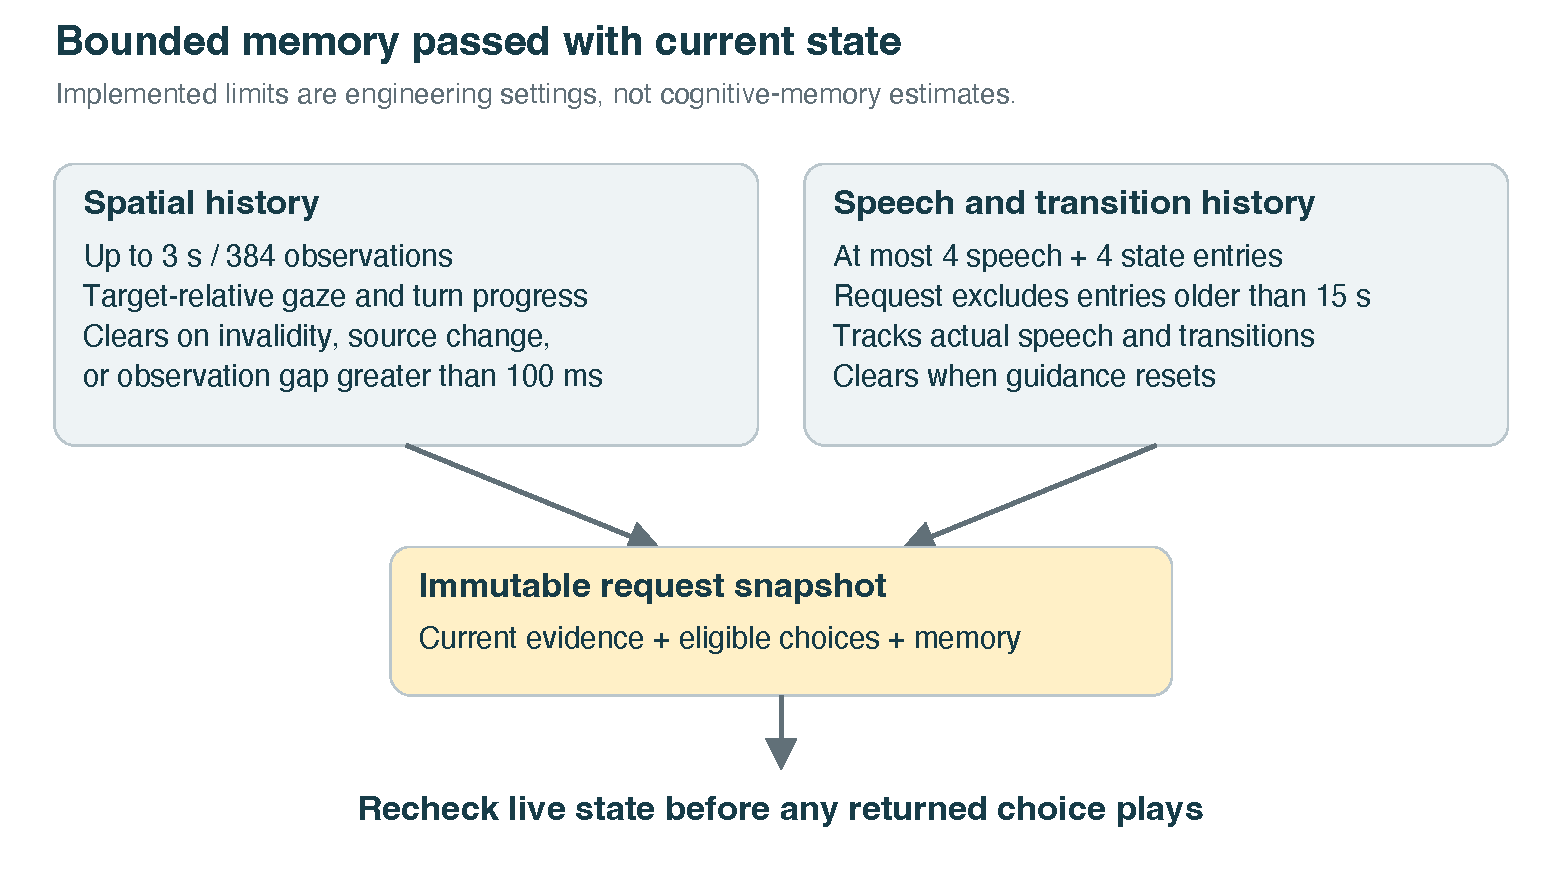
\includegraphics[width=\linewidth,alt={Spatial history and recent speech and state history are copied into a request and checked against current state before playback.}]{figures/bounded-memory.pdf}
\caption[Bounded spatial and speech memory]{Implemented memory limits and snapshot boundary. Spatial history and speech/state history have different retention and reset rules. A copied request preserves its original context, while playback still requires a fresh state check.}
\label{fig:bounded-memory}
\end{figure}


\section{Ownership and State Transitions}
The central guidance machine is a plain C\# object, while Unity MonoBehaviours connect it to tracked devices, scene objects, and audio; this arrangement separates deterministic state transitions from engine callbacks. Responsibility during a session is divided among three components. The round manager owns readiness, trial onset, completion, pause intervals, and block progression; the guidance machine owns the interpretation of evidence during search; and the speech scheduler owns pending requests, cancellation, and playback admission. The application is thus coordinated through distinct responsibilities rather than a single global state variable.

A state label is useful only when it is accompanied by its evidence. A refining state indicates that guidance has entered the target wall, but it does not prove that the eyes intersect the target object; likewise, an acquired state can reflect qualified vicinity evidence without implying that a trigger selection occurred. The viewer therefore presents state transitions alongside gaze-hit, vicinity-candidate, controller-hit, and playback records, so that an apparent disagreement can be inspected rather than the label being assumed to be complete ground truth.

\begin{table}[htbp]
\centering\caption{Guidance responsibilities and evidence boundaries.}
\small\tagpdfsetup{table/header-rows={1}}
\begin{tabularx}{\linewidth}{@{}p{0.22\linewidth}XX@{}}\toprule
Component & Owns & Does not establish \\\midrule
Observation adapters & Validity, poses, ray hits, source timing & Recognition or fixation \\
Guidance machine & Stage, eligible action, bounded history & Correct trigger selection or conscious recognition \\
Jev decision provider & Choice among eligible phrases; speak or wait & New target identity or unchecked geometry \\
Speech scheduler & Current-state check, pacing, cancellation, start & Acoustic arrival at the ear \\
Round manager & Readiness, reveal, selection, pauses and blocks & Independent validation of gaze accuracy \\
Trial Review & Reconstruction from saved evidence & Missing observations between recorded samples \\\bottomrule
\end{tabularx}
\end{table}

The usual path runs from turning toward a wall, through refinement within it and gaze acquisition of the target, to preparation for selection. This is not, however, a mandatory one-way chain: participants can overshoot, revisit a wall, point before gaze qualifies, or lose tracking. The implemented state families represent these returns, and release testing must verify them without the system repeatedly announcing a new arrival whenever the participant looks upward on the same wall. Invalid or stale evidence suspends new gaze-dependent decisions rather than being treated as a departure.

Figure~\ref{fig:guidance-states} summarizes the state families. The arrows show a common progression rather than compulsory transitions: correct right-trigger selection can complete an active trial without a preceding spoken gaze or pointing acknowledgment.

\begin{figure}[htbp]
\centering
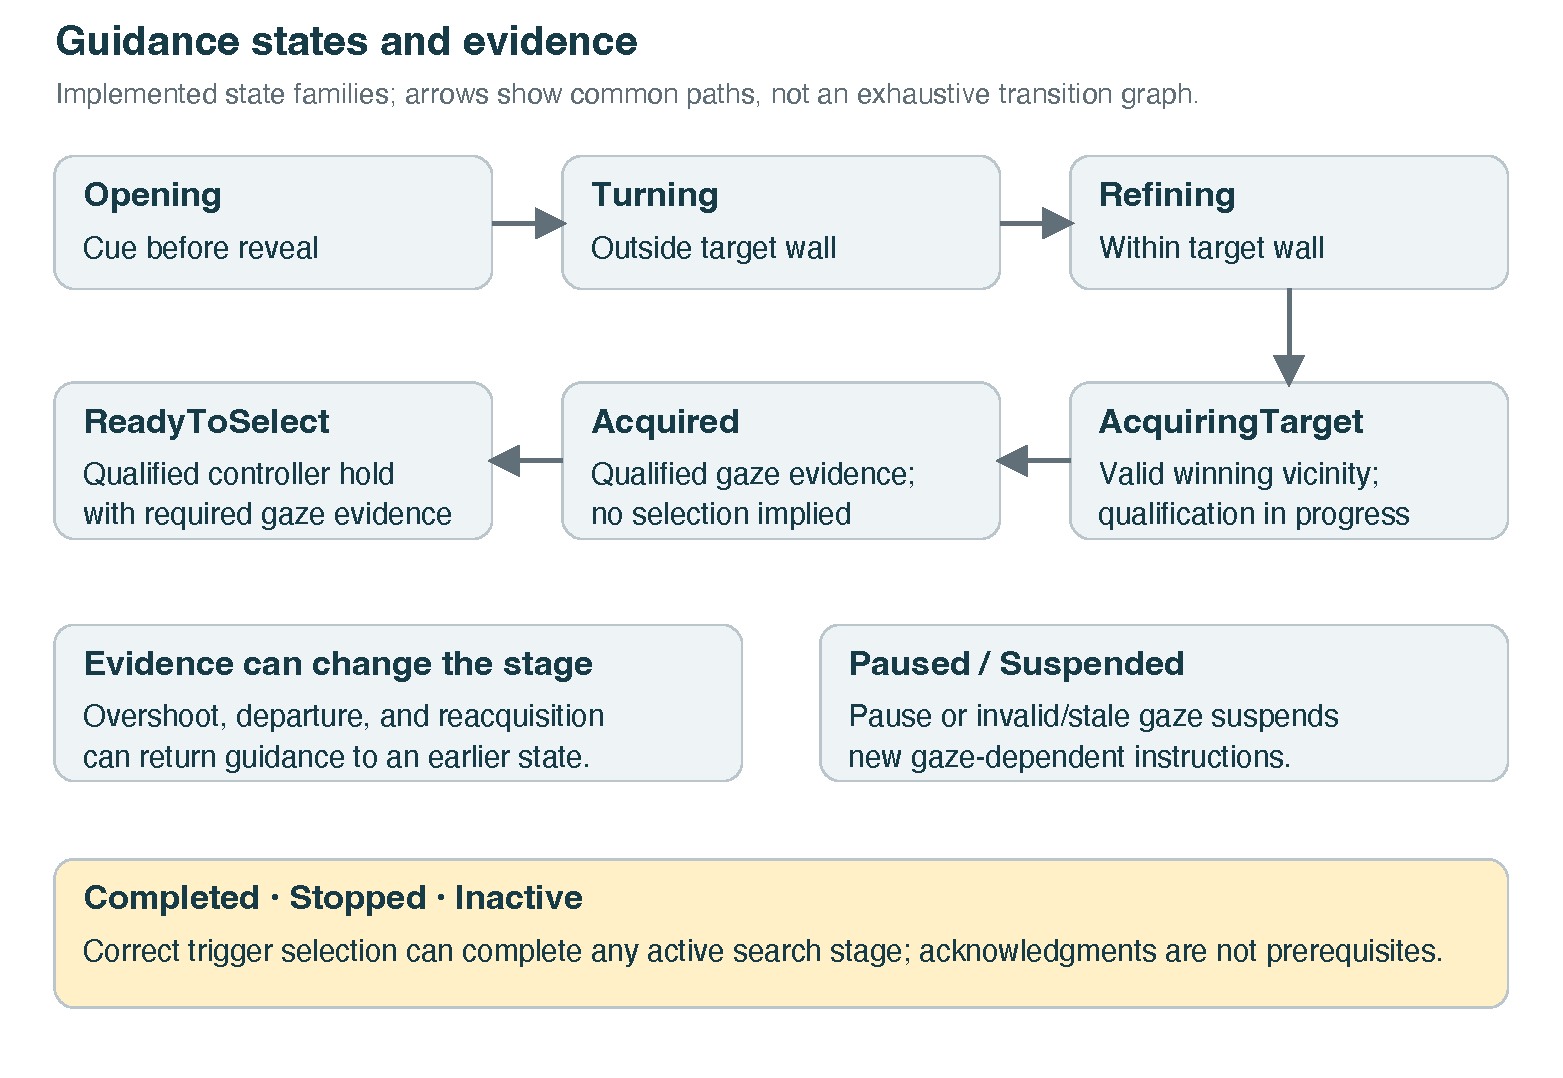
\includegraphics[width=\linewidth,alt={Common path from opening through turning and refinement to acquisition and readiness, with pause and suspension and independent trigger completion.}]{figures/guidance-states.pdf}
\caption[Guidance states and evidence-dependent transitions]{Implemented guidance state families. Turning, refining, acquisition, and readiness are evidence-dependent interpretations. Tracking loss, pauses, target departure, and reacquisition can change the path. Trial completion remains owned by the round manager.}
\label{fig:guidance-states}
\end{figure}


\section{A Worked Guidance Sequence}
Consider an illustrative target near the wall opposite the starting cross, with a rightward offset or the documented backward-turn tie rule. The opening cue may say that the object is to the right while objects remain hidden. Once search begins, progress cues can acknowledge continued rightward turning. On stable entry to the target wall, assistance can move to within-wall refinement, such as looking lower and slightly left. The reference for that refinement must be the recorded gaze geometry and local target relation, not a neighboring object's apparent screen position.

If the participant passes the target, recent spatial history can support a return cue. If the participant instead looks near the target long enough, a gaze acknowledgment becomes eligible, and if the controller is already intersecting the target, away-directions are suppressed immediately. A qualified pointing acknowledgment can then identify controller evidence, and a right-trigger press can complete the trial. This example illustrates intended transitions; it is not a measured trajectory or evidence that all people follow this sequence.

\section{Asynchronous Decisions and Cancellation}
Each cloud request receives a snapshot rather than a live reference to mutable state, comprising current evidence, relevant geometry, speech status, and bounded recent history. Because a response can become stale if the participant moves, tracking changes, the voice changes, a pause begins, or the trial ends, the scheduler checks these conditions again before playing the chosen clip. A valid answer to an old question is not necessarily a valid instruction now.

Prepared audio removes synthesis from the immediate hint path, but it does not remove network latency from cloud choice. Time-sensitive qualified feedback can therefore use local admission without waiting for another Jev decision, whereas ordinary hints can wait for a phrasing choice within bounded scheduling rules. Interruption policy balances urgency against comprehensibility, since finishing a short useful phrase may be preferable to cutting it at an awkward boundary. The documented implementation uses a 150-ms fade as a playback technique, not a guarantee of natural conversation.

Experimental policies that allow Jev broader action choice must be versioned separately from the participant policy. Replaying the same observations through multiple policies can compare decision latency and admissibility, but it cannot show how a participant would have moved after hearing a different cue. The participant release will therefore need one frozen policy and a manifest of thresholds, phrase library, Jev provider/model identifier, version, and available sampling settings. Whether the provider sees voice-condition identifiers must also be verified against the frozen payload. This draft does not assume condition-blind decisions, and that audit will distinguish voice-related cancellation keys from information actually transmitted to the provider.


\section{Operational Configuration and Reproducibility}
The method must preserve the conditions under which a decision was made, not only the selected phrase. A reproducibility record will bind the application revision to the gaze-source configuration, state-machine gates, phrase semantics, provider request contract, voice library, and instrument versions. Without that binding, a later replay can use the same target positions while silently changing the policy that produced the original speech.

Appendix~\ref{app:decision-contract} documents a code-inspected decision contract and a proposed release manifest. The inspection covers the recovered working implementation on October 23, 2026; it is not evidence that this working revision was merged, installed, or used by participants. In the inspected request builder, ordinary phrase selection uses a named choice question with eligible texts as keys in a criteria object, a combined request also asks whether to transmit, and returned selections must match the submitted candidates. The intended playback boundary additionally requires current-evidence rechecks, and the appendix distinguishes the inspected request and state code from release-wide checks still to be verified. Exact request and response records should accompany future claims about model behavior.

The application and external services have different reproducibility limits. Local geometry can be rerun from source and input fixtures, whereas a hosted model alias may resolve to a changed service even if its string is unchanged, and prepared audio can retain the original output while its provider's current synthesis changes. Accordingly, the study record will identify both configuration and realized outputs where permitted: actual candidate sets, returned choices, delivered clip identifiers, and playback events. A credential is never part of the research manifest.

No best-performing provider or autonomous policy is established by this manuscript. The offline comparison described below is a route to testing such alternatives. It must preserve the distinction between deciding what a model would say on a replayed trajectory and observing how a participant responds to that speech.

\section{Why Sequence Evaluation Is Necessary}
A phrase can be geometrically admissible in isolation and still be poor guidance in sequence. Repeating a direction immediately after it was delivered can be unnecessary, and a correct downward cue can become obsolete once the controller reaches the target. Likewise, a gaze acknowledgment can arrive late after multiple model waits even though each individual response was well formed. Evaluation must therefore inspect recent state, actions, and actual speech around the event.

Deterministic checks will first establish whether the evidence supports an action, distinguishing gaze confirmation, controller confirmation, and trial completion. A model judge may then use that evidence to assess the appropriateness of wording, timing, repetition, and interruption. Its ratings remain advisory: they do not represent human-perceived correctness, and they cannot convert an incompletely logged episode into a known success or failure.

\section{Paired Policy Pilots}
Paired pilots will feed identical recorded states and scripted trajectories to the baseline and candidate policies. The scenario set includes large turns, wall entry, vertical refinement, overshoot, gaze on target with the controller elsewhere, controller on target with nearby gaze, overlapping vicinity regions, blinks, stale tracking, pauses, and delayed model responses. Audio occupancy and readiness must also be represented so that playback admission can be compared fairly.

The candidate-policy comparison may include small, medium, and full eligible phrase sets. Full eligible means all choices that still satisfy hard geometry and validity requirements; it does not mean handing the model an unfiltered catalog and ignoring physical constraints. Provider support and exact candidate counts will be recorded. Experimental policies will remain outside participant builds until their results justify a controlled change.

Replaying an observed trajectory is a counterfactual engineering test. The original participant did not hear the alternative sequence, so the replay cannot demonstrate that the alternative would have reduced their search time. Scripted trajectories provide reproducible edge cases but are not measured human behavior. Both are useful for identifying faults before a wearer pilot.


\subsection{Development Cases and an Untouched Evaluation Set}
\textbf{Protocol proposal.} The engineering evaluation will maintain three explicitly labeled sources of cases: scripted fixtures that exercise known transitions and fault conditions, a development corpus of recorded sequences used to identify faults and tune policy, and a separate evaluation corpus held out from those tuning decisions. At this stage, no frozen split, sample count, or completed held-out score is claimed.

The split must occur at a level that prevents closely related observations from appearing on both sides. Adjacent requests from the same confirmation episode cannot be separated into development and evaluation as if they were independent cases. Where feasible, whole sessions, and participants when repeated sessions exist, will be assigned together. The release record will enumerate included sessions, duplicate checks, exclusions, and the moment at which the policy was frozen. It will identify each corpus as scripted, developer, pilot, or participant data. Participant-derived sequences will be replayed through hosted providers only where consent and data-handling terms permit. Previously inspected development runs cannot later be described as untouched evaluation data.

For a model-assisted judge, a human-reviewed calibration subset will define how the rubric is applied. Reviewers will see the same recorded evidence and mark unsupported conclusions as unknown. Disagreements will be retained, discussed, and used to clarify the rubric before evaluating the held-out set. A model judge's agreement with this subset is not a measure of participant perception. Repeatedly tuning the judge against the evaluation set would invalidate its held-out role just as repeated policy tuning would. The proposed review will mask policy labels and voice-condition identifiers where they are not required to interpret the evidence, while recording any residual clues that prevent effective blinding. Human--human and judge--human agreement statistics will be specified with the rubric before evaluation; unknown cases will retain their own reported count rather than silently disappear from denominators.

\subsection{Controlled Policy Comparisons}
Table~\ref{tab:policy-pilots} defines the comparison roles discussed during development. The table is a prospective evaluation design, not a report of measured winners. Candidate-set size and decision autonomy are separate manipulations: widening eligible wording while holding the action policy fixed does not test the same question as allowing the provider to choose a different action family.

\begin{table}[htbp]\centering
\caption[Proposed policy comparison and safeguards]{Engineering comparison roles. All policies retain valid input interpretation and explicit logging; experimental variants do not enter participant sessions on the basis of this table.}
\label{tab:policy-pilots}
\small\tagpdfsetup{table/header-rows={1}}
\begin{tabularx}{\linewidth}{@{}p{0.24\linewidth}XX@{}}\toprule
Policy role & Decision authority & What the comparison can test \\\midrule
Constrained Jev with local feedback & Local eligible action; provider chooses wording and speak/wait; qualified local feedback can bypass a new request. & Reference behavior and delivery delay under the shared scheduler. \\
Jev-led with local overrides & Provider considers meaningful eligible actions using state/history; local geometry, qualification, and final admission remain binding. & Whether broader choices improve sequence appropriateness without unacceptable delay. \\
Provider-led replay probe & Provider receives broad state and action choices; overrides are recorded as shadow checks rather than used to declare the model correct. & Unsupported choices and response timing offline. This is not an approved participant policy. \\\bottomrule
\end{tabularx}
\end{table}

The ordinary inspected request contract accepts two to five candidate phrases. A full-eligible-set experiment therefore requires an explicitly versioned test adapter when more than five candidates are eligible; this draft does not claim that the inspected request wrapper supports an arbitrary catalog size. Each pilot will log its actual candidate count, serialized payload size, request path, and model identifier. Small, medium, and full sets will be defined before execution rather than assigned favorable labels after observing results.

Paired execution will hold input timestamps, target geometry, validity, audio availability, and scoring rules constant. Model repetitions and execution order should be prespecified to expose stochastic variation and service-time effects. Independent request calls do not eliminate order-related network or server-load variation. Results will distinguish per-call transport measurements from whole-sequence behavior and will not substitute an average request latency for confirmation delivery time.

\section{Metrics and Episode Definitions}
For each policy, the report will summarize qualification-to-software-playback latency with median, 95th percentile, maximum, and count beyond a stated engineering threshold. The threshold must be declared before comparison and distinguished from a perceptual or clinical criterion. Episodes, rather than repeated requests within an episode, will be the denominator for delayed confirmations.

Jev request latency, failures, timeouts, calls per trial, cancellations, and late responses will be reported separately. A provider timeout can lead to a timely local fallback, while a successful provider response can still arrive too late for the current state. Provider reliability and delivered guidance reliability therefore require different measures.

Wrong-direction and stale hints will be labeled only when the available evidence shows that the instruction is unhelpful toward the task; a different but valid phrase is not automatically wrong, and missing evidence remains unknown. Judgments about repetition, unnecessary speech, excessive silence, and interruption appropriateness likewise require context beyond a sign check on an angle.

\section{Illustrative Failure Analysis}
An ordering failure can occur when a correction is queued before the controller reaches the target, and several distinct mechanisms could produce it. If playback checks use the older snapshot, the correction can play immediately before a pointing acknowledgment. Alternatively, the controller hold may not yet have qualified, leaving the ordinary-direction policy active during the hold, or action priority may admit a lower-priority cue despite newer pointing evidence. These causes require different fixes, yet they cannot be distinguished from the spoken text alone.

The intended correction is to suppress contradictory away-directions as soon as valid controller-on-target evidence is present, while retaining the independent qualification timer for the spoken pointing acknowledgment. A final playback check must repeat the suppression after any asynchronous wait or audio fade. If the controller leaves the target before qualification, no pointing acknowledgment should be emitted merely because the earlier request was valid.

A separate reference-frame problem arises when an object appears higher than a highlighted neighbor but the instruction says to look lower. If the instruction is calculated relative to the current eye ray, which could lie above both objects, the phrase can be geometrically consistent yet confusing because the highlight suggests a different reference object. Diagnosis therefore requires the recorded gaze ray, object positions, highlighted candidate, and playback time; it must not rely only on the review camera's screen-space layout.

These examples are diagnostic categories drawn from the development history. This appendix does not report their incidence or claim they have all been eliminated in a frozen participant build. The acceptance matrix in Appendix~\ref{app:scenarios} defines evidence required to make those claims.


\subsection{A Proposed Failure Taxonomy}
Table~\ref{tab:failure-taxonomy} classifies potential faults by where evidence is lost or acted on incorrectly. These categories organize review; they are not observed error rates. More than one category may contribute to an episode. When the trace does not establish a causal stage, the result remains unresolved rather than being assigned to Jev by default.

\begin{table}[htbp]\centering
\caption[Failure categories and diagnostic evidence]{Proposed sequence-review taxonomy. A label requires evidence from the relevant stage, and does not imply a frequency estimate.}
\label{tab:failure-taxonomy}
\small\tagpdfsetup{table/header-rows={1}}
\begin{tabularx}{\linewidth}{@{}p{0.24\linewidth}XX@{}}\toprule
Category & Diagnostic evidence & Example distinction \\\midrule
Observation or geometry & Validity, source age, coordinate frame, gaze ray, object transforms & Wrong spatial input versus a correct cue calculated from that input. \\
State or qualification & Gate timers, transition cause, controller hit, vicinity winner & Immediate pointing evidence versus qualified pointing acknowledgment. \\
Decision or context & Exact request snapshot, candidates, history, response & Unsupported choice versus an admissible alternative wording. \\
Scheduling or delivery & Cancellation, queue, final check, clip readiness, playback start/end & A valid old proposal that becomes stale before it speaks. \\
Interaction or reference & Visible highlight, task state, phrasing, recent speech & A geometric direction that is confusing relative to the highlighted neighbor. \\
Recording or scoring & Clock mapping, missing events, join version, episode identity & Missing evidence or duplicate counting versus a demonstrated runtime fault. \\\bottomrule
\end{tabularx}
\end{table}

\subsection{Worked Sequence Diagnosis}
The following cases are constructed examples, not participant observations. Their purpose is to show what evidence would justify a finding. Let $t_q$ be the first supported qualification and $t_p$ the actual software playback start, as defined in Chapter~\ref{ch:measurement}.

\begin{enumerate}
\item \textbf{A direction becomes stale during a controller hold.} A downward cue is eligible at request time. Before its response arrives, the tracked controller ray hits the target. The hold is not yet qualified, so a pointing acknowledgment would be premature. Under the intended policy, the search direction is suppressed and the hold gate preserved. If the old direction actually plays, the finding concerns admission or scheduling; if it was merely proposed and rejected, it is not a delivered wrong hint.
\item \textbf{Gaze qualifies while the controller remains elsewhere.} Valid winning-vicinity evidence satisfies the gaze gate at $t_q$. A looking acknowledgment is appropriate; a pointing acknowledgment is not. For a policy that routes this acknowledgment through the provider, repeated model waits followed by playback at $t_p$ form one delayed gaze-confirmation episode. Under the reference local-feedback path, a comparable delay would instead require investigation of scheduling, audio readiness, or delivery. Attribution requires the wait and scheduler records. It cannot be inferred from the final spoken text alone.
\item \textbf{The eyes and a nearby highlight imply different reference points.} The gaze ray is above both a target and a highlighted distractor, but the target is higher than that distractor. A lower cue may be consistent with the gaze ray while appearing wrong relative to the highlight. This warrants a reference-frame or wording concern, not an automatic wrong-sign label. The review must inspect the state at playback rather than only a screenshot after movement.
\end{enumerate}

For each reported real example, the completed thesis will provide the case-selection rule, a short surrounding timeline, the proposed versus played wording, the governing evidence, and the reason for the label. A few selected examples can explain a mechanism; they cannot establish its prevalence. Frequency claims require the defined evaluation denominator, including unknown and unreviewable episodes.

\section{Interpreting Two-Second Delays}
A two-second delay can contain several different intervals: waiting for qualification, waiting for a model response, an explicit model decision to wait, queued speech, audio readiness, and playback scheduling. Removing a provider wait does not establish that all delays disappear. Conversely, a one-second controller hold is an intentional qualification period, not necessarily a one-second processing fault.

The appropriate test starts from the first supported qualification for the particular event and ends at its actual software playback. A gaze event with a 100-ms gate and a controller event with a one-second hold must not share an undifferentiated origin. The report will retain both first evidence and qualification time so that readers can distinguish intentional gating from added delivery delay. Without a new verified sequence dataset and a wearer or acoustic measurement where required, this draft cannot claim that the roughly two-second delays have been removed.

\backmatter
\bibliographystyle{plain}
\bibliography{references}
\end{document}
